\documentclass[open=left,twopage=true]{scrreprt}

\usepackage{xspace}
\usepackage{amsmath}
\usepackage{amssymb}
\usepackage{latexsym}
\usepackage{pgf}
\usepackage{pgfarrows}
\usepackage{ntheorem}
\usepackage{lscape}
\usepackage{graphicx}
\usepackage{epic,eepic}
\usepackage{tikz}
\usetikzlibrary{automata,calc,shapes.geometric,arrows,shadings,chains}

% Kill any active \bfseries etc. with \normalfont to get the old behavior of \sc
\newcommand{\pgsolver}{{\normalfont\textsc{PGSolver}}\xspace}

\newcommand{\Nat}{\ensuremath{\mathbb{N}}}

\newcommand{\attr}[3]{\ensuremath{\mathit{Attr}^{#1}_{#2}(#3)}}

\newcounter{algcounter}
\newcounter{heurcounter}
\newcommand{\nextalg}{\stepcounter{algcounter}\arabic{algcounter}}
\newcommand{\nextheur}{\stepcounter{heurcounter}\arabic{heurcounter}}

\newcommand{\nonterminal}[1]{\ensuremath{\langle\mathit{#1}\rangle}}
\newcommand{\terminal}[1]{\ensuremath{\texttt{#1}}}
\newcommand{\sem}[1]{\ensuremath{[\![ #1 ]\!]}}
\newcommand{\hide}[1]{}

\newcommand{\TODOcomment}[2]{%
  \stepcounter{TODOcounter#1}%
  {\scriptsize\bf$^{(\arabic{TODOcounter#1})}$}%
  \marginpar[\fbox{
    \parbox{2cm}{\raggedleft
      \scriptsize$^{({\bf{\arabic{TODOcounter#1}{#1}}})}$%
      \scriptsize #2}}]%
  {\fbox{\parbox{2cm}{\raggedright
      \scriptsize$^{({\bf{\arabic{TODOcounter#1}{#1}}})}$%
      \scriptsize #2}}}
}%

\newcommand{\simpleTODOcomment}[2]{%
  \stepcounter{TODOcounter#1}%
  {\bf
    \scriptsize({\arabic{TODOcounter#1}~{#1}})
    {\bfseries{TODO:} #2}
  }
}

\newcounter{TODOcounter}
\newcommand{\TODO}[1]{\TODOcomment{}{#1}}
\newcommand{\TODOX}[1]{\simpleTODOcomment{}{#1}}


%%% Local Variables:
%%% mode: latex
%%% TeX-master: "main"
%%% End:

\definecolor{darkgreen}{rgb}{.1,.6,.1}
\definecolor{darkred}{rgb}{.6,.1,.1}

\definecolor{light-blue}{rgb}{0.7,0.8,1}
\usepackage[allbordercolors={light-blue},pdfborderstyle={/S/U/W 0.8}]{hyperref}

\begin{document}

\begin{titlepage}
\subject{Report}
\title{The \pgsolver Collection of Parity Game Solvers \\[2mm] {\large Version 4}}
\author{Oliver Friedmann \and Martin Lange \\[3mm]
Institut f\"ur Informatik \\ Ludwig-Maximilians-Universit\"at M\"unchen, Germany}
\publishers{
\vspace*{1cm}
\scalebox{0.8}{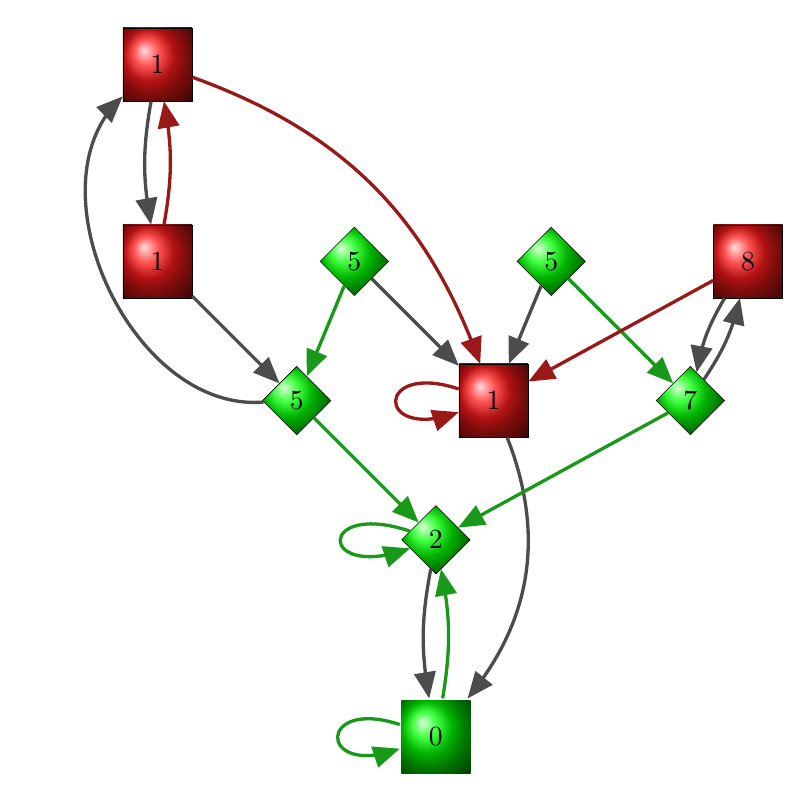
\begin{tikzpicture}[very thick,node distance=2.5cm,-triangle 45]
%\scalebox{0.59}{\includegraphics{graphics/titlegame}}

  \tikzstyle{redboxnode}=[draw=black,very thin,shape=rectangle,inner sep=10pt,ball color=red!90,shading=ball]
  \tikzstyle{reddiamnode}=[draw=red,shape=diamond]
  \tikzstyle{greenboxnode}=[shape=rectangle,inner sep=10pt,ball color=green,shading=ball]
  \tikzstyle{greendiamnode}=[draw=black,very thin,shape=diamond,ball color=green,shading=ball]

  \node[redboxnode]    (v0)                     {$1$};
  \node[redboxnode]    (v1) [below of=v0]       {$1$};
  \node[greendiamnode] (v2) [right of=v1]       {$5$};
  \node[greendiamnode] (v3) [right of=v2]       {$5$};
  \node[redboxnode]    (v4) [right of=v3]       {$8$};
  \node[greendiamnode] (v5) [below right of=v1] {$5$};
  \node[redboxnode]    (v6) [below right of=v2] {$1$};
  \node[greendiamnode] (v7) [below right of=v3] {$7$};
  \node[greendiamnode] (v8) [below right of=v5] {$2$};
  \node[greenboxnode]  (v9) [below of=v8]       {$0$};

  \path[black!70] (v0) edge [bend right=10] (v1)
                  (v1) edge                 (v5)
                  (v2) edge                 (v6)
                  (v3) edge                 (v6)
                  (v4) edge [bend right=10] (v7)
                  (v5) edge [bend left=70]     (v0)
                  (v6) edge [bend left]     (v9) 
                  (v7) edge [bend right=10] (v4)
                  (v8) edge [bend right=10] (v9);

  \draw[darkgreen] (v2) edge                 (v5)
                   (v3) edge                 (v7)
                   (v5) edge                 (v8)
                   (v7) edge                 (v8)
                   (v9) edge [bend right=10] (v8);

  \draw[darkred] (v0) edge [bend left=25]  (v6)
                 (v1) edge [bend right=10] (v0)
                 (v4) edge                 (v6);

  \draw[darkgreen] (v8) .. controls ($(v8)+(-1.5,.5)$) and ($(v8)+(-1.5,-.5)$) .. (v8);
  \draw[darkgreen] (v9) .. controls ($(v9)+(-1.5,.5)$) and ($(v9)+(-1.5,-.5)$) .. (v9);
  \draw[darkred]   (v6) .. controls ($(v6)+(-1.5,.5)$) and ($(v6)+(-1.5,-.5)$) .. (v6);

\end{tikzpicture}}}
\end{titlepage}
\maketitle[0]

\cleardoublepage
\pdfbookmark{Contents}{table-of-contents}
\tableofcontents

\chapter{Introduction}

\section{The Importance of Parity Games}

Parity games are simple two-player games of perfect information played on directed graphs whose
nodes are labeled with priorities. The name \emph{parity game} is due to the fact that the winner
of a play is determined according to the parities (even or odd) of the priorities occurring in
that play. In fact, it is determined by the maximal priority occurring infinitely often. % This
% can be seen as an abstraction of a setting in which an agent attemps to visit certain configurations
% infinitely often unless some other configurations are also visited infinitely often unless some
% other configurations are als visited infinitely often \ldots while another agent is making his/her
% life difficult by steering into different directions from time to time.

Parity games are an interesting object of study in computer science, and the theory of formal languages
and automata in particular, for (at least) the following reasons.
\begin{itemize}
\item They are closely related to other games of infinite duration like mean payoff games,
      discounted payoff games, stochastic games, etc.\ \cite{Jurdzinski/98,purithesis,Stirling95}.
\item They are at the core of other important problems in computer science, for instance, solving a
      parity game is known to be polynomial-time equivalent to model checking for the modal
      $\mu$-calculus \cite{Emerson93a,Stirling95}. 
\item They arise in complementation or determinisation problems for tree automata
      \cite{lncs2500,focs91*368} and in emptiness and word problems for various kinds of (alternating) 
      automata \cite{focs91*368}.
\item Controller synthesis problems can be reduced to satisfiability problems for branching-time logics
      \cite{AVW03} which in turn require the solving of parity games because
      of determinisations of B\"uchi word automata into parity automata 
      \cite{conf/lics/Piterman06,conf/icalp/KahlerW08}.
\item Solving a parity game is one of the rare problems that belongs to the complexity class
      NP$\cap$co-NP and that is not (yet) known to belong to P \cite{Emerson93a}. The variety of algorithms
      that have been invented for solving parity games is surely due to the fact that many people believe
      the problem to be in P.
\end{itemize}

\section{Aim and Content of \pgsolver}

This variety of algorithms has provided a good understanding of the theory of parity games even though
its computational complexity has possibly not yet been determined precisely. However, this theoretical
knowledge is unmatched by the little amount of investigation into practical aspects of solving parity
games. The aim of this project is to provide a platform for this: it should enable the comparison
between different algorithms not just by the Landau-terms for their worst-case time complexities but
by their actual performance on various classes of parity games.

The current version of this tool contains implementations of the following algorithms found in
the literature:
\begin{itemize}
\item the recursive algorithm due to Zielonka \cite{TCS::Zielonka1998},
\item the local model checking algorithm due to Stevens and Stirling \cite{StevensStirling98},
\item the strategy-improvement algorithm due to Jurdzi{\'n}ski and V\"oge \cite{conf/cav/VogeJ00},
\item the strategy-improvement algorithm due to Schewe \cite{conf/csl/Schewe08},
\item the strategy-improvement algorithm reduction to discounted payoff games due to Puri \cite{purithesis},
\item the randomized strategy-improvement algorithm due to Bj{\"o}rklund and Vorobyov \cite{BjoerklundVorobyov/2007},
\item another randomized strategy-improvement algorithm due to Bj{\"o}rklund, Sandberg and Vorobyov \cite{DBLP:conf/stacs/BjorklundSV03},
\item the small progress measures algorithm due to Jurdzi{\'n}ski \cite{Jurdzinski/00},
\item the small progress measures reduction to SAT due to Lange \cite{lange-gdv05},
\item the dominion decomposition algorithm due to Jurdzi{\'n}ski, Paterson and Zwick \cite{JPZ06},
\item the big-step variant of the latter due to Schewe \cite{Schewe/07/Parity}.
\end{itemize}
In addition, there is a new local strategy improvement algorithm by ourselves. Moreover
there is a direct reduction to SAT based on strategy iteration due to Friedmann.

Finally, there is one heuristic solvers. Such solvers are sound: the answers they provide are correct.
But they are not necessarily complete, for example because they may not terminate. Our heuristic
algorithm just guesses strategies for both players until a (partial) winning strategy has been found.

The heuristic is included because it can solve certain classes of parity games very quickly and
-- most importantly -- in a time that is independent of the number of priorities present in the game.
On the other hand, it is easy to construct games on which it does not terminate, resp.\ infinite families
of games on which the probability of termination decreases exponentially.



\section{Structure of this Report}

Chapter~\ref{chp:pgames} formally introduces parity games and standard notions around the problem of solving them
like winning regions and strategies, but also others that are needed in order to understand the constructions
implemented in various solvers like attractor strategies, decompositions into subgames, etc. It then
describes implemented meta-level optimisations for solving parity games, i.e.\ optimisations that apply to
\emph{any} solver. Next, it shortly describes the implemented algorithms and heuristics. For those known
before we refer to the corresponding literature for a detailed introduction into these algorithms. Here we
only want to point out the rough functionality in order to be able to compare these algorithms and possibly
attribute slow/fast solving to certain techniques.

Chapter~\ref{chp:uguide} is the user's guide. It describes how to compile, install and run \pgsolver, as well
as how to specify parity games that it takes as input and how to read its output, etc.

\pgsolver comes with programs that generate benchmarks. These are for example random games, games
constructed in a way such that they are difficult for a certain algorithm to solve, or application-oriented
games. These are described in Chapter~\ref{chp:benchmarks}.

Finally, Chapter~\ref{chp:devguide} contains the developer's guide. It explains how to
integrate another parity game solver -- implemented in OCaml -- into this tool.

%%% Local Variables:
%%% mode: latex
%%% TeX-master: "main"
%%% End:


\chapter{Solving Parity Games}
\label{chp:pgames}

\section{Technicalities}

\subsection{Parity Games}

A \emph{parity game} is a tuple $G = (V,V_0,V_1,E,\Omega)$ where $(V,E)$ forms a directed graph
whose node set is partitioned into $V = V_0 \cup V_1$ with $V_0 \cap V_1 = \emptyset$, and
$\Omega : V \to \Nat$ is the \emph{priority function} that assigns to each node a natural number
called the \emph{priority} of the node. We assume the underlying graph to be total, i.e.\ for every
$v \in V$ there is a $w \in W$ s.t.\ $(v,w) \in E$.

We also use infix notation $vEw$ instead of $(v,w) \in E$ and define the set of all \emph{successors} of
$v$ as $vE := \{ w \mid vEw \}$, as well as the set of all \emph{predecessors} of $w$ as
$Ew := \{ v \mid vEw \}$.

The game is played between two players called $0$ and $1$ in the following way. Starting in a node
$v_0 \in V$ they construct an infinite path through the graph as follows. If the construction so far
has yielded a finite sequence $v_0\ldots v_n$ and $v_n \in V_i$ then player $i$ selects a $w \in v_nE$
and the play continues with the sequence $v_0\ldots v_n w$.

Every play has a unique winner given by the \emph{parity} of the greatest priority that occurs infinitely 
often in a play. The winner of the play $v_0 v_1 v_2 \ldots$ is player $i$ iff
$\max \{ p \mid \forall j \in \Nat \exists k \geq j:\, \Omega(v_k) = p \} \equiv_2 i$ (where $i \equiv_2 j$ holds iff $|i - j| \mod 2 = 0$). That is, player $0$ tries to make an even
priority occur infinitely often without any greater odd priorities occurring infinitely often, player
$1$ attempts the converse.

% The priorities occurring in a game are often ordered w.r.t. their usefulness to one of the players $i \in \{0, 1\}$ by the \emph{reward order $\preceq_i$} which is defined as follows:
% \begin{displaymath}
% p_1 \preceq_i p_2 \,:\iff\,\, rew_i(p_1) \leq rew_i(p_2)
% \end{displaymath}
% where $rew_i(p) := p$ if $p \equiv_2 i$ and $rew_i(p) := -p$ otherwise.
% \TODO{Paragraph nach hinten}

In the following we will restrict ourselves to finite parity games. It is easy to see that in a finite
parity game the winner of a play is determined uniquely since the range of $\Omega$ must necessarily
be finite as well. Technically, we are considering so-called max-parity games. There is also the
min-parity variant in which the winner is determined by the parity of the \emph{least} priority occuring
infinitely often. On finite graphs, though, these two games are equivalent in the sense that a max-parity
game $G = (V,V_0,V_1,E,\Omega)$ can be converted into a min-parity game $G' = (V,V_0,V_1,E,\Omega')$
whilst preserving important notions like winning regions, strategies, etc. Simply let $p$ an even upper
bound on all the priorities $\Omega(v)$ for any $v \in V$. Then define $\Omega'(v) := p - \Omega(v)$.
This construction also works the other way round, i.e.\ in order to transform a min-parity into a
max-parity game.

A \emph{strategy} for player $i$ is a partial function $\sigma: V^*V_i \to V$, s.t.\ for all sequences
$v_0 \ldots v_n$ with $v_{i+1} \in v_iE$ for all $j=0,\ldots,n-1$, and all $v \in V_i$:
$\sigma(v_0\ldots v_n) \in v_nE$. That is, a strategy for player $i$ assigns to every finite path through
$G$ that ends in $V_i$ a successor of the ending node. A play $v_0 v_1 \ldots$ \emph{conforms} to a strategy
$\sigma$ for player $i$ if for all $j \in \Nat$ we have: if $v_j \in V_i$ then 
$v_{j+1} = \sigma(v_0\ldots v_j)$.
Intuitively, conforming to a strategy means to always make those choices that are prescribed by the strategy.
A strategy $\sigma$ for player $i$ is a \emph{winning strategy} starting in some node $v \in V$ if player $i$ wins
every play that conforms to this strategy and begins in $v$. We say that player $i$ \emph{wins} the game $G$
starting in $v$ iff he/she has a winning strategy for $G$ starting in $v$.

With $G$ we associate two sets $W_0,W_1 \subseteq V$ with the following definition. $W_i$ is the set of
all nodes $v$ s.t.\ player $i$ wins the game $G$ starting in $v$. We write $W_i^G$ in order to name the parity 
game that the winning regions refer to, for example when it cannot uniquely be identified from the context. 

Clearly, we must have
$W_0 \cap W_1 = \emptyset$ for otherwise assume that there is a node $v$ such that both players $0$ and $1$
have winning strategies $\sigma_0$ and $\sigma_1$ for $G$ starting in $v$. Then there is a unique play
$\pi = v_0 v_1 \ldots$ such that $v_0 = v$ and $\pi$ conforms to both $\sigma_0$ and $\sigma_1$. It is
obtained by simply playing the game while both players perform their choices according to their respective
strategies. However, by definition $\pi$ is won by both players, and therefore the maximal priority occurring
infinitely often would have to be both even and odd.

On the other hand, it is not obvious that every node should belong to either of $W_0$ or $W_1$. However, this
is indeed the case and known as \emph{determinacy}: a player has a strategy for a game iff the opponent does
not have a strategy for that game.

\begin{theorem}[\cite{Mart75,Gurevich-Harrington/82,focs91*368}]
Let $G = (V,V_0,V_1,E,\Omega)$ be a parity game. Then $W_0 \cap W_1 = \emptyset$ and $W_0 \cup W_1 = V$.
\end{theorem}

A strategy $\sigma$ for player $i$ is called \emph{positional} or \emph{memory-less} or \emph{history-free} if
for all $v_0\ldots v_n \in V^*V_i$ and all $w_0\ldots w_m \in V^*V_i$ we have: if $v_n = w_m$ then
$\sigma(v_0\ldots v_n) = \sigma(w_0\ldots w_m)$. That is, the value of the strategy on a finite path
only depends on the last node on that path. An important feature of parity games is the fact that such
strategies suffice.

\begin{theorem}[\cite{focs91*368}]
Let $G = (V,V_0,V_1,E,\Omega)$ be a parity game, $v \in V$, and $i \in \{0,1\}$. Player $i$ has a winning
strategy for $G$ starting in $v$ iff player $i$ has a positional winning strategy for $G$ starting in $v$.
\end{theorem}

A positional strategy $\sigma$ for player $i$ induces a \emph{subgame} 
$G|_\sigma := (V, V_0, V_1, E|_\sigma, \Omega)$ where 
$E|_\sigma := \{(u, v) \in E \mid u \in dom(\sigma) \Rightarrow \sigma(u) = v\}$. Such a subgame $G|_\sigma$ 
is, roughly speaking, basically the same game as $G$ with the restriction that whenever $\sigma$ provides a 
strategy decision for a node $u \in V_i$ all transitions from $u$ but $\sigma(u)$ are no longer accessible.

A set $U \subseteq V$ is said to be $i$-closed iff player $i$ can force any play to stay within $U$. This
means that player $1-i$ must not able to leave $U$ but player $i$ must always have the choice to remain 
inside $U$: 
\begin{displaymath}
\forall v \in U:\, \big(\ v \in V_{1-i}\, \Rightarrow \, vE \subseteq U\ \big)
\enspace \mbox{and} \enspace
\big(\ v \in V_i\, \Rightarrow \, vE \cap U \ne \emptyset\ \big)
\end{displaymath}
Note that $W_0$ is $0$-closed and $W_1$ is $1$-closed.

A set $U \subseteq V$ induces a \emph{subgame} 
$G|_U := (U, U \cap V_0, U \cap V_1, E \cap U \times U, \Omega|_U)$ iff the underlying transition relation 
$E \cap U \times U$ remains total i.e. for all $u \in U$ there is at least one $v \in U$ s.t.\ $uEv$. Clearly, 
each $i$-closed set $U$ induces a subgame. We often identify a set $U \subseteq V$ that induces a subgame 
w.r.t.\ a fixed parity game with the induced subgame itself.

\subsection{Dominions}

A set $U \subseteq V$ is called an \emph{$i$-dominion} iff $U$ is $i$-closed and the induced subgame is won by player $i$. Clearly, $W_0$ is a $0$-dominion and $W_1$ is a $1$-dominion. That is, an $i$-dominion $U$ covers the idea of a region in the game graph that is won by player $i$ by forcing player $1-i$ to stay in $U$ on the one hand; but on the other hand an $i$-dominion $U$ is only won by player $i$ when using a winning strategy on $U$.

To see more precisely what the concept of dominions is used for we need to introduce \emph{attractors} and 
\emph{SCC decompositions} of parity games.


\subsection{Attractors and Attractor Strategies}
Let $U \subseteq V$ and $i \in \{0,1\}$. Define for all $k \in \Nat$
\begin{align*}
\attr{0}{i}{U} \enspace := \enspace &U \\
\attr{k+1}{i}{U} \enspace := \enspace &\attr{k}{i}{U} \\
\cup\enspace &(V_i \cap \{ v \mid vE \cap \attr{k}{i}{U} \ne \emptyset \}) \\
\cup\enspace &(V_{1-i} \cap \{ v \mid vE \subseteq \attr{k}{i}{U} \}) \\
\attr{}{i}{U} \enspace := \enspace &\bigcup\limits_{k \in \Nat} \attr{k}{i}{U}
\end{align*}
Intuitively, $\attr{k}{i}{U}$ consists of all nodes s.t.\ player $i$ can force any play to reach $U$ in
at most $k$ moves. 
%Attractors are necessary in order to be able to use local solvers for the global problem.

\begin{lemma}[\cite{TCS::Zielonka1998,Stirling95}]
\label{lem:minusattr}
Let $G = (V,V_0,V_1,E,\Omega)$ be a parity game and $U \subseteq V$. Let $V' := V \setminus \attr{}{i}{U}$.
Then $G' = (V',V_0 \cap V',V_1 \cap V', E \cap V'\times V',\Omega)$ is again a parity game with its
underlying graph being total.
\end{lemma}

In other words $V \setminus \attr{}{i}{U}$ is $(1-i)$-closed; if additionally $U$ is an $i$-dominion then 
$\attr{}{i}{U}$ also is an $i$-dominion. This yields a general procedure for solving parity games: find a 
dominion in the game graph that is won by one of the two players, build its attractor of the dominion and 
investigate the complement subgame.

Each attractor for player $i$ induces an \emph{attractor strategy} for player $i$. It is defined for all
$v \in \attr{k}{i}{U} \cap V_i$ for any $k \ge 1$ as $\sigma(v) = w$ iff $w \in \attr{k-1}{i}{U}$.









%%% Local Variables:
%%% mode: latex
%%% TeX-master: "main"
%%% End:

\section{Local vs.\ Global Solvers}

The problem of \emph{solving} a parity game $G = (V,V_0,V_1,E,\Omega)$ is, roughly speaking, to determine
which of the players has a winning strategy for that game. However, this does not take starting nodes into
account. In order to obtain a well-defined problem, this is refined in two ways.

The problem of solving the parity game $G$ \emph{globally} is to determine, for \emph{every} node $v \in V$
whether $v \in W_0$ or $v \in W_1$. The problem of solving $G$ \emph{locally} is to determine for a
\emph{given} $v \in V$ whether $v \in W_0$ or $v \in W_1$ holds. In addition, we require a \emph{solver}
to compute (partial) winning strategies in the following sense: a local solver should return one strategy
that is a winning strategy for player $i$ if $v \in W_i$ for the given input node $v$. A global solver
should return two strategies, one for each player s.t.\ player $i$ wins exactly on the nodes $v \in W_i$
if he/she plays according to the strategy computed for her.

Clearly, the local and global problem are interreducible, the global one solves the local one for free,
and the global one is solved by calling the local one $|V|$ many times. But neither of these indirect
methods is particularly clever. Thus, there are algorithms for the global, and other algorithms for the
local problem. We focus on the global problem here, but also use local solvers. In that case we expect
them to determine for \emph{at least} the given node $v$ to which winning set it belongs but possibly and
preferably also for other nodes. These methods can then be used to solve the global problem by calling
the local algorithm \emph{at most} $|V|$ many times.

Suppose $V = \{v_0,\ldots,v_n\}$. Then one can solve $G$ globally using a local solver $A$ as follows.
Start $A$ with starting node $v_0$. It will return two (possibly empty) winning sets $W'_0$ and $W'_1$.
In any case, we will have $W'_0 \cap W'_1 = \emptyset$, but not necessarily $W'_0 \cup W'_1 = V$. Let
$W' := V \setminus (\attr{}{0}{W'_0} \cup \attr{}{1}{W'_1})$. Then taking out all nodes in $W'$ from $G$
will result in a total parity game again by two applications of Lemma~\ref{lem:minusattr} and the fact
that $\attr{}{0}{W'_0} \cap \attr{}{1}{W'_1} = \emptyset$. Let $G'$ be this game. Then the winning positions
for player $i$ in $G$ are $\attr{}{i}{W'_i}$ plus the winning positions for him/her in $G'$. Since $G'$
will be smaller than $G$ this can be used iteratively or recursively, to compute the entire $W_0$ and $W_1$.

The winning strategies can equally be assembled to a winning strategy $\sigma$ for player $i$. Let
$\sigma'$ be player $i$'s winning strategy on the subgame $G'$, $\alpha$ be his/her attractor strategy
for reaching $W'_i$, and $\eta$ be the strategy that guarantees him/her to win on $W'_i$. Then define
\begin{displaymath}
\sigma(v) \enspace := \enspace
\begin{cases}
\eta(v) \enspace, &\mbox{if } v \in W'_i \\
\alpha(v) \enspace, &\mbox{if } v \in \attr{}{i}{W'_i} \setminus W'_i \\
\sigma'(v) \enspace, &\mbox{if } v \mbox{ is a node in } G' \\
\mbox{anything} & \mbox{otherwise}
\end{cases}
\end{displaymath}
The following theorem provides correctness of this construction. 

\begin{proposition}
Let $G = (V,V_0,V_1,E,\Omega)$ be a parity game, let $W_i$ be the winning set of player $i$ and 
$i \in \{0,1\}$. Player $i$ has a positional strategy $\sigma$ for $G$ s.t. $\sigma$ is a positional 
winning strategy for $G$ starting in any node $v \in W_i$.
\end{proposition}

To see that this holds let $\sigma_v$ be positional winning strategies for $G$ starting in $v$ for each node 
$v \in W_i$ (which have to exist by the former theorem). We assume all nodes $v \in W_i$ to be ordered 
w.r.t.\ a well-ordering $<$. A positional strategy $\sigma$ winning from each node $v \in W_i$ can be 
defined as follows:
\begin{displaymath}
\sigma: v \in W_i \cap V_i \mapsto \sigma_{\min_{<} \{u \in W_i \mid v \in dom(\sigma_u)\}} (v)
\end{displaymath}
To see that $\sigma$ indeed is a positional winning strategy for $G$ starting in any node $v \in W_i$ let 
$v_0 v_1 \ldots$ be a $\sigma$-conforming play with $v_j \in W_i$ for all $j \in \Nat$. Since $<$ is a 
well-ordering $\sigma$ finally simulates the strategy of $\sigma_u$ for some $u \in W_i$ and thus player 
$i$ is wins this play.





%%% Local Variables:
%%% mode: latex
%%% TeX-master: "main"
%%% End:

\section{Verifying Strategies}

The problem of \emph{verifying strategies} is to decide whether a given partition $(W'_0, W'_1)$ of a parity 
game $G$ along with two strategies $\sigma_0: W'_0 \cap V_0 \rightarrow V$ and 
$\sigma_1: W'_1 \cap V_1 \rightarrow V$ matches the partition into winning sets, i.e. whether $W'_0 = W_0$ 
and $W'_1 = W_1$ as well as $\sigma_0$ and $\sigma_1$ ensure the win of the respective player in the 
respective winning set.

The verification process basically traverses three phases. The algorithm verifies in the first phase that 
$\sigma_0$ and $\sigma_1$ are welldefined in the sense that a strategy actually uses valid transitions in 
the game graph. In the second phase the algorithm checks whether the strategies stay in their winning 
regions, i.e. $\sigma_i[W'_i] \subseteq W'_i$ for both player $i$, as well as whether the winning regions 
are closed w.r.t. the respective player.

The third phase finally checks whether the given strategies are winning strategies. In order to solve this 
problem, the algorithm computes the subgames $G_i := (G|_{W'_i})|_{\sigma_i}$ induced by the respective sets 
and strategies in question. Note that both $G_i$ are special games, namely one-player games. Hence, they
can be solved as described above.

Since $\sigma_i$ is a winning strategy on $W'_i$ iff $\sigma_i$ is a winning strategy on $G_i$, it suffices 
to check whether the computed winning set $W^{G_i}_i$ correspond with 
$W'_i$, and if they do not, the counter strategy for player $1 - i$ can be used to extract a cycle in $G$ 
following strategy $\sigma_i$ that is won by $1-i$.




%%% Local Variables:
%%% mode: latex
%%% TeX-master: "main"
%%% End:

\section{Universal Optimisations}
\label{sec:universal}

There are some optimisations that apply to \emph{all} solvers. These universal optimisations efficiently
try to reduce the overall complexity of a given parity game in order to reduce the effort spent by any solver. 
Clearly, such optimisations have to ensure that a solution of the modified game can be effectively and 
efficiently translated back into a valid solution of the original game.

In the following we describe optimisations that are implemented on top of every solving algrithm:
SCC decomposition, detection of special cases, and compression. The next section then describes a generic
algorithm that uses (some of -- depending on the configuration) these optimisations in order to call
a real solver on as few and little parts of a game as possible.   


\subsection{SCC Decomposition}

Let $G = (V, V_0, V_1, E, \Omega)$ be a parity game. A \emph{strongly connected component} (SCC) is a non-empty set 
$S \subseteq V$ with the property that every node in $S$ can reach every other node in $S$, i.e. $uE^*v$ for 
all $u, v \in S$ (where $E^*$ denotes the transitive-reflexive closure of $E$). A strongly connected component 
$S$ is \emph{proper} iff $uE^+v$ for all $u, v \in S$ (where $E^+$ denotes the transitive closure of $E$). In 
other words: An SCC $S$ is proper iff $|S| > 1$ or $S = \{u\}$ and $uEu$.

\begin{theorem}[\cite{tarjan:146}]
Every parity game $G = (V,V_0,V_1,E,\Omega)$ can, in time $\mathcal{O}(|E|)$, be partitioned into SCCs 
$S_0, ..., S_n$ with $V = \bigcup_{i \leq n} S_i$ and $S_i \cap S_j = \emptyset$ for all $i \not= j$.
\end{theorem}

Additionally there is a strict partial ordering $\rightarrow$ on these SCCs which is defined as follows:
\begin{displaymath}
S_i \rightarrow S_j \quad:\iff\quad i \not= j \wedge \exists u \in S_i,\, v \in S_j:\, uEv
\end{displaymath}
This strict partial ordering is generally known as the \emph{topology} of the SCC decomposition. An SCC $S$
is called \emph{final} w.r.t.\ $\to$ if there is no SCC $T$ s.t.\ $S \to T$. Note that every SCC topology
of a finite graph must have at least one final SCC.

SCC decomposition of parity games as a universal optimisation works as follows. First, the game is decomposed 
into SCCs along with the computation of the strict partial ordering $\rightarrow$. Then, all final SCCs 
with respect to $\rightarrow$ are solved by a parity game solver. Since these SCCs are not connected to any 
other SCCs, all solutions obtained in this manner can be directly used as solutions in the global game.

Second, the attractors for both players with respect to the computed winning sets of all maximal solved SCCs 
are computed and removed from the game. The remainder is still a game, but because of the removal some of the
original SCCs may not be SCCs anymore. All ``damaged'' ex-SCCs are again decomposed into SCCs and replaced by 
the new respective decomposition. 
%(Note: There is no need to actually replace the SCC in the data structure; it is more convenient to implement
% this by recursion).
In this way, the remaining decomposition can be used again to solve the rest of the game, again starting
with those SCCs that are now final. 
%Note that it is convenient to automatically solve improper SCCs since otherwise they usually need to be 
%treated differently than normal SCCs in the real solving algorithms.


%\subsection{Excision of Dominions}

%Although there is no obvious way to further reduce a parity game to smaller sub games that need to be solved, 

With this SCC decomposition it is not necessary to require solvers to solve an entire SCC let alone an entire
game. Instead it suffices to have them solve at least a dominion for one of the players. Given an SCC $S$ and
two dominions $D_0, D_1 \subseteq S$ with $D_0 \subseteq W_0$ and $D_1 \subseteq W_1$, one simply computes the 
attractors $A_i := \attr{}{i}{D_i}$ and considers the induced subgame $(S \setminus A_0) \setminus A_1$ which 
can be recursively solved by decomposition into SCCs etc.

% The excision of dominions is particularly useful for algorithms using a certain heuristic to generate ``good'' 
% strategies or for algorithms trying to find small dominions locally; some solution algorithms of the following 
% subsection will apply the dominion excision approach. Since the excision of a dominion possibly leads to a new 
% subgame that can be optimised and decomposed again, this optimisation can be very powerful.\TODO{Sehr schwammiger
% Paragraph.}


\subsection{Detection of Special Cases}

There are certain kinds of special games that can be solved very efficiently by the following procedures. 
W.l.o.g.\ we can assume games to be proper strongly connected components. Remember that SCCs which are not proper
consist of a single node $v$ only that does not have an edge back to itself. The winner of $v$ is the owner
iff there is a successor that he/she wins. Since all successors belong to topologically greater SCCs we can
assume them to be solved already, and thus, the winner of $v$ is easily determined.

\begin{itemize}
\item \emph{Self-cycle games}: Suppose there is a node $v$ such that $vEv$. Then there are two cases depending on
the node's owner $p$ and the parity of the node's priority. If $\Omega(v) \not\equiv_2 p$ then taking the edge 
$(v,v)$ is always a bad choice for player $p$ and this edge can be removed from the game for as long as 
totality is preserved. If $\Omega(v) \equiv_2 p$ then taking this edge is always good in the sense that 
$\{v\}$ is a dominion for player $p$. Hence, its attractor can be removed as described above.

\item \emph{One-parity games}: If all nodes in a proper SCC have the same parity, the whole game is obviously won 
by the corresponding player no matter which transition the player uses. Hence, a winning strategy can be found 
by random choice.

\item \emph{One-player games}: A game $G$ is a one-player game for player $i$ iff for all $v \in V_{1 - i}$ we have
$|vE| = 1$. Such a one-player game that is an SCC can be solved using a simple fixed-point iteration. 
%\begin{align*}
%E_0\,\, &:= E \\
%E_{j + 1} &:= \{(u, v) \mid uE_jv \vee \exists w:(uE_jw \wedge wE_jv \wedge \Omega(u) \geq \Omega(w) \wedge \Omega(u) \equiv_2 i )\} \\
%E'\,\, &:= \bigcup_{j \in \Nat} E_j
%\end{align*}
%Now the following holds: 
Player $i$ wins the game iff there is a node $u$ with $\Omega(u) \equiv_2 i$ and $u$ is reachable from itself
on a path that does not contain a priority greater than $\Omega(u)$.
% As player $i$ wins the game iff there is a cycle in the game won by player $i$ the fixed point iteration 
%simply computes which nodes having parity $i$ can reach itself without seeing a greater priority than their 
%own. Thus, if $E'$ connects $i$-parity nodes with itself, there needs to be a cycle using that particular 
%node being won by player $i$. The conversion also holds: If there is no $i$-parity node $u$ s.t. $uE'u$ then 
%the whole SCC is won by player $1-i$.
If there is such a cycle won by player $i$ then the rest of the SCC lies in the attractor of the cycle (since 
player $i$ is the only one to make choices); otherwise, if there is no cycle won by player $i$, the whole game 
is won by player $1-i$.
\end{itemize}


\subsection{Priority Compression}

The complexity of a parity game rises with the number of different priorities in the game. This optimisation step
attempts to reduce this number. Note that it is not the actual values of priorities that determine the winner.
It is rather their \emph{parity} on the one hand and their \emph{ordering} on the other. For instance, if there are 
two priorities $p_1 < p_2$ in a game with $p_1 \equiv_2 p_2$ but there is no $p'$ such that $p_1 < p' < p_2$ and 
$p' \not\equiv_2 p_1$ then every occurrence of $p_2$ can be replaced by $p_1$. 

In general, let $P = (p_0,\ldots,p_k)$ be the list of all the priorities occurring in a game $G = (V,V_0,V_1,E,\Omega)$ 
s.t.\ $p_{i-1} < p_i$ for all $0 \le i < k$. W.l.o.g.\ we assume $p_0$ to be even. If the least priority occurring in
$G$ is odd, then simply add $p_0 = 0$ to this list which does not affect the construction in any way. We will also
use $P$ to denote the \emph{set} of all elements in $P$.

Take a decomposition of $P$ into maximal sublists of elements with the same parity, i.e.\ 
\begin{displaymath}
P \enspace = \enspace (p_{0,0},\ldots,p_{0,m_0},p_{1,0},\ldots,p_{1,m_1},\ldots,p_{n,0},\ldots,p_{n,m_n})
\end{displaymath}
with $p_{i,j} \equiv_2 p_{i,j'}$ for all $0 \le i \le n$, $0 \le j < j' \le m_i$ and 
$p_{i,m_i} \not\equiv_2 p_{i+1,0}$ for all $0 \le i < n$. This defines a partial mapping $\omega: \Nat \to \Nat$ as 
\begin{displaymath}
\omega(p) \enspace = \enspace 
\begin{cases} 
i &, \mbox{if } p = p_{i,j} \mbox{ for some } j  \\
\mathrm{undefined} &, \mbox{otherwise}
\end{cases}
\end{displaymath}
Note the following facts about $\omega$:
\begin{itemize}
\item $\omega$ is defined on all priorities occurring in $G$;
\item $\omega$ is \emph{decreasing}: we have $\omega(p) \le p$ for all $p \in P$;
\item $\omega$ is \emph{monotone}: for all $p,p'$ with $p \le p'$ we have $\omega(p) \le \omega(p')$;
\item $\omega$ \emph{preserves parities}: we have $\omega(p) \equiv_2 p$ for all $p \in P$;
\item $\omega$ is \emph{dense}: for all $p,p' \in P$ with $\omega(p)+1 < \omega(p')$ there is a $p''$ with 
$\omega(p) < \omega(p'') < \omega(p')$.
\end{itemize} 
Now define another parity game $G' := (V,V_0,V_1,E,\Omega')$ with $\Omega'(v) := \omega(\Omega(v))$. I.e.\ $G'$
results from $G$ by reducing the priorities according to the function $\omega$. Then $G'$ is equivalent to $G$
in the sense that the players' winning regions coincide in the two games, and a winning strategy $\sigma$ for
some player $i$ in $G$ is also a winning strategy for him/her in $G'$ and vice-versa. This is guaranteed by the
properties of $\omega$ identified above: due to monotonicity and preservation of parities, the greatest priority
ocurring in an infinite play in $G$ is even iff it is even in the same play in $G'$. The property of being
decreasing guarantees that this should in general be an optimisation, and density says that $G'$ is optimal 
w.r.t.\ this optimisation. 
 
% \begin{lemma}
% Every parity game $G = (V,V_0,V_1,E,\Omega)$ induces an equivalent parity game $G' = (V,V_0,V_1,E,\Omega')$ where 
% $\Omega'$ is inductively defined as follows:
% \begin{displaymath}
% \Omega'(v) \enspace := \enspace
% \begin{cases}
% m(v) \enspace, &\mbox{if } \Omega(v) \equiv_2 m(v) \\
% m(v) + 1 & \mbox{otherwise}
% \end{cases}
% \end{displaymath}
% and
% \begin{displaymath}
% m(v) \enspace := \enspace \max \{0, \Omega'(w) \mid \Omega(w) < \Omega(v)\}
% \end{displaymath}
% Then $W_0(G) = W_0(G')$, $W_1(G) = W_1(G')$ and every winning strategy for player $i \in \{0, 1\}$ w.r.t. $G$ is a winning strategy for player $i$ w.r.t. $G'$ and vice versa.
% \end{lemma}

% Since $\Omega(v) \leq \Omega(w)$ iff $\Omega'(v) \leq \Omega'(w)$ as well as $\Omega(v) \equiv_2 \Omega'(v)$ it is not hard to see that the greatest priority occurring infinitely often in a play w.r.t. $G$ has the same parity as w.r.t. $G'$.



\subsection{Priority Propagation}

Note that any play visiting a node $v$ has to -- due to totality -- also visit one of the successors of 
$v$. Now suppose that the priorities of all successors of $v$ are greater than the priority of $v$ itself.
Then $v$'s priority is irrelevant in the sense that no play is won by either player because $v$'s priority
occurs in it. For those plays not visiting $v$ at all this is trivial and for those plays that do visit
$v$ this is simply because $v$ is certainly not the geatest priority occurring in this play, let alone
occurring infinitely often. Hence, $v$'s priority can be replaced by a greater one. 

In general, let $G = (V,V_0,V_1,E,\Omega)$. Applying \emph{backwards propagation} in node $v$ results in
the game $G' = (V,V_0,V_1,E,\Omega')$ where 
$\Omega' = \Omega[v \mapsto \max \{ \Omega(v), \min \{ \Omega(w) \mid w \in vE \} \}]$.
Similarly, \emph{forwards propagation} replaces $v$'s priority with the minimum of all
priorities of its predecessors if that is greater than its current priority. It is equally sound because
any play that visits $v$ infinitely often must visit one of its predecessors infinitely often too.

Both backwards and forwards propagation can be iterated and combined thus reducing the range of priorities
in a game.






%%% Local Variables:
%%% mode: latex
%%% TeX-master: "main"
%%% End:

\section{The Generic Solver}

Solving a parity game is done by a central module called the \emph{generic solver}.
It combines the universal optimisations described above with any of the implemented
algorithms of heuristics described above. This is realised by taking a solver, i.e.\
one of these algorithms or heuristics as a parameter. Then it roughly works as follows.
\begin{enumerate}
\item Self-cycles are eliminated from the game, and attractors of nodes for which the
      self-cycle is part of a winning strategy are computed and removed. 
\item The entire game is decomposed into SCCs.
\item Terminal SCCs are solved as follows.
      \begin{enumerate}
        \item Priorities are compressed.
        \item The SCC is checked for being a special case of a game.
              \begin{itemize}
                 \item If it is, winning regions and strategies are constructed accordingly.
                 \item Otherwise, the solver given as the parameter is used to solve this
                       SCC.
              \end{itemize}
        \item Attractors of the computed winning regions are also computed, together with 
              corresponding strategies which are added to the winning regions and strategies.
        \item The computed winning regions are removed from the game.
        \item All non-terminal SCCs which have lost some nodes in the removal of these
              attractors are again decomposed into more fine-grained SCCs.
      \end{enumerate}
\item Step 3 is repeated until the entire game is solved.
\end{enumerate}
Note that the removal of terminal SCCs will make other, previously non-terminal SCCs terminal.
Also, note that this scheme is sound -- the regions and strategies it computes are
in fact winning regions and winning strategies for the corresponding players on the given
game -- if the parameter solver is sound. Hence, it can also be used with sound heuristics.
Furthermore, it is complete if it is guaranteed that the parameter solver solves at least 
one node of every SCC that it is given. Hence, the solvers used as backends need not be 
complete for the generic solver to be complete. This is why this scheme can solve whole games
using heuristics that are incomplete themselves.

We also note that the features SCC decomposition, detection of special cases, and priority
compression can be switched off via command-line options. This may be useful when the performance 
of an algorithm on its own is to be measured. In addition, it is possible to turn the feature 
priority propagation on in which case it is done before priority compression. However, in general 
this does not seem to be an optimisation since it slows down virtually any backend.  



%%% Local Variables:
%%% mode: latex
%%% TeX-master: "main"
%%% End:

\section{Implemented Algorithms}

We shortly describe the algorithms that are implemented in \pgsolver. The aim is 
not to give a complete description of these algorithms.
For details and an account of the theory behind them please follow the literature.
We just give an idea of how these algorithms work, in order to be able to name
implementation details and the optimisations that are carried out.
%  Note that
% they are all used as a backend to the universal solver only, i.e.\ they always
% get given a parity game consisting of a single strongly connected component with
% at least two different priorities and proper choices by both of the players.

For the terms describing the asymptotic time and space complexities of these
algorithms we introduce the convention that $n$ denotes the number of nodes
in a game, $e$ denotes the number of edges, and $d$ denotes the number of
priorities.

\subsection{The Recursive Algorithm}

This algorithm falls out of the constructive determinacy proof for parity games
due to Zielonka. It decomposes the game at hand to smaller ones recursively by
simultaneous induction on the number of priorities and the number of nodes in the
game. In the base cases, if the game only has one node or one priority, the winner
and corresponding strategy can easily be obtained, in the latter case as a random
strategy for example. In the other cases a winning strategy can be assembled out of
strategies for smaller subgames and an attractor strategy for one of the players
reaching the set of nodes with maximal priority in the game.
\begin{center}
  \begin{tabular}{|l|p{8cm}|}
    \hline
    \multicolumn{2}{l}{\rule[-3mm]{0mm}{8mm}\quad \bf Algorithm \nextalg\ (Recursive Algorithm)} \\ \hline\hline
    \rule[-3mm]{0mm}{8mm}{\bf Author(s)} & W.~Zielonka\\ \hline
    \rule[-3mm]{0mm}{8mm}{\bf Literature} & \cite{TCS::Zielonka1998} \\ \hline
    \rule[-8mm]{0mm}{13mm}{\bf Short description} & Decomposition into subgames with recursion on number
                              of nodes and priorities \\ \hline
    \rule[-3mm]{0mm}{8mm}{\bf Time complexity} & $\mathcal{O}(e \cdot n^d)$ \\ \hline
    \rule[-3mm]{0mm}{8mm}{\bf Space complexity} & $\mathcal{O}(e \cdot n)$ \\ \hline
%    \rule[-3mm]{0mm}{8mm}{\bf Optimisations} & none \\ \hline
  \end{tabular}
\end{center}


% \subsection{The Recursive Preservation Algorithm}
% This algorithm is inspired by the recursive algorithm due to Zielonka. First it determines the set of nodes
% with greatest priority in the game. It removes the attractor of this set and determines recursively the
% winning sets of the remaining game. But instead of throwing away the winning set of one of the players we
% rescue as many dominions as possible by determining on which nodes the player still wins. This does not affect 
% the worst-case complexities compared to the original recursive algorithm.
% \begin{center}
  % \begin{tabular}{|l|p{8cm}|}
    % \hline
    % \multicolumn{2}{l}{\rule[-3mm]{0mm}{8mm}\quad \bf Algorithm \nextalg\ (Recursive Preservation Algorithm)} \\ \hline\hline
    % \rule[-3mm]{0mm}{8mm}{\bf Author(s)} & O.~Friedmann\\ \hline
% %    \rule[-3mm]{0mm}{8mm}{\bf Literature} & \cite{TCS::Zielonka1998} \\ \hline
    % \rule[-8mm]{0mm}{13mm}{\bf Short description} & Decomposition into subgames with recursion on number
                              % of nodes and priorities by trying to keep as much computed information as possible\\ \hline
    % \rule[-3mm]{0mm}{8mm}{\bf Time complexity} & $\mathcal{O}(e \cdot n^d)$ \\ \hline
    % \rule[-3mm]{0mm}{8mm}{\bf Space complexity} & $\mathcal{O}(e \cdot n)$ \\ \hline
% %    \rule[-3mm]{0mm}{8mm}{\bf Optimisations} & none \\ \hline
  % \end{tabular}
% \end{center}


\subsection{The Local Model Checking Algorithm}

The only algorithm solving parity games locally in our collection is the $\mu$-calculus model checker
due to Stevens and Stirling. Since a parity game can be regarded as the product of an unknown transition
system and an unknown $\mu$-calculus formula (even though there may not exists such factors), this algorithm
can also be used to solve parity games. It basically explores a game depth-first and whenever it reaches a 
cycle it stops, storing the node starting the cycle along with a cycle progress measure as an \emph{assumption} 
for the cycle-winning player. Then, the exploration is backtracked in the sense that if the losing player could 
have made other moves they are again explored depth-first. If this leads to a cycle-win for the other player, the 
whole process starts again, now with respect to the other player. Whenever the backtracking finally leads to the 
starting node of a cycle the node is registered as a \emph{decision} for the player which basically can be seen 
as being a preliminary winning node for the respective player. Additionally, if there are assumptions of the other 
player for the respective node, these assumptions are dropped, and all depending assumptions and decisions are 
invalidated.
\begin{center}
  \begin{tabular}{|l|p{8cm}|}
    \hline
    \multicolumn{2}{l}{\rule[-3mm]{0mm}{8mm}\quad \bf Algorithm \nextalg\ (Model Checking Algorithm)} \\ \hline\hline
    \rule[-3mm]{0mm}{8mm}{\bf Author(s)} & P.~Stevens and C.~Stirling\\ \hline
    \rule[-3mm]{0mm}{8mm}{\bf Literature} & \cite{StevensStirling98} \\ \hline
    \rule[-8mm]{0mm}{13mm}{\bf Short description} & Exploring the game depth-first, detecting cycles and backtracking subsequently for other possible moves \\ \hline
%     \rule[-3mm]{0mm}{8mm}{\bf Time complexity} & not given in the literature  \\ \hline
%     \rule[-3mm]{0mm}{8mm}{\bf Space complexity} & not given in the literature  \\ \hline
%    \rule[-3mm]{0mm}{8mm}{\bf Optimisations} & none \\ \hline
  \end{tabular}
\end{center}
There are no sensible estimations on the worst-case time and space complexities of this algorithm in the
literature.

\subsection{The Strategy Improvement Algorithm}

The strategy improvement algorithm due to Jurdzi{\'n}ski and V\"oge picks a strategy for one of the two players, say for player 0, and computes a valuation of the strategy-induced subgame. This valuation is used to select a new strategy for player 0 by choosing transitions from player 0 choice points maximizing the valuation for the respective target node.

The process of valuating the current strategy and subsequently picking a new one is iterated until all transitions of the new strategy are not assigned better valuations than the transitions of the former strategy. The final valuation is then used to infer winning sets and winning strategies for both players.

\begin{center}
  \begin{tabular}{|l|p{8cm}|}
    \hline
    \multicolumn{2}{l}{\rule[-3mm]{0mm}{8mm}\quad \bf Algorithm \nextalg\ (Strategy Improvement Algorithm)} \\ \hline\hline
    \rule[-3mm]{0mm}{8mm}{\bf Author(s)} & M.~Jurdzi{\'n}ski and J.~V\"oge\\ \hline
    \rule[-3mm]{0mm}{8mm}{\bf Literature} & \cite{conf/cav/VogeJ00,SchVog00} \\ \hline
    \rule[-8mm]{0mm}{13mm}{\bf Short description} & Iteratively improves an initialization strategy until it satisfies a winning-strategy-predicate \\ \hline
    \rule[-3mm]{0mm}{8mm}{\bf Time complexity} & $\mathcal{O}(2^e \cdot n \cdot e)$ \\ \hline
    \rule[-3mm]{0mm}{8mm}{\bf Space complexity} & $\mathcal{O}(n^2 + n \cdot \log d + e)$  \\ \hline
%    \rule[-3mm]{0mm}{8mm}{\bf Optimisations} & none \\ \hline
  \end{tabular}
\end{center}


\subsection{The Optimal Strategy Improvement Method}
This strategy improvement algorithm due to Schewe guarantees to select, in each improvement step, an optimal combination of local strategy modifications. The estimation produced in each iteration step are used to infer winning regions along with winning strategies for both players.

\begin{center}
  \begin{tabular}{|l|p{8cm}|}
    \hline
    \multicolumn{2}{l}{\rule[-3mm]{0mm}{8mm}\quad \bf Algorithm \nextalg\ (Optimal Strategy Improvement Method)} \\ \hline\hline
    \rule[-3mm]{0mm}{8mm}{\bf Author(s)} & S. Schewe\\ \hline
    \rule[-3mm]{0mm}{8mm}{\bf Literature} & \cite{conf/csl/Schewe08} \\ \hline
    \rule[-8mm]{0mm}{13mm}{\bf Short description} & Iteratively improves an estimation until a fixed point is reached \\ \hline
    \rule[-3mm]{0mm}{8mm}{\bf Time complexity} & $\mathcal{O}(e \cdot (\frac{n+d}{d})^d \cdot \log(\frac{n+d}{d}))$ \\ \hline
    \rule[-3mm]{0mm}{8mm}{\bf Space complexity} & $\mathcal{O}(n^2)$  \\ \hline
%    \rule[-3mm]{0mm}{8mm}{\bf Optimisations} & none \\ \hline
  \end{tabular}
\end{center}


\subsection{The Strategy Improvement by Reduction to Discounted Payoff Games}
This algorithm translates the given parity game to a corresponding discounted payoff games and solves the latter
by Puri's algorithm. The winning regions as well as winning strategies for the discounted payoff games directly
correspond to those of the original parity game.

\begin{center}
  \begin{tabular}{|l|p{8cm}|}
    \hline
    \multicolumn{2}{l}{\rule[-3mm]{0mm}{8mm}\quad \bf Algorithm \nextalg\ (Strategy Improvement for DPGs)} \\ \hline\hline
    \rule[-3mm]{0mm}{8mm}{\bf Author(s)} & A.~Puri\\ \hline
    \rule[-3mm]{0mm}{8mm}{\bf Literature} & \cite{purithesis} \\ \hline
    \rule[-8mm]{0mm}{13mm}{\bf Short description} & Iteratively improves an estimation until a fixed point is reached \\ \hline
%    \rule[-3mm]{0mm}{8mm}{\bf Time complexity} & $\mathcal{O}(e \cdot (\frac{n+d}{d})^d \cdot \log(\frac{n+d}{d}))$ \\ \hline
    %\rule[-3mm]{0mm}{8mm}{\bf Space complexity} & $\mathcal{O}(n^2)$  \\ \hline
%    \rule[-3mm]{0mm}{8mm}{\bf Optimisations} & none \\ \hline
  \end{tabular}
\end{center}

\subsection{Probabilistic Strategy Improvement}
A probabilistic strategy iteration method that has an subexponential upper bound on the number of expected iterations
that are required to solve the game.

\begin{center}
  \begin{tabular}{|l|p{8cm}|}
    \hline
    \multicolumn{2}{l}{\rule[-3mm]{0mm}{8mm}\quad \bf Algorithm \nextalg\ (Probabilistic Strategy Improvement)} \\ \hline\hline
    \rule[-3mm]{0mm}{8mm}{\bf Author(s)} & H.~Bj{\"o}rklund and S.~Vorobyov \\ \hline
    \rule[-3mm]{0mm}{8mm}{\bf Literature} & \cite{BjoerklundVorobyov/2007} \\ \hline
    \rule[-8mm]{0mm}{13mm}{\bf Short description} & Iteratively improves an estimation until a fixed point is reached \\ \hline
%    \rule[-3mm]{0mm}{8mm}{\bf Time complexity} & $\mathcal{O}(e \cdot (\frac{n+d}{d})^d \cdot \log(\frac{n+d}{d}))$ \\ \hline
    %\rule[-3mm]{0mm}{8mm}{\bf Space complexity} & $\mathcal{O}(n^2)$  \\ \hline
%    \rule[-3mm]{0mm}{8mm}{\bf Optimisations} & none \\ \hline
  \end{tabular}
\end{center}

\subsection{Probabilistic Strategy Improvement 2}
Another probabilistic strategy iteration method that has an subexponential upper bound on the number of expected iterations
that are required to solve the game.

\begin{center}
  \begin{tabular}{|l|p{8cm}|}
    \hline
    \multicolumn{2}{l}{\rule[-3mm]{0mm}{8mm}\quad \bf Algorithm \nextalg\ (Probabilistic Strategy Improvement 2)} \\ \hline\hline
    \rule[-3mm]{0mm}{8mm}{\bf Author(s)} & H.~Bj{\"o}rklund, S.~Sandberg and S.~Vorobyov \\ \hline
    \rule[-3mm]{0mm}{8mm}{\bf Literature} & \cite{DBLP:conf/stacs/BjorklundSV03} \\ \hline
    \rule[-8mm]{0mm}{13mm}{\bf Short description} & Iteratively improves an estimation until a fixed point is reached \\ \hline
%    \rule[-3mm]{0mm}{8mm}{\bf Time complexity} & $\mathcal{O}(e \cdot (\frac{n+d}{d})^d \cdot \log(\frac{n+d}{d}))$ \\ \hline
    %\rule[-3mm]{0mm}{8mm}{\bf Space complexity} & $\mathcal{O}(n^2)$  \\ \hline
%    \rule[-3mm]{0mm}{8mm}{\bf Optimisations} & none \\ \hline
  \end{tabular}
\end{center}

\subsection{Local Strategy Improvement}
A local version of the strategy iteration paradigm.

\begin{center}
  \begin{tabular}{|l|p{8cm}|}
    \hline
    \multicolumn{2}{l}{\rule[-3mm]{0mm}{8mm}\quad \bf Algorithm \nextalg\ (Local Strategy Improvement)} \\ \hline\hline
    \rule[-3mm]{0mm}{8mm}{\bf Author(s)} & O.~Friedmann and M.~Lange \\ \hline
    \rule[-3mm]{0mm}{8mm}{\bf Literature} & \cite{fl-gandalf10,FriedmannL:JFCS:2011} \\ \hline
    \rule[-8mm]{0mm}{13mm}{\bf Short description} & Iteratively improves an estimation until a fixed point is reached \\ \hline
%    \rule[-3mm]{0mm}{8mm}{\bf Time complexity} & $\mathcal{O}(e \cdot (\frac{n+d}{d})^d \cdot \log(\frac{n+d}{d}))$ \\ \hline
    %\rule[-3mm]{0mm}{8mm}{\bf Space complexity} & $\mathcal{O}(n^2)$  \\ \hline
%    \rule[-3mm]{0mm}{8mm}{\bf Optimisations} & none \\ \hline
  \end{tabular}
\end{center}

\subsection{The Small Progress Measures Algorithm}

The existence of a winning strategy for either of the players can be characterised be a condition
that is local to the nodes of the parity game. Each node carries a tuple of values, and those values
have to be larger than one or all of the values in successor nodes depending on the own of the node
and its priority. It can be shown that the values in a node can be bounded by a number depending on the
nodes reachable from the one at hand.

Jurdzi{\'n}ski suggest to find these values iteratively starting with 0 everywhere and increasing
them whereever necessary to respect their relation. Non-existence of a winning strategy on certain parts
of the game is found when the iteration tries to increase values beyond their pre-computed maxima.
\begin{center}
  \begin{tabular}{|l|p{8cm}|}
    \hline
    \multicolumn{2}{l}{\rule[-3mm]{0mm}{8mm}\quad \bf Algorithm \nextalg\ (Small Progress Measures Algorithm)}
                    \\ \hline\hline
    \rule[-3mm]{0mm}{8mm}{\bf Author(s)} & M.~Jurdzi{\'n}ski \\ \hline
    \rule[-3mm]{0mm}{8mm}{\bf Literature} & \cite{Jurdzinski/00} \\ \hline
    \rule[-8mm]{0mm}{13mm}{\bf Short description} & Iteratively increase lexicographically ordered tuples
                              \\ \hline
    \rule[-3mm]{0mm}{8mm}{\bf Time complexity} & $\mathcal{O}(d\cdot e \cdot (\frac{n}{d})^{d/2})$ \\ \hline
    \rule[-3mm]{0mm}{8mm}{\bf Space complexity} & $\mathcal{O}(d\cdot n \cdot \log n)$ \\ \hline
    \rule[-3mm]{0mm}{8mm}{\bf Optimisations} & tight computation of maximal values \\ \hline
  \end{tabular}
\end{center}
The performance of the algorithm depends very much on a good approximation of the maximal values in
these tuples since this directly affects the maximal running time. Suppose this algorithm is used to
find a winning strategy for player $0$. Then each tuple contains a field for every odd priority that
occurs in the game. The maximal value in the field $p$ of the tuple at node $v$ for some odd priority $p$
is 1 plus the number of nodes of priority $p$ in the same SCC as $v$ that are reachable from $v$ without
passing through a node with a priority higher than $p$.

Our implementation performs two iterations -- one for each player. Note that the original
exposition of the small progress measures algorithm allows to compute the winning region and a strategy
for one of the players. Clearly, the winning region for the other player can easily be inferred from this
but his/her strategy cannot. One possibility would be to rerun the algorithm on the winning region for the
other player measuring the progress for him/her. Another possibility is to iterate the
progress measures for both players in all nodes right away from the beginning.


\subsection{The Small Progress Measures Reduction to SAT}

Since solving parity games is known to be in NP there must be a polynomial reduction to SAT, the
satisfiability problem for propositional logic. Such a reduction is basically given by the small
progress measures algorithm. Instead of iteratively computing values one lets a SAT solver find
them. Since these values can be bounded, there is a finite number of bits representing these numbers,
and these bits can be seen as propositional variables for the SAT solver. The necessary relations
between the numbers are only less-than and less-than-or-equals, and it is not difficult to write down
propositional formulas which describe such relations between natural numbers in terms of constraints
on their bits.

Again, this is supposed to be a \emph{global} parity game solver. Hence, it has to report winning
regions and strategies for both players. As said above, Jurdzi{\'n}ski's original characterisation of these
in terms of small progress measures caters for one of the players only, and therefore needs space linear in
$\lceil\frac{d}{2}\rceil$. In order to obtain strategies for both players one has to use the algorithm
twice. The same holds for the symbolic execution by a reduction to SAT. The obvious choice here is to
simply create constraints for two sets of progress measures. But then the reduction technically does not
map into the satisfiability problem for propositional logic because the resulting formula is always
satisfiable, and a satisfying variable assignment encodes both the partition into winning regions and the
positional strategies.
\begin{center}
  \begin{tabular}{|l|p{8cm}|}
    \hline
    \multicolumn{2}{l}{\rule[-3mm]{0mm}{8mm}\quad \bf Algorithm \nextalg\ (Small Progress Measures Reduction to SAT)} \\ \hline\hline
    \rule[-3mm]{0mm}{8mm}{\bf Author(s)} & M.~Lange \\ \hline
    \rule[-3mm]{0mm}{8mm}{\bf Literature} & \cite{lange-gdv05} \\ \hline
    \rule[-8mm]{0mm}{13mm}{\bf Short description} & Symbolic encoding in propositional logic of the
                               small progress measure algorithm \\ \hline
    \rule[-3mm]{0mm}{8mm}{\bf Time complexity} & $\mathcal{O}(e\cdot d)$ + running time of the SAT solver \\ \hline
    \rule[-3mm]{0mm}{8mm}{\bf Space complexity} & $\mathcal{O}(e\cdot d)$ + space needed by the SAT solver  \\ \hline
  \end{tabular}
\end{center}
% The SAT solver that is currently used is the library version of \textsc{zChaff} \cite{Moskewicz2001a},
% a high-performance and state-of-the-art program for that purpose.




\subsection{The Direct Reduction to SAT}

This formalises in propositional logics the existing of strategies and requires them to be winning
by checking that every cycle which is reached by following the strategy for one of the players sees
has a greatest priority which is good for that player. As with the previous reduction, the resulting
formula is always satisfiable.  
\begin{center}
  \begin{tabular}{|l|p{8cm}|}
    \hline
    \multicolumn{2}{l}{\rule[-3mm]{0mm}{8mm}\quad \bf Algorithm \nextalg\ (Direct Reduction to SAT)} \\ \hline\hline
    \rule[-3mm]{0mm}{8mm}{\bf Author(s)} & O.~Friedmann \\ \hline
%    \rule[-3mm]{0mm}{8mm}{\bf Literature} & \cite{lange-gdv05} \\ \hline
    \rule[-8mm]{0mm}{13mm}{\bf Short description} & Symbolic encoding in propositional logic of the
                               a direct predicate \\ \hline
    \rule[-3mm]{0mm}{8mm}{\bf Time complexity} & $\mathcal{O}(n^3)$ + running time of the SAT solver \\ \hline
    \rule[-3mm]{0mm}{8mm}{\bf Space complexity} & $\mathcal{O}(n^3)$ + space needed by the SAT solver  \\ \hline
  \end{tabular}
\end{center}




\subsection{The Dominion Decomposition Algorithm}
This algorithm is the first deterministic subexponential algorithm for parity games. It basically refines
the recursive algorithm due to Zielonka. First, one searches for small ($\leq \sqrt{2 \cdot n}$) dominions
by simply building each small subset, checking whether it is closed w.r.t.\ player 0 or player 1 and if so
checking whether the closed small subset is an $i$-dominion by using the original recursive algorithm. If
it actually is a dominion the attractor is built and the complement subgame recursively solved. If there is
no small dominion the algorithm switches to the original recursive algorithm (and searches for smaller
dominions in subsequent recursive calls).
\begin{center}
  \begin{tabular}{|l|p{8cm}|}
    \hline
    \multicolumn{2}{l}{\rule[-3mm]{0mm}{8mm}\quad \bf Algorithm \nextalg\ (Dominion Decomposition Algorithm)} \\ \hline\hline
    \rule[-3mm]{0mm}{8mm}{\bf Author(s)} & M.~Jurdzi{\'n}ski, M. Paterson, and U. Zwick\\ \hline
    \rule[-3mm]{0mm}{8mm}{\bf Literature} & \cite{JPZ06} \\ \hline
    \rule[-8mm]{0mm}{13mm}{\bf Short description} & Brute-force search for small dominions with subsequent decomposition into subgames with recursion on number of nodes and priorities \\ \hline
    \rule[-3mm]{0mm}{8mm}{\bf Time complexity} & $n^{O(\sqrt{n})}$ \\ \hline
    \rule[-3mm]{0mm}{8mm}{\bf Space complexity} & $\mathcal{O}(e \cdot n)$  \\ \hline
%    \rule[-3mm]{0mm}{8mm}{\bf Optimisations} & none \\ \hline
  \end{tabular}
\end{center}






\subsection{The Big-Step Algorithm}
This algorithm refines the dominion decomposition algorithm by replacing the brute-force search for small 
dominions by a restricted run of the small progress measures algorithm. Basically, the sum of the entries 
in a small progress measure is limited by the size of the largest dominion that is searched for 
($\sqrt[3]{n^2 \cdot d}$). Hence, the small progress measures algorithm identifies all dominions less or 
equal to that limit. If there is no small dominion the algorithm switches to the original recursive algorithm 
(and searches for smaller dominions in subsequent recursive calls).
\begin{center}
  \begin{tabular}{|l|p{8cm}|}
    \hline
    \multicolumn{2}{l}{\rule[-3mm]{0mm}{8mm}\quad \bf Algorithm \nextalg\ (Big-Step Algorithm)} \\ \hline\hline
    \rule[-3mm]{0mm}{8mm}{\bf Author(s)} & S. Schewe\\ \hline
    \rule[-3mm]{0mm}{8mm}{\bf Literature} & \cite{Schewe/07/Parity} \\ \hline
    \rule[-8mm]{0mm}{13mm}{\bf Short description} & Small progress measures-based search for small dominions with subsequent decomposition into subgames with recursion on number of nodes and priorities \\ \hline
    \rule[-3mm]{0mm}{8mm}{\bf Time complexity} & $O(e \cdot n^{\frac{1}{3}d})$ \\ \hline
    \rule[-3mm]{0mm}{8mm}{\bf Space complexity} & $\mathcal{O}((e + d \cdot \log n) \cdot n)$  \\ \hline
%    \rule[-3mm]{0mm}{8mm}{\bf Optimisations} & none \\ \hline
  \end{tabular}
\end{center}



%%% Local Variables:
%%% mode: latex
%%% TeX-master: "main"
%%% End:

\section{Implemented Heuristics}

In addition to the algorithms described above, there is also one heuristics implemented in \pgsolver.
Heuristics are not necessarily supposed to compete with the proper algorithms but are interesting on
their own because they can provide insight into the difficulty of solving certain parity games, as well
as be very quick on certain classes of games.

As with heuristics in general, it can be difficult to give estimations on their worst-case time
complexities. They may even be non-terminating. We classify them according to three properties: being
\emph{sound}, i.e.\ if they claim that a node belongs to the winning region of one of the players then
it really does so; being \emph{complete}, i.e.\ finding those regions; and being \emph{terminating}.

We distinguish completeness and termination explicitly because a heuristic may be terminating but incomplete,
for example when it realises that it cannot solve the game at hand. In this case it notionally provides
a \emph{don't know} answer and practically one of the algorithms above is used to solve the game.


% \hide{
% \subsection{Duelling Strategies}

% This very simple heuristic maintains two pools of fixed size (currently 50) of positional strategies, one for
% each player. It then performs a fixed number of \emph{rounds} (currently 100), and in each of them
% one strategy from each pool is selected. These two strategies perform a \emph{duel} resulting in a single
% play. That play is won by one of the players, and according to the winner, the strategies receive positive,
% resp.\ negative points. After that given number of rounds, strategies that have accummulated a positive
% number of points -- i.e.\ have won against more strategies of the other player than lost -- are
% checked for being winning strategies. If one of them guarantees a win for the corresponding player on a
% certain part of the game, then the heuristic continues with the subgame resulting from taking that part and
% the corresponding attractor out. Overall winning strategies are assembled out of parts of the guessed
% strategies and the attractor strategies.
% \begin{center}
%   \begin{tabular}{|l|p{8cm}|}
%     \hline
%     \multicolumn{2}{l}{\rule[-3mm]{0mm}{8mm}\quad \bfseries Heuristic \nextheur\ (Duelling Strategies)} \\ \hline\hline
%     \rule[-3mm]{0mm}{8mm}{\bfseries Author(s)} & M.~Lange \\ \hline
% %    \rule[-3mm]{0mm}{8mm}{\bfseries Literature} & \cite{lange-gdv05} \\ \hline
%     \rule[-8mm]{0mm}{13mm}{\bfseries Short description} & select candidates for winning strategies by duelling two
%                                strategies \\ \hline
% %    \rule[-3mm]{0mm}{8mm}{\bfseries Time complexity} & --- \\ \hline
%     \rule[-3mm]{0mm}{8mm}{\bfseries Space complexity} & $\mathcal{O}(n)$ \\ \hline
%     \rule[-3mm]{0mm}{8mm}{\bfseries Soundness} & yes \\ \hline
%     \rule[-3mm]{0mm}{8mm}{\bfseries Completeness} & no \\ \hline
%     \rule[-3mm]{0mm}{8mm}{\bfseries Termination} & no \\ \hline
%     \rule[-3mm]{0mm}{8mm}{\bfseries Optimisations} & biased selection of strategies with preference to those that
%                               have won duels before \\ \hline
%   \end{tabular}
% \end{center}
% % Strategies are not selected uniformly from the pools. Instead, the strategies inside a pool a ranked according
% % to their performance in previous duels. After a duel, the winning strategy is re-inserted into its pool at
% % the front, the losing strategy is re-inserted into its pool at the end. The probability for choosing
% % a strategy at position $i$ decreases as $i$ increases.
% We remark that this heuristic is actually complete and therefore terminating if the used random generator
% is fair, i.e.\ eventually every strategy has been generated and tried.

% \subsection{Dominion Finding Iteration}

% This heuristic first guesses a random strategy for one of the players and determines the set (of dominions)
% this player wins on when following the guessed strategy. If the player wins at least one node the heuristic
% returns the set of won dominions; otherwise the counter strategy (which wins on all nodes w.r.t.\ the former
% strategy) is used as new initialization strategy. This process is iterated a number of times depending on the
% size of the game. If the process terminates without finding a dominion for any of the players a completely
% new strategy is randomly guessed and the whole process starts all over again.
% \begin{center}
%   \begin{tabular}{|l|p{8cm}|}
%     \hline
%     \multicolumn{2}{l}{\rule[-3mm]{0mm}{8mm}\quad \bfseries Heuristic \nextheur\ (Dominion Finding Iteration)} \\ \hline\hline
%     \rule[-3mm]{0mm}{8mm}{\bfseries Author(s)} & O.~Friedmann \\ \hline
% %    \rule[-3mm]{0mm}{8mm}{\bfseries Literature} & \cite{lange-gdv05} \\ \hline
%     \rule[-8mm]{0mm}{13mm}{\bfseries Short description} & tries to find dominions by selecting a random strategy and if not computes a counter strategy which is subsequently used\\ \hline
% %    \rule[-3mm]{0mm}{8mm}{\bfseries Time complexity} & --- \\ \hline
%     \rule[-3mm]{0mm}{8mm}{\bfseries Space complexity} & $\mathcal{O}(n)$ \\ \hline
%     \rule[-3mm]{0mm}{8mm}{\bfseries Soundness} & yes \\ \hline
%     \rule[-3mm]{0mm}{8mm}{\bfseries Completeness} & no \\ \hline
%     \rule[-3mm]{0mm}{8mm}{\bfseries Termination} & no \\ \hline
%     \rule[-3mm]{0mm}{8mm}{\bfseries Optimisations} & none \\ \hline
%   \end{tabular}
% \end{center}
% }


\subsection{The Strategy Guessing Iteration}

This heuristic guesses random strategies for both players and computes the winning regions w.r.t.\ these
strategies. If the winning regions are not empty, the algorithm returns these sets. Otherwise the whole process starts all over again.
\begin{center}
  \begin{tabular}{|l|p{8cm}|}
    \hline
    \multicolumn{2}{l}{\rule[-3mm]{0mm}{8mm}\quad \bfseries Heuristic \nextheur\ (Strategy Guessing Iteration)} \\ \hline\hline
    \rule[-3mm]{0mm}{8mm}{\bfseries Author(s)} & O.~Friedmann \\ \hline
%    \rule[-3mm]{0mm}{8mm}{\bfseries Literature} & \cite{lange-gdv05} \\ \hline
    \rule[-8mm]{0mm}{13mm}{\bfseries Short description} & tries to find dominions by selecting a random strategies\\ \hline
%    \rule[-3mm]{0mm}{8mm}{\bfseries Time complexity} & --- \\ \hline
    \rule[-3mm]{0mm}{8mm}{\bfseries Space complexity} & $\mathcal{O}(n)$ \\ \hline
    \rule[-3mm]{0mm}{8mm}{\bfseries Soundness} & yes \\ \hline
    \rule[-3mm]{0mm}{8mm}{\bfseries Completeness} & no \\ \hline
    \rule[-3mm]{0mm}{8mm}{\bfseries Termination} & no \\ \hline
%    \rule[-3mm]{0mm}{8mm}{\bfseries Optimisations} & none \\ \hline
  \end{tabular}
\end{center}


% \subsection{The Reachability Analysis}
% For every node $v$ and each player $i$ one iteratively determines the set $R_i(v)$ containing tuples
% $(w, p)$ (with $w$ being a node and $p$ being a priority) with the following interpretation: ``Player $i$
% is able to force player $1 - i$ to reach node $w$ starting from node $v$ while the greatest priority
% occurring is not lower (w.r.t.\ some reward order) than $p$''. These sets can be determined by a
% fixed-point iteration in polynomial time. If there is a player $i$, a node $v$ and a priority $p$ s.t.
% $(v, p) \in R_i(v)$ with $p$ being good for $i$ then $v$ induces an $i$-dominion. If there is no such node
% this algorithm starts another algorithm (here: the recursive one) to solve the game. This only happens
% iff there is no $i$-dominion in the game ensuring that at least one node in the dominion has to be visited
% no matter which cycle is chosen by the other player.
% \begin{center}
  % \begin{tabular}{|l|p{8cm}|}
    % \hline
    % \multicolumn{2}{l}{\rule[-3mm]{0mm}{8mm}\quad \bfseries Heuristic \nextheur\ (Reachability Analysis)} \\ \hline\hline
    % \rule[-3mm]{0mm}{8mm}{\bfseries Author(s)} & O.~Friedmann\\ \hline
% %    \rule[-3mm]{0mm}{8mm}{\bfseries Literature} & \cite{TCS::Zielonka1998} \\ \hline
    % \rule[-8mm]{0mm}{13mm}{\bfseries Short description} & Computing reachability sets for both players and all nodes in order to identify specific dominions\\ \hline
    % \rule[-3mm]{0mm}{8mm}{\bfseries Time complexity} & $\mathcal{O}(n^2 \cdot d)$ + running time of backend \\ \hline
    % \rule[-3mm]{0mm}{8mm}{\bfseries Space complexity} & $\mathcal{O}(n^2)$ + space needed by backend \\ \hline
    % \rule[-3mm]{0mm}{8mm}{\bfseries Soundness} & yes \\ \hline
    % \rule[-3mm]{0mm}{8mm}{\bfseries Completeness} & no \\ \hline
    % \rule[-3mm]{0mm}{8mm}{\bfseries Termination} & yes \\ \hline
% %    \rule[-3mm]{0mm}{8mm}{\bfseries Optimisations} & none \\ \hline
  % \end{tabular}
% \end{center}
% Note that the information about incompleteness only concerns the heuristic. In combination with a complete
% solver like the recursive one, this obviously becomes complete as well.


%%% Local Variables:
%%% mode: latex
%%% TeX-master: "main"
%%% End:


\chapter{User's Guide}
\label{chp:uguide}

\section{License}

This software is distributed under the BSD license.
\begin{verbatim}
Copyright (c) 2008-2016 Oliver Friedmann and Martin Lange
All rights reserved.

Redistribution and use in source and binary forms, with or without
modification, are permitted provided that the following conditions
are met:
1. Redistributions of source code must retain the above copyright
   notice, this list of conditions and the following disclaimer.
2. Redistributions in binary form must reproduce the above copyright
   notice, this list of conditions and the following disclaimer in the
   documentation and/or other materials provided with the distribution.
3. The name of the author may not be used to endorse or promote products
   derived from this software without specific prior written permission.

THIS SOFTWARE IS PROVIDED BY THE AUTHOR ``AS IS'' AND ANY EXPRESS OR
IMPLIED WARRANTIES, INCLUDING, BUT NOT LIMITED TO, THE IMPLIED WARRANTIES
OF MERCHANTABILITY AND FITNESS FOR A PARTICULAR PURPOSE ARE DISCLAIMED.
IN NO EVENT SHALL THE AUTHOR BE LIABLE FOR ANY DIRECT, INDIRECT,
INCIDENTAL, SPECIAL, EXEMPLARY, OR CONSEQUENTIAL DAMAGES (INCLUDING, BUT
NOT LIMITED TO, PROCUREMENT OF SUBSTITUTE GOODS OR SERVICES; LOSS OF USE,
DATA, OR PROFITS; OR BUSINESS INTERRUPTION) HOWEVER CAUSED AND ON ANY
THEORY OF LIABILITY, WHETHER IN CONTRACT, STRICT LIABILITY, OR TORT
(INCLUDING NEGLIGENCE OR OTHERWISE) ARISING IN ANY WAY OUT OF THE USE OF
THIS SOFTWARE, EVEN IF ADVISED OF THE POSSIBILITY OF SUCH DAMAGE.
\end{verbatim}

%%% Local Variables:
%%% mode: latex
%%% TeX-master: "main"
%%% End:

\section{Change Log}

Changes are classified according to their importance. Changes effecting only the performance of
parts of the tool or are less important otherwise are marked with one asterisk ($\ast$). Changes
that are worth noting like the addition of new features etc.\ are marked with two asterisks 
($\ast\ast$). Finally, major changes that would effect usability, for example breaks in backwards
compatibility, changes in the user interface, etc., are marked with three asterisks ($\ast\ast\ast$).

Changes incorporated into version 4:
\begin{itemize}
\item[$\ast\ast\ast$] The interface and implementation of the module \texttt{Paritygame} have undergone some major changes,
     mostly concerning the data types for parity games. This type is now abstract, so access to and manipulations of parity games
     are now only possible through specialised functions in this module. A direct access of parity games as arrays is no longer
     possible. Consequently, access to parity games in all other modules has been changed accordingly. This encapsulation step 
     enables us to change the internal data structures for parity games easily for optimisation purposes without changing any of 
     the algorithms around them. It is also worth noticing that a node in a parity game now knows its predecessors as well as its
     successors. Hence, functions for computing transposed graphs etc.\ have been removed.
\item[$\ast\ast$] \pgsolver is now built using \texttt{ocamlbuild}. It requires the OCaml packages \texttt{ocamlfind} and \texttt{ounit}.
     Get them using \texttt{opam}.
\item[$\ast\ast\ast$] A textual presentation of a parity game now has to start with the keyword \texttt{parity} followed by the number of
     nodes in the game. Note that before it was possible to omit this information and, if given, the number was interpreted as the largest
     identifier of a node in the game. So any ``\texttt{parity} $n$'' should now be ``\texttt{parity} $n+1$''. \TODO{change this in the
       description of the grammar!}
\end{itemize}

Changes incorporated into version 3:
\begin{itemize}
\item[$\ast\ast$] \pgsolver is now linkable as library.
\item[$\ast$] A new local strategy improvement algorithm has been added.
\item[$\ast\ast$] Local Solving of Games has been enabled.
\item[$\ast$] Generators can now be linked directly into \pgsolver.
\item[$\ast$] Two new randomized strategy improvement algorithms have been incorporated.
\item[$\ast$] The lists of solvers and generators are now maintained in \texttt{./Solvers} and \texttt{./Generators} respectively.
\item[$\ast$] Printing and parsing of solution and strategies.
\item[$\ast$] Conversion between min-parity and max-parity games as a new transformer feature.
\item[$\ast$] Two new generators: Towers of Hanoi as a reachability game and a fairness verification of an elevator system.
\end{itemize} 



Changes incorporated into version 2:
\begin{itemize}
\item[$\ast$] In order to allow more efficient parsing, the specification format for parity
      games has been extended. It is now possible to include at the beginning of the specification
      the maximal index of a node in the game. If this is done, then parsing will be quicker.
\item[$\ast$] All the random game generators are now based on a more efficient generation
      of sets of random numbers.
\item[$\ast$] The computation of attractor regions has been improved.
\item[$\ast\ast\ast$] Confusing terminology has been clarified: the algorithm due to Stevens and
     Stirling \cite{StevensStirling98} is now referred to as the \emph{model checker} rather than the 
     former \emph{game-based algorithm}. Command line parameters to \texttt{pgsolver} have been 
     changed accordingly.
\item[$\ast\ast$] A useful benchmarking tool has been included in the distribution.
\item[$\ast$] This change log has been included in this documentation -- in case you hadn't noticed.
\end{itemize} 

 

%%% Local Variables: 
%%% mode: latex
%%% TeX-master: "main"
%%% End: 

\section{Installation Guide}

\subsection{Obtaining the Relevant Parts}

You can obtain the source code of the \pgsolver library from
\begin{verbatim}
    http://www.tcs.ifi.lmu.de/pgsolver
\end{verbatim}
Download and unpack the archive.
\begin{verbatim}
    ~> tar xzvf pgsolver.tgz
\end{verbatim}
% name of the actual archive you have obtained may vary in the version number.
Unpacking will create a directory \texttt{pgsolver} and various
subdirectories in it.

In order to compile \pgsolver from source code you will need
\begin{itemize}
\item the OCaml compiler; we recommend version 3.09.2 or higher, but earlier versions
      may just as well be fine. You can get it from
      \begin{verbatim}
    http://caml.inria.fr\end{verbatim}
\item GNU make; we recommend version 3.81 or higher but earlier ones may suffice as well.
      You can get it from
      \begin{verbatim}
    http://www.gnu.org/software/make\end{verbatim}
\item (optionally) one ore more SAT solvers. Note that this is only necessary if you want
      \pgsolver to also contain the algorithms relying on SAT solving backends. You can
      compile it without. Although it should be possible to integrate almost every linkable
      SAT solver, there are three SAT solver backends that are already supported by
      \pgsolver:

	\begin{itemize}
		\item the SAT solver \texttt{zChaff} developed in Princeton. It is available from
        \begin{verbatim}
      http://www.princeton.edu/~chaff/zchaff.html\end{verbatim}
        We recommend version 2007.3.12. Earlier version will probably not suffice.

        \item the SAT solver \texttt{PicoSAT} developed in Linz. It is available from
        \begin{verbatim}
      http://fmv.jku.at/picosat\end{verbatim}
        We recommend version 632. Earlier version will probably not suffice.

        \item the SAT solver \texttt{MiniSat} developed in G\"oteborg. It is available from
        \begin{verbatim}
      http://minisat.se\end{verbatim}
        We recommend the C-version of 1.14. Other version will probably not work with our interface.
    \end{itemize}

\item (optionally) a C++ compiler like \texttt{g++} for example. This is only necessary
      to compile \texttt{zChaff} and the parts of \pgsolver that link it. You can get it
      from
      \begin{verbatim}
    http://gcc.gnu.org\end{verbatim}
\end{itemize}
We assume that the OCaml compiler as well as GNU make are installed. A quick installation
guide for the mentioned SAT solvers is provided below. If you want \pgsolver to contain the
reductions to SAT you obviously need to install at least one SAT solver before compiling \pgsolver.

\subsection{Compiling \pgsolver}

Now change into the directory created by unpacking the \pgsolver source code.
\begin{verbatim}
    ~> cd pgsolver
\end{verbatim}
The first (and probably most important) step consists of adjusting the \texttt{Config} files.
There are two config files, \texttt{./Config.default} and \texttt{./satsolvers/Config.default},
that have to be edited. It is highly recommended to create a copy of both files with the name \texttt{Config}
in the respective directory that is to be edited instead of the original versions. The Makefile
checks whether a customized configuration file named \texttt{Config} exists and if so it is used
instead of the default versions.

Both configuration files start with declarations about where to find all the programs necessary to build
the executable \pgsolver.
\begin{verbatim}
    TAR=tar
    OCAMLOPT=ocamlopt
    OCAMLLEX=ocamllex
    OCAMLYACC=ocamlyacc
    CPP=g++
    OCAMLOPTCPP=g++
\end{verbatim}
Change these lines to point to the full path in which the OCaml compiler, lexer and parser
generator are installed unless they are in the current PATH. The lines pointing to the C++
compiler only need to be configured if there is at least one sat solver that is to be linked
with \pgsolver.

You need to give the full path of you OCaml installation directory.
\begin{verbatim}
    OCAML_DIR=/usr/lib/ocaml
\end{verbatim}


For each supported SAT solver, there are some lines that need to be configured in order
to use the include the respective SAT solver.
\begin{verbatim}
    WITH_RESPECTIVE_SAT_SOLVER=YES
    PATH_TO_OBJECT_FILE=...
\end{verbatim}
If you do want to have support for the reductions to SAT then make sure that at least one
SAT solver is properly configured and enabled.

Once you have adjusted both \texttt{Config} files accordingly you can now compile \pgsolver
by simply calling the make program.
\begin{verbatim}
    ~/pgsolver> make
\end{verbatim}
This is the same as
\begin{verbatim}
    ~/pgsolver> make pgsolver
\end{verbatim}
After successful compilation, the executable can be found as \texttt{pgsolver} in the
subdirectory \texttt{bin}.

You can delete all files that have been created during the compilation process by running
\begin{verbatim}
    ~/pgsolver> make clean
\end{verbatim}
If you ever encounter error message like
\begin{verbatim}
    The files obj/paritygame.cmi and obj/transformations.cmi
    make inconsistent assumptions over interface Paritygame
\end{verbatim}
during the compilation process, which should only occur when the source code has been changed, then
use this to get rid of them.

If you also want to have executable programs that create the benchmarks described in the next
chapter as well as some possibly useful tools that massage parity games then run
\begin{verbatim}
    ~/pgsolver> make generators
\end{verbatim}
and
\begin{verbatim}
    ~/pgsolver> make tools
\end{verbatim}
Finally,
\begin{verbatim}
    ~/pgsolver> make all
\end{verbatim}
is a synonym for \verb#make pgsolver; make generators; make tools#.


\subsection{Integrating SAT solvers}

\pgsolver currently supports three backend SAT solvers, namely \texttt{zChaff}, \texttt{PicoSAT} and
\texttt{MiniSat}. It should be also possible to integrate other SAT solvers; see the Developer's Guide for
more information on that subject. In order to integrate one of them into \pgsolver, you need to follow these
steps:
\begin{enumerate}
\item Download and compile the respective SAT solver.
\item Adjust the \texttt{satsolvers/Config} file s.t.\ the usage of the respective SAT solver is enabled and all required links point to the correct target.
\item Remove the current compilation of \pgsolver: \verb#make cleanall#.
\item Recompile \pgsolver: \verb#make all#.
\end{enumerate}


\subsubsection{Compiling \texttt{zChaff}}

Obtain the source code of \texttt{zChaff} (we recommend at least version 2007.3.12), unpack it and
consult the included \texttt{README} file for instructions on how to compile it. If you are lucky
then a simple
\begin{verbatim}
    ~/zchaff> make
\end{verbatim}
will do the job.

% \hide{
% Check in the included \texttt{Makefile} or via the output produced during compilation which C++ compiler
% is being used. For example, in \texttt{Makefile} there should be a line of the form
% \begin{verbatim}
%     CC = g++ -Wall
% \end{verbatim}
% which tells you that the compiler used to build \texttt{zChaff} is \texttt{g++}. You will have to make
% sure that this is also the value of the variable \texttt{CPP} in \pgsolver's \texttt{Makefile}. Otherwise
% \texttt{zChaff} cannot be linked with the modules of the \pgsolver library.
% }

The compilation of \texttt{zChaff} produces an executable \texttt{zchaff}. However, \pgsolver uses the
library version which can be linked into the program directly. This is usually called \texttt{libsat.a}
and is also produced by \texttt{zChaff}'s compilation process. Make sure that the variable
\verb#ZCHAFFLIB# in \pgsolver's \texttt{satsolvers/Config} file points to the directory in which \texttt{libsat.a}
can be found, for example
\begin{verbatim}
    #######
    # ZCHAFF
    #######
    ZCHAFFLIB=/usr/local/lib/zchaff-2007-3-12/libsat.a
    WITH_ZCHAFF=YES
\end{verbatim}


\subsubsection{Compiling \texttt{PicoSAT}}

Obtain the source code of \texttt{PicoSAT} (we recommend at least version 632), unpack it and
consult the included \texttt{README} file for instructions on how to compile it. Usually,
\begin{verbatim}
    ~/picosat> ./configure && make
\end{verbatim}
will do the job.

The compilation of \texttt{PicoSAT} produces an executable \texttt{picosat}. However, \pgsolver uses the
object files which can be linked into the program directly. Make sure that the variable
\verb#PICOSATDIR# in \pgsolver's \texttt{satsolvers/Config} file points to the directory in which the object files
can be found, for example
\begin{verbatim}
    #######
    # PICOSAT
    #######
    PICOSATDIR=/usr/local/lib/picosat-632
    WITH_PICOSAT=YES
\end{verbatim}


\subsubsection{Compiling \texttt{MiniSat}}

Obtain the source code of \texttt{MiniSat} (we recommend the C-version 1.14), unpack it and
consult the included \texttt{README} file for instructions on how to compile it. Usually,
\begin{verbatim}
    ~/minisat/core> make
\end{verbatim}
will do the job.

The compilation of \texttt{MiniSat} produces an executable \texttt{minisat}. However, \pgsolver uses the
object files which can be linked into the program directly. Make sure that both
\verb#MINISAT# variables in \pgsolver's \texttt{satsolvers/Config} file point to the respective directories, for example
\begin{verbatim}
    #######
    # MINISAT
    #######
    MINISATDIR=/usr/local/lib/minisat/core
    MINISATMTL=/usr/local/lib/minisat/mtl
    WITH_MINISAT=YES
\end{verbatim}



%%% Local Variables:
%%% mode: latex
%%% TeX-master: "main"
%%% End:

\section{Running \pgsolver}

\subsection{Invocation}

A successful compilation produces an executable binary called \texttt{pgsolver} which, unless
specified otherwise in \texttt{Makefile}, resides in the subdirectory \texttt{bin}. Type
\begin{verbatim}
    ~/pgsolver> bin/pgsolver --help
\end{verbatim}
or
\begin{verbatim}
    ~/pgsolver> bin/pgsolver -help
\end{verbatim}
for a list of command-line options and a description of the command-line parameters that the
program expects.

The specification of the parity game to be solved -- cf.\ Sect.~\ref{sec:specs} -- can either be
given in a file or through \texttt{stdin}. The latter case is the default, and to switch to the
former one only needs to give the name of the file including the specification as a command-line
argument.
\begin{verbatim}
    ~/pgsolver> bin/pgsolver tests/test1.gm
\end{verbatim}

\subsection{Command-Line Parameters}

\pgsolver's behaviour can be changed through command-line parameters. In particular, you can determine
the algorithm that is used for solving, specify whether or not you want to view the result in text
mode or graphically, etc. Command-line parameters can be given in any order, although some are
conflicting and in that case the latter overrides the former; for example when you specify more than
one algorithm that should be used for solving. The currently understood command-line parameters are:
\begin{description}
\itemsep3mm
\item[\nonterminal{filename}] \ \\
   Tells \texttt{pgsolver} to look for the specification of the parity game to solve in the file
   \nonterminal{filename}.

\item[{\tt  -v \nonterminal{level}}] \ \\
   Sets the verbosity level, valid arguments are $0$--$3$, the default is 1. With verbosity level $0$,
   \texttt{pgsolver} will be very humble and not bother \texttt{stdout} with its pathetic goobledigook.
   With verbosity level 1, it will tell you what it does and what the winning regions and strategies
   are. With verbosity level 2, it will tell you a bit more, but this very much depends on which
   algorithm is chosen for solving etc. It may for example tell you something it has found out about the
   SCC structure or priority distribution in the game. Verbosity level 3 is for debugging purposes. Again,
   this very much depends on the solving algorithm.

\item[{\tt --quiet}] \ \\
   Causes the program to be quiet, same as \texttt{-v 0}.

\item[{\tt --verbose}] \ \\
   Causes the program to be verbose, same as \texttt{-v 2}.

\item[{\tt --debug}] \ \\
   Causes the program to be very verbose, same as \texttt{-v 3}.

\item[{\tt -d \nonterminal{filename}}] \ \\
   Tells \texttt{pgsolver} to open the file \nonterminal{filename} for writing and print into it the
   \texttt{dot}-code of the parity game as a graph, see also Sect.~\ref{sec:viewing}. If the game has
   been solved during this invocation then the graphical presentation will display the winning regions
   and strategies. You can use option \texttt{-n} in combination with this one to display a pure parity
   game, i.e.\ without the winning information.

% \item[{\tt -f}] \ \\
%    Causes \texttt{pgsolver} to print the whole game on \texttt{stdout} again. The format is the one
%    that \texttt{pgsolver} would expect as input.\TODO{Hat das einen besonderen Sinn?}

% \item[{\tt --sanitycheck}]  \enspace or {\tt -sc} \\
%   Checks whether the given parity game is well-formed, meaning that it particularly does not contain any edge leading to inaccessible nodes.

\item[{\tt -n}] \ \\
   Tells \texttt{pgsolver} to suppress solving. This can be used to simply draw a parity game in
   \texttt{dot}-format without the information about winning regions and strategies. This is a default
   selection, i.e.\ \pgsolver will not solve a game unless you specify explicitly which algorithm it
   should use. See below for the command-line parameters that let you do so.

\item[{\tt --disableglobalopt}]  \enspace or {\tt -dgo} \\
   Tells \texttt{pgsolver} to completely disable any global optimisations. Global optimisation is enabled by default.

\item[{\tt --disableuselesscycles}]  \enspace or {\tt -dul} \\
   Tells \texttt{pgsolver} to disable to automatic deletion of useless self cycles. This is a global optimisation and is enabled by default.

\item[{\tt --disableusefulcycles}]  \enspace or {\tt -duf} \\
   Tells \texttt{pgsolver} to disablee the automatic utilisation of useful self cycles. This is a global optimisation and is enabled by default.

\item[{\tt --disablesccdecomposition}]  \enspace or {\tt -dsd} \\
   Tells \texttt{pgsolver} to decompose the game into strongly connected components. This is enabled by default.

\item[{\tt --disablelocalopt}]  \enspace or {\tt -dlo} \\
   Tells \texttt{pgsolver} to completely disable any local optimisations. Local optimisation is enabled by default.

\item[{\tt --enableprioprop}]  \enspace or {\tt -pp} \\
   Tells \texttt{pgsolver} to enable priority propagation. This is a local optimisation and is disabled (!) by default.

\item[{\tt --disablepriocomp}]  \enspace or {\tt -dcp} \\
   Tells \texttt{pgsolver} to disable priority compression. This is a local optimisation and is enabled by default.

\item[{\tt --disablespecialgames}]  \enspace or {\tt -dsg} \\
   Tells \texttt{pgsolver} to completely disable any algorithms solving special instances. This is enabled by default.

\item[{\tt --disablesingleparity}]  \enspace or {\tt -dpa} \\
   Tells \texttt{pgsolver} to disable the automatic solving of single parity instances. This is a special instance solving optimisation and is enabled by default.

\item[{\tt --disablesingleplayer}]  \enspace or {\tt -dpl} \\
   Tells \texttt{pgsolver} to disable the automatic solving of single player instances. This is a special instance solving optimisation and is enabled by default.

\item[{\tt --verify}]  \enspace or {\tt -ve} \\
   This causes \texttt{pgsolver} to perform, after solving, an additional check that the reported winning
   strategies are correct; useful for finding bugs in new algorithm implementations.

\item[{\tt --verify2}]  \enspace or {\tt -ve} \\
   Same as {\tt --verify} but use a different verification method; useful for finding bugs in new
   algorithm implementations if you have used \texttt{--verify} but want to be really sure.

\item[{\tt --verify3}]  \enspace or {\tt -ve} \\
   Still the same as {\tt --verify} or {\tt --verify2} but uses yet again a different verification method;
   useful for finding bugs in new algorithm implementations if you have used \texttt{--verify} and
   \texttt{--verify2} but generally have issues with trust.

\item[{\tt --justheatCPU}] \enspace or {\tt -jh}  \\
   On large parity games, printing the winning information can take a long time because of the bottleneck
   \texttt{stdout}. This option turns the printing of that information off. Useful if one is interested in
   running times only for instance.

\item[{\tt --changesat \nonterminal{satsolver}}] \enspace or {\tt -cs \nonterminal{satsolver}}  \\
   Selects the SAT solver backend that is to be used. Only affects parity game solving algorithms that
   depend on SAT solving. If there are less than two SAT solvers linked into \pgsolver, this parameter
   is disabled.

\item[{\tt --viasat}] \enspace or {\tt -vs} \\
   Use the small progress measure encoding for propositional logic and a reduction to SAT due to Lange.
   Also see the command-line parameters that select the SAT solver to be used.
   This parameter is only available if there is at least one SAT solver linked into \pgsolver.

\item[{\tt --stratimprove}] \enspace or {\tt -si} \\
   Use the strategy improvement algorithm due to Jurdzi{\'n}ski and V\"oge.

\item[{\tt  --optstratimprov}] \enspace or {\tt -os} \\
   Use the strategy improvement algorithm due to Schewe.

\item[{\tt --smallprog}] \enspace or {\tt -sp} \\
   Use the small progress measure algorithm due to Jurdzi{\'n}ski.

\item[{\tt --satsolve}] \enspace or {\tt -ss} \\
   Tells \texttt{pgsolver} to encode a direct NP predicate that is to be solved due To Friedmann.
   This parameter is only available if there is at least one SAT solver linked into \pgsolver.

\item[{\tt --recursive}] \enspace or {\tt -re} \\
   Use the recursive algorithm due to Zielonka.

\item[{\tt --modelchecker}] \enspace or {\tt -mc}  \\
   Use the $\mu$-calculus model checker due to Stevens and Stirling.

\item[{\tt --dominiondec}] \enspace or {\tt -dd} \\
   Use the dominion decomposition algorithm due to Jurdzi{\'n}ski, Paterson, and Zwick.

\item[{\tt --bigstep}] \enspace or {\tt -bs} \\
   Use the big-step procedure due to Schewe.

\item[{\tt --guessstrategy}] \enspace or {\tt -gs} \\
   Use the strategy guessing heuristic.

\end{description}



\subsection{Output}

An invocation of
\begin{verbatim}
    ~/pgsolver> bin/randomgame 10 10 2 4 | bin/pgsolver --recursive
\end{verbatim}
will typically create output on \texttt{stdout} like this:
\begin{verbatim}
    PGSolver Collection Ver. 3: Parity Game Solver
    Authors: Oliver Friedmann and Martin Lange, University of Munich, 
    2008-2010
    http://www.tcs.ifi.lmu.de/pgsolver

    Parsing ..................... 0.00 sec
    Chosen solver `recursive' ..... 0.00 sec

    Player 0 wins from nodes:
      {0,2,5,6,7,8}
    with strategy
      [0->6,2->2,5->0,6->2,7->7,8->8]

    Player 1 wins from nodes:
      {1,3,4,9}
    with strategy
      [1->9,3->9,4->3,9->9]
\end{verbatim}
It reports the times it took to parse the input and to solve the game specified in this input
as well as which solver has been used. Then it reports for both players the sets of winning
regions in the game as a list of natural numbers (each node's index in the game) in ascending order.
The positional strategies are reported as a list of pairs of the form $x$\texttt{->}$y$ meaning
that in node $x$, the player at hand should move to node $y$. This list is also sorted in
ascending order w.r.t.\ $x$. Furthermore, the set of nodes given as $x$'s in this list is
exactly the set of nodes belonging to that player.




%%% Local Variables:
%%% mode: latex
%%% TeX-master: "main"
%%% End:

\section{Specifying Parity Games}
\label{sec:specs}

\pgsolver expects the parity game it should solve or display to be given in its own
specification language. There, a parity game consists of an optional \emph{header line} and
a list of \emph{node specifications}. The header line tells \pgsolver the highest
occurring identifier in the game helping to speed up the parsing process. Each
node specification contains an identifier of a node (a natural number), its priority, the
player who owns the node, the list of its successors and, optionally, a symbolic
name of the node. The format can easily be described in EBNF. 
\begin{align*}
\nonterminal{parity\_game} \enspace &::= \enspace [\terminal{parity} \enspace \nonterminal{identifier} \enspace \terminal{;}] \enspace \nonterminal{node\_spec}^+ \\[2mm]
\nonterminal{node\_spec} \enspace &::= \enspace \nonterminal{identifier} \enspace
  \nonterminal{priority} \enspace \nonterminal{owner} \enspace \nonterminal{successors}
  \enspace [\nonterminal{name}] \enspace \terminal{;} \\[2mm]
\nonterminal{identifier} \enspace &::= \enspace \Nat \\[2mm]
\nonterminal{priority} \enspace &::= \enspace \Nat \\[2mm]
\nonterminal{owner} \enspace &::= \enspace \terminal{0} \mid \terminal{1} \\[2mm]
\nonterminal{successors} \enspace &::= \enspace \nonterminal{identifier}\enspace
  (\terminal{,}\enspace \nonterminal{identifier})^* \\[2mm]
\nonterminal{name} \enspace &::= \enspace \mbox{{\tt "}}\enspace
  (\mbox{ any ASCII string not containing `{\tt "}'}) \enspace \mbox{{\tt "}}
\end{align*}
There must be whitespace characters between the following pairs of tokens:
\nonterminal{identifier} and \nonterminal{priority}, \nonterminal{priority} and \nonterminal{owner},
\nonterminal{owner} and \nonterminal{identifier}.

The \textit{identifier} -- in effect a natural number -- that is given at the beginning of
the specification after the keyword \texttt{parity} allows more efficient parsing. It should be the
maximal identifier of a node in the game. If it is smaller, parsing will fail. If it is bigger
then parsing will be successful and solving should be possible as well, but internally the game
will be blown up with undefined nodes. For large games we recommend adding the 
\texttt{parity}\ \nonterminal{identifier} at the beginning. Note that currently, the old format
without the size specification is still supported but may be dropped in a future version of
\pgsolver.

In order to give a precise semantics to this syntax we introduce the following notation. Let
$G = (V,V_0,V_1,E,\Omega)$ be a parity game with $V \subseteq \Nat$, and
$\alpha := (v,p,i,s) \in \Nat \times \Nat \times \{0,1\} \times \Nat^+$. Then $G + \alpha$
is defined as the parity game $(V',V'_0,V'_1,E',\Omega')$ where
\begin{align*}
V' \enspace &:= \enspace V \cup \{v\} \\
V'_0 \enspace &:= \enspace V_0 \cup \begin{cases} \{v\} &, \mbox{ if } i=0 \\
     \emptyset &, \mbox{otherwise} \end{cases} \\
V'_1 \enspace &:= \enspace V_1 \cup \begin{cases} \{v\} &, \mbox{ if } i=1 \\
     \emptyset &, \mbox{otherwise} \end{cases} \\
E' \enspace &:= \enspace (E \cap (V \setminus \{v\})^2) \cup \{ (v,w) \mid s = \ldots,w,\ldots \} \\
\Omega'(w) \enspace &:= \enspace \begin{cases} p &, \mbox{ if } w=v \\
     \Omega(w) &, \mbox{otherwise} \end{cases}
\end{align*}
Now let $G_0 := (\emptyset,\emptyset,\emptyset,\emptyset,\bot)$ with $\bot$ being the empty
function. Then we can recursively define the semantics of a parity game specification as follows.
Let $\epsilon$ denote the empty list of node specifications.
\begin{align*}
\sem{\epsilon} \enspace &:= \enspace G_0 \\
\sem{l\, (\mathtt{v\, p\, i\, s\, n;})} \enspace &:= \enspace \sem{l} + (v,p,i,s) \\
\sem{l\, (\mathtt{v\, p\, i\, s;})} \enspace &:= \enspace \sem{l} + (v,p,i,s) \\
\end{align*}
Note that the EBNF definition of the syntax does not ensure well-formedness of a parity game.
For instance, one can list identifiers in the successors list of a node that do not have node
specifications for themselves. \pgsolver assumes the input games to be well-formed in that sense.
Otherwise it will terminate with an error message.

\begin{figure}[t]
\begin{center}
\scalebox{0.6}{%\includegraphics{graphics/examplegame.ps}}
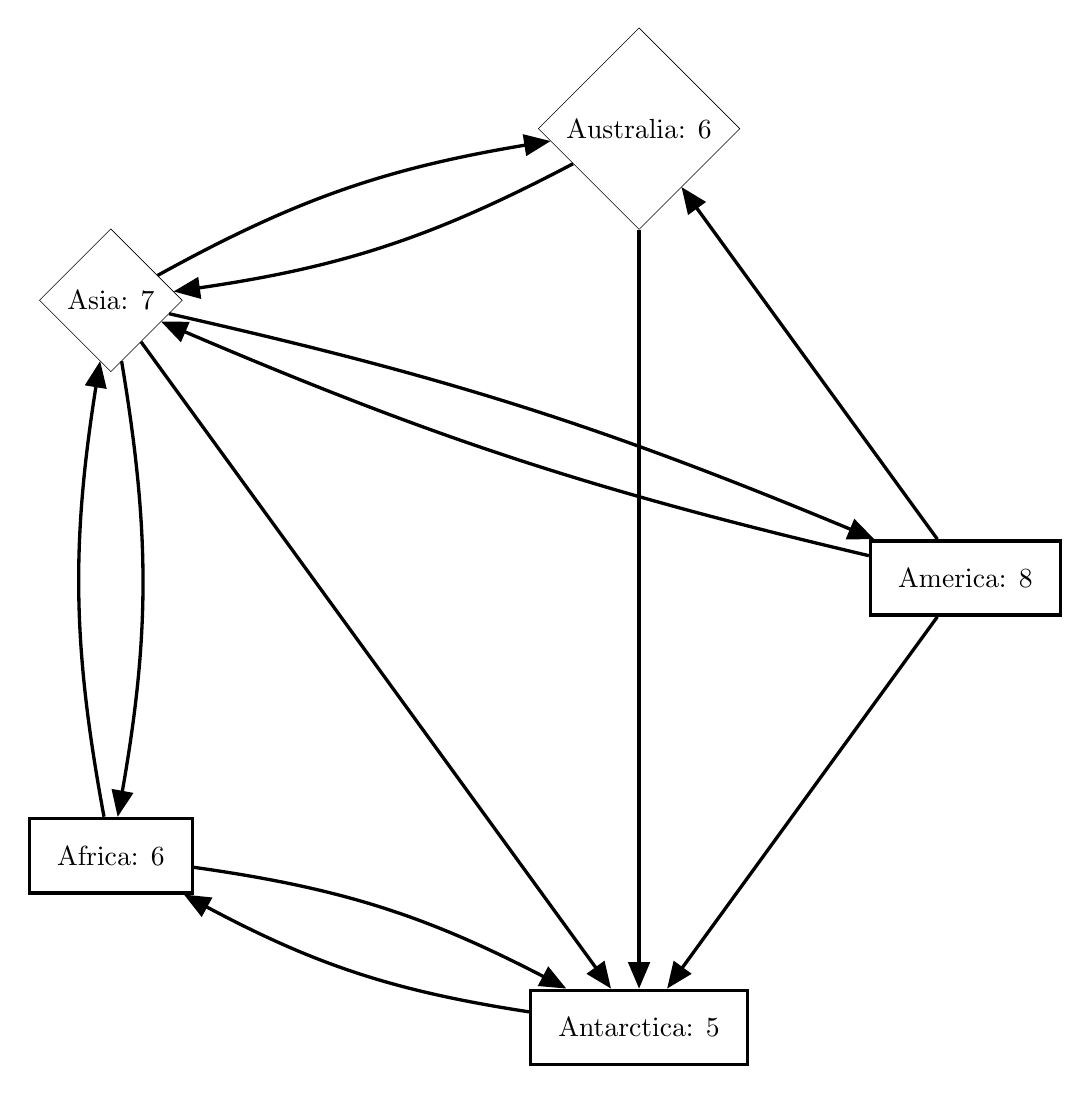
\begin{tikzpicture}[very thick,-triangle 45,start chain=circled placed {at=(\tikzchaincount*72:6)}]

  \tikzstyle{boxnode}=[draw=black,shape=rectangle,inner sep=10pt]
  \tikzstyle{diamnode}=[draw=black,very thin,shape=diamond]

  \node[on chain,diamnode] (australia)  {Australia: 6};
  \node[on chain,diamnode] (asia)       {Asia: 7};
  \node[on chain,boxnode]  (africa)     {Africa: 6};
  \node[on chain,boxnode]  (antarctica) {Antarctica: 5};
  \node[on chain,boxnode]  (america)    {America: 8};

  \path (america)    edge                (australia)
                     edge [bend left=5]  (asia)
                     edge                (antarctica)
        (australia)  edge [bend left=10] (asia)
                     edge                (antarctica)
        (antarctica) edge [bend left=10] (africa)
        (africa)     edge [bend left=10] (antarctica)
                     edge [bend left=10] (asia)
        (asia)       edge [bend left=10] (australia)
                     edge [bend left=5]  (america)
                     edge [bend left=10] (africa)
                     edge                (antarctica);
\end{tikzpicture}}
\end{center}

\caption{An example of a parity game.}
\label{fig:examplegame}
\end{figure}

\begin{example}
\label{ex:examplegame}
The parity game depicted in Fig.~\ref{fig:examplegame} can, for example, be specified as follows.
\begin{verbatim}
     parity 4;
     1 3 0 1,3,4 "Europe";
     0 6 1 4,2 "Africa";
     4 5 1 0 "Antarctica";
     1 8 1 2,4,3 "America";
     3 6 0 4,2 "Australia";
     2 7 0 3,1,0,4 "Asia";
\end{verbatim}
Nodes belonging to player $0$ are shown in diamond shape, the others in box shape. The label in each
node is composed of the node's name and its priority. Note that symbolic names are optional.
\end{example}

Currently, parity games are stored as arrays of node specifications. The index in that array at which
a node is stored, equals its identifier. This has two important and noteworthy consequences.
\begin{itemize}
\item As noted above, using identifiers multiply leads to overriding of nodes. If the parity game
      contains more than one node specification with the same identifier then the \emph{last} node
      specification determines the properties of the node with that index.
\item The size of the array that is allocated to store a parity game is always $n+1$ where $n$ is
      the maximal identifier occurring in the game's specification. To avoid unnecessary waste of
      space you should ensure that the nodes' identifiers in a parity game occupy a closed interval
      of the natural numbers of the form $\{0,1,2,\ldots,n\}$.
\end{itemize}



%%% Local Variables:
%%% mode: latex
%%% TeX-master: "main"
%%% End:

\section{Viewing Parity Games}
\label{sec:viewing}

\pgsolver can display parity games in two different ways: textually and graphically. The former
can be invoked using the command-line option \texttt{-f}.
\begin{verbatim}
    ~/proj/pgsolver> bin/pgsolver -f 
\end{verbatim}
This results in a simple reprinting of the parity game to be solved at the end of \pgsolver's usual
output. The format is the same as the input format described in the previous section.

In order to display parity games graphically one needs the \texttt{graphviz} package, available for
free from
\begin{verbatim}
    http://www.graphviz.org/
\end{verbatim}
\pgsolver can create output in the \texttt{dot}-format which can be displayed using \texttt{dotty} from
the \texttt{graphviz} package for example. The relevant command-line parameter is \texttt{-d} with
a filename which tells \pgsolver to write the \texttt{dot} code into that file after solving the game.
Beware that you need to tell \pgsolver explicitly (how) to solve the game. If you omit this, \pgsolver
will parse the input but not solve the game. However, this can be used to display the game as it is.
\begin{verbatim}
    ~/proj/pgsolver> bin/pgsolver -d graph.dot tests/test1.gm
\end{verbatim}
Then, in order to view it, try
\begin{verbatim}
    ~/proj/pgsolver> dotty graph.dot
\end{verbatim}
\pgsolver can also display a game together with the winning information. This happens when you tell it
to create \texttt{dot}-code for the game \emph{and} tell it to solve it.
\begin{verbatim}
    ~/proj/pgsolver> bin/pgsolver -global recursive -d graph.dot tests/test1.gm
\end{verbatim}
Again, the result can be viewed using
\begin{verbatim}
    ~/proj/pgsolver> dotty graph.dot
\end{verbatim}
for example. However, now nodes and some edges are coloured according to the following specification.
\begin{itemize}
\item The winning region for player $0$, i.e.\ all nodes from which he/she can win the game, is coloured 
      green. The winning region for player $1$ is coloured red.
\item An edge coloured green belongs to the positional strategy for player $0$ that is winning on his/her
      winning region. An edge coloured red belongs to player $1$'s respective winning strategy.
\end{itemize}
An example display of a solved parity game is given on the title page.



%%% Local Variables: 
%%% mode: latex
%%% TeX-master: "main"
%%% End: 

\section{Additional Tools}
\label{sec:tools}

\subsection{Obfuscator}

This tool randomly permutes the identifiers of nodes as well as the order
of nodes' successors in a parity game. This is useful to confuse algorithms
which perform very well on certain benchmarks because of the order in which
nodes and successors are given.

\begin{example}
Take the ladder game of index 4, as introduced in Sect.~\ref{sec:laddergame}
below. In \pgsolver's specification format it looks like this.
\begin{verbatim}
    ~/pgsolver> bin/laddergame 4
    parity 7;
    0 0 0 1,2;
    1 1 1 2,3;
    2 0 0 3,4;
    3 1 1 4,5;
    4 0 0 5,6;
    5 1 1 6,7;
    6 0 0 7,0;
    7 1 1 0,1;
\end{verbatim}
Each player owns 4 out of the eight nodes. Since all nodes have outdegree 2, there
are $2^4 = 16$ strategies for each of the player. In general, there are $2^n$
different strategies in the game of index $n$ but only one of them is
a winning strategy. However, the winning strategy for player $0$ for example is
an obvious one in this case. It consists of always choosing the first node in the
list of successors. Equally, the winning strategy for player $1$ consists of always
choosing the last node in each list. This is hardly a good hiding of the winning
strategies.

Obfuscator employs a random generator to destroy the order of the successors and
the order in which the nodes are given. A typical obfuscation of the ladder game of
index 4 would be the following.
\begin{verbatim}
    ~/pgsolver> bin/laddergame 4 | bin/obfuscator
    parity 7;
    0 1 1 6,1;
    1 1 1 7,5;
    2 1 1 3,0;
    3 0 0 0,6;
    4 0 0 2,3;
    5 1 1 4,2;
    6 0 0 1,7;
    7 0 0 5,4;
\end{verbatim}
\end{example}

Obfuscator is automatically built through \verb#make obfuscator#,
\verb#make tools#, or \verb#make all#.
It takes a parity game on \texttt{stdin} in the specification format described above
and returns the permuted game on \texttt{stdout}. The currently understood command-line
parameters are:
\begin{description}
\item[{\tt --disablenodeobfuscation}] \enspace or {\tt -dn} \\
	Disables the obfuscation of the ordering of nodes.

\item[{\tt --disableedgeobfuscation}] \enspace or {\tt -de} \\
    Disables the obfuscation of the ordering of the edges.
\end{description}



\subsection{Compressor}

This tool compresses a given parity game s.t.\ the winning sets and strategies of
the resulting game equal those of the original game.

\begin{example}
Take the Jurdzi{\'n}ski game of $J_{1, 2}$, as introduced in Sect.~\ref{sec:jurdgame} below.
In \pgsolver's specification format it looks like this.
\begin{verbatim}
    ~/pgsolver> bin/jurdzinskigame 1 2
    parity 11;
    0 1 0 5;
    2 1 0 7;
    4 2 1 5,0;
    6 2 1 5,7,2;
    5 2 0 4,6,9;
    7 2 0 7,6;
    8 4 0 9;
    10 4 0 9,11;
    9 3 1 8,10,5;
    11 3 1 10,11,7;
\end{verbatim}
It is possible to push priorities along edges overriding smaller priorities. It is also possible
to reassign priorities just keeping parities and the order inbetween them. This leads to the
following game:
\begin{verbatim}
    ~/pgsolver> bin/jurdzinskigame 1 2 | bin/compressor -pr -pp
    parity 11;
    0 0 0 5;
    2 0 0 7;
    4 0 1 5,0;
    5 0 0 4,6,9;
    6 0 1 5,7,2;
    7 0 0 7,6;
    8 2 0 9;
    9 1 1 8,10,5;
    10 2 0 9,11;
    11 1 1 10,11,7;
\end{verbatim}
It is also possible to compress the original game's identifier space eliminating unused node indetifiers.
\begin{verbatim}
    ~/pgsolver> bin/jurdzinskigame 1 2 | bin/compressor --nodes
    parity 9;
    0 1 0 3;
    1 1 0 5;
    2 2 1 3,0;
    3 2 0 2,4,7;
    4 2 1 3,5,1;
    5 2 0 5,4;
    6 4 0 7;
    7 3 1 6,8,3;
    8 4 0 7,9;
    9 3 1 8,9,5;
\end{verbatim}
Note that the original game does not possess a node called $1$ for instance.
\end{example}

Compressor is automatically built through \verb#make compressor#,
\verb#make tools#, or \verb#make all#. It takes a parity game in the specification format described above
on \texttt{stdin} or from a given file, and returns the compressed game on \texttt{stdout}. The currently
understood command-line parameters are:
\begin{description}
\item[\nonterminal{filename}] \ \\
   Tells the tool to look for the specification of the parity game to transform in the file
   \nonterminal{filename}.

\item[{\tt --priorities}] \enspace or {\tt -pr} \\
    It reduces the priority of each node preserving their parities as well as the relation $\le$
    among priorities of nodes within an SCC of the game graph.

\item[{\tt --priopropagation}] \enspace or {\tt -pp} \\
    It tries to reduce the overall number of priorities occurring in the game by pushing priorities
    along edges of the game graph overriding smaller ones. If all nodes leading to a node $v$ have a
    greater priority than the node itself, the priority of this node is altered to the least predecessing
    priority. Similarly the priority of a node is adapted if all successors of a node have a greater
    priority than the node itself. This process is iterated until stability is reached.

    Obviously, this process may destroy the preservation of parities and the less-or-equals relation among
    priorites described above.

\item[{\tt --antipropagation}] \enspace or {\tt -ap} \\
	It tries to set the priority of as many nodes as possible to zero. If all nodes leading to a node
	$v$ have a greater priority than the node itself, the priority of this node can be set to zero.
	Similarly the priority of a node is adapted if all successors of a node have a greater priority than
	the node itself. This process is iterated until stability is reached.

\item[{\tt  --fakealt}] \enspace or {\tt -fa} \\
    Keep fake alternation w.r.t.\ priorities. If this option is enabled the compaction of priorities
    never assigns the same priority to nodes that had different priorities before, even if there is
    no other priority occurring inbetween and both priorities in question are of the same parity.

\item[{\tt --wholegame}] \enspace or {\tt -pp} \\
    The compression of priorities is usually done independently for each SCC of the game graph.
    This switch causes the graph's SCC decomposition to be ignored. This will in general result
    in a worse compression rate.

\item[{\tt --nodes}] \enspace or {\tt -no} \\
    Performs a compression of the space of identifiers of a parity game, resulting in a possible
    down-shift of identifiers.

\item[{\tt --minmaxswap}] \enspace or {\tt -mm} \\
    Transforms a min-parity game into a max-parity one and vice versa.
\end{description}


\subsection{Combinator}

This tool combines two or more parity games into one single parity game by shifting the node numbers.
Neither additional edges between the games are added nor other modifications are done.

\begin{example}
We just create two small random games and combine them to see what happens.
\begin{verbatim}
    ~/pgsolver> bin/randomgame 5 5 2 3 | tee game1.gm
    parity 4;
    0 1 1 3,4 "0";
    1 4 0 1,4 "1";
    2 5 0 0,2,4 "2";
    3 1 0 0,2,4 "3";
    4 0 1 0,1,3 "4";

    ~/pgsolver> bin/randomgame 5 5 2 3 | tee game2.gm
    parity 4;
    0 4 0 2,3 "0";
    1 5 0 0,4 "1";
    2 4 1 0,2,3 "2";
    3 4 0 2,4 "3";
    4 4 1 0,3 "4";
\end{verbatim}
A combination of both games can be achieved as follows:
\begin{verbatim}
    ~/pgsolver> bin/combine game1.gm game2.gm
    parity 9;
    0 1 1 3,4 "0";
    1 4 0 1,4 "1";
    2 5 0 0,2,4 "2";
    3 1 0 0,2,4 "3";
    4 0 1 0,1,3 "4";
    5 4 0 7,8 "0";
    6 5 0 5,9 "1";
    7 4 1 5,7,8 "2";
    8 4 0 7,9 "3";
    9 4 1 5,8 "4";
\end{verbatim}
\end{example}

Combine is automatically built through \verb#make combine#,
\verb#make tools#, or \verb#make all#.
It takes arbitrarly many parity games as command-line parameters and returns the
combined game on \texttt{stdout}. There are no other command-line parameters.


\subsection{Transformer}

This tool transforms a given parity game into an (somehow) equivalent parity game fulfilling
certain properties -- depending on the user's command line specification. The transformed
parity game can be associated with the original game s.t.\ winning sets and strategies can
be easily back-transformed.

% Additionally, winning strategies in the transformed game can be canonically identified with winning strategies in the original game: the totality
% transformation essentially connects nodes with out-degree 0 with themselves and the choice-alternation transformation replaces all edges between
% nodes belonging to the same player with dummy transfer nodes belonging to the other player.

\begin{example}
Again, take the ladder game of index 3, as introduced in Sect.~\ref{sec:laddergame} below.
In \pgsolver's specification format it looks like this.
\begin{verbatim}
    ~/pgsolver> bin/laddergame 3
    parity 5;
    0 0 0 1,2;
    1 1 1 2,3;
    2 0 0 3,4;
    3 1 1 4,5;
    4 0 0 5,0;
    5 1 1 0,1;
\end{verbatim}
The game is obviously total but not choice-alternating as node $0$ is directly connected to node $2$
with both of them belonging to player $0$. A choice-alternation version of this game can obtained as follows:
\begin{verbatim}
    ~/pgsolver> bin/laddergame 3 | bin/transformer --alternating
    parity 11;
    0 0 0 1,6;
    1 1 1 2,7;
    2 0 0 3,8;
    3 1 1 4,9;
    4 0 0 5,10;
    5 1 1 0,11;
    6 0 1 2;
    7 0 0 3;
    8 0 1 4;
    9 0 0 5;
    10 0 1 0;
    11 0 0 1;
\end{verbatim}
\end{example}

Transformer is automatically built through \verb#make transformer#,
\verb#make tools#, or \verb#make all#.
It takes a parity game in the specification format described above on \texttt{stdin} or from a file,
and returns the transformed game on \texttt{stdout}. The currently understood command-line parameters are:

\begin{description}
\itemsep3mm
\item[\nonterminal{filename}] \ \\
   Tells the tool to look for the specification of the parity game to transform in the file
   \nonterminal{filename}.

\item[{\tt --total}] \enspace or {\tt -to} \\
   Perform a totality transformation on the given parity game.

\item[{\tt --alternating}] \enspace or {\tt -al} \\
   Perform a choice-alternation transformation on the given parity game.

 \item[{\tt --singlescc}] \enspace or {\tt -scc} \\
   Perform a simple transformation that results in a single-scc-parity game. The winning sets and
   strategies of the original game and the transformed game match.

 \item[{\tt --prioalignment}] \enspace or {\tt -pa} \\
   Performs a transformation s.t.\ the parity of each node of the resulting game matches its player
   unless its priority is zero.

\item[{\tt --dummynodes}] \enspace or {\tt -dn} \\
   Performs a transformation that divides each edge by an additional node with priority $0$.

\item[{\tt --uniquizeprios}] \enspace or {\tt -up} \\
   Performs a transformation of the occurring priorities s.t.\ every occurring priority occurs only once.

 \item[{\tt --cheapescapecycles}] \enspace or {\tt -ce} \\
   Adds two low-priority cycles $c_0$ and $c_1$ to the game that are profitable for either one of the
   player ($c_0$ for player $0$ and $c_1$ for player $1$). All nodes in the original belonging to
   player $0$ get additional edges leading to $c_1$ and all nodes belonging to player $1$ get
   additional edges leading to $c_0$.

\item[{\tt --bouncingnode}] \enspace or {\tt -bn} \\
   Replaces every self-cycle by a bouncing node.

 \item[{\tt --increasepriorityoccurrence}] \enspace or {\tt -ip} \\
   Increases the occurrence of all priorities by one by simply inserting a long cycle that is not
   connected to the rest of the game.

\item[{\tt --antiprioritycompactation}] \enspace or {\tt -ap} \\
   Adds additional nodes that prohibits any priority compactation.
\end{description}

Note that the command-line parameters that are specified are carried out in the same ordering as they
appear in the call of the transformer tool. It is also possible to specify a parameter more than once.


\subsection{Benchmark Tool}

This tool helps the user to carry out benchmarks and to compare the different solvers with each other. 
You can specify a list of games that are to be benchmarked with a list of solver that also has to be 
specified.

You can either choose to receive a verbose output showing the exact timing of each case or a simple line 
containing data that can be easily parsed by \texttt{gnuplot}. The latter output option is usually to be 
used in combination with a shell script creating a whole benchmark series.

\begin{example}
The following example shows how to benchmark the recursive and the strategy improvement algorithm on a 
random game with 1000 nodes. To smooth multitasking interference factors, each test case is carried out 
3 times.
\begin{verbatim}
    ~/pgsolver> bin/randomgame 1000 1000 2 4 | bin/benchmark -re -si -t 3
    Benchmarking stratimprove...
    Game # 0, Iteration #1...0.02 sec
    Game # 0, Iteration #2...0.02 sec
    Game # 0, Iteration #3...0.02 sec
    Finished. Best: 0.02 sec  Avg: 0.02 sec  Worst: 0.02 sec

    Benchmarking recursive...
    Game # 0, Iteration #1...0.01 sec
    Game # 0, Iteration #2...0.00 sec
    Game # 0, Iteration #3...0.01 sec
    Finished. Best: 0.00 sec  Avg: 0.01 sec  Worst: 0.01 sec

    +-----------------------------------------------------------+
    | Benchmark Statistics                                      |
    +-----------------------------------------------------------+
    | Solver       |         Best |      Average |        Worst |
    +-----------------------------------------------------------+
    | recursive    |     0.00 sec |     0.01 sec |     0.01 sec |
    | stratimprove |     0.02 sec |     0.02 sec |     0.02 sec |
    +-----------------------------------------------------------+
\end{verbatim}
\end{example}

Benchmark is automatically built through \verb#make benchmark#, \verb#make tools#, or \verb#make all#.
It takes one ore more parity games in the specification format described above on \texttt{stdin} or
from files, and carries out the benchmark. The currently understood command-line parameters are:

\begin{description}
\itemsep3mm
\item[\nonterminal{filename}] \ \\
   Tells the tool to look for the specification of the parity game in the file
   \nonterminal{filename}.

\item[{\tt --all}] \enspace or {\tt -a} \\
   Benchmark all available parity games solvers.

\item[{\tt --\nonterminal{solver}}] \ \\
   Benchmark the specified solver. All solvers that are compiled into \pgsolver are available here.

\item[{\tt --silent}] \enspace or {\tt -s} \\
   Only print the final statistics on \texttt{stdout}.

\item[{\tt --gnuplotformat}] \enspace or {\tt -gp} \\
   Only print a gnuplot-compatible line.

 \item[{\tt --timeout \nonterminal{timeout}}] \enspace or {\tt -t \nonterminal{timeout}} \\
   If one of the solvers requires more than $t$ seconds on one of the test cases, the solver is ignored
   for the rest of the series. There is no timeout by default.

\item[{\tt --name \nonterminal{title}}] \enspace or {\tt -n \nonterminal{title}} \\
   Specifies the title of the benchmark that is to be printed in the final statistics.

 \item[{\tt --times \nonterminal{n}}] \enspace or {\tt -t \nonterminal{n}} \\
   Specifies the number of iterations a single test case is carried out per algorithm. By default, $n$
   is 10.

\item[{\tt --\nonterminal{optimisation-option}}] \ \\
   All optimisation options that are available to \texttt{pgsolver} are also available here.
\end{description}



%%% Local Variables:
%%% mode: latex
%%% TeX-master: "main"
%%% End:


\chapter{Benchmarks}
\label{chp:benchmarks}

%\section{Benchmark Games}

The \pgsolver library contains a few programs that create benchmarks for the parity game
solvers. They are built using the command
\begin{verbatim}
    ~/pgsolver> make generators
\end{verbatim}
and reside afterwards in the subdirectory \texttt{bin}.

Additionally, it is possible to compile all generators directly into \pgsolver by setting
the variable \texttt{LINKGENERATORS} to \texttt{YES} in the \texttt{./Config}-file. This
has the advantage that the process of generating and solving a game is not slowed down by
formatting the game first and parsing it afterwards again into the same data structure.

\section{Random Games}

\subsection{A Na\"{\i}ve Model}
Randomly generated parity games are the simplest form of benchmarking utility to assess the
performance of game solvers. The ones used here are parametrized by four parameters: the number
$n$ of nodes in the game, the highest priority $p$, a lower and an upper bound $l$ and $u$ on the
out-degree of each node. The call
\begin{verbatim}
    ~/pgsolver> bin/randomgame 1000 200 2 5
\end{verbatim}
creates a random game with 1000 nodes as follows: for each node $v$,
\begin{itemize}
\item the priority $\Omega(v)$ is uniformly chosen among $\{0,\ldots,200\}$;
\item node $v$ belongs to player $0$ with probability $0.5$ and therefore to player $1$ with
      probability $0.5$ as well;
\item a number $d$ is uniformly chosen in the range $\{2,\ldots,5\}$, and $d$ pairwise different
      nodes are uniformly chosen as $v$'s successors.
\end{itemize}
Beware that \texttt{bin/randomgame} may crash or not terminate if the lower bound on the outdegree
is greater than the upper bound or that one is greater than the number of nodes.


\subsection{Clustered Random Games}

Almost every game created by the random generator above consists of a single big SCC and many adhesive
chains.

Therefore this generator uses an other random model that accomplishes to bring a bit more structure into its instances. It depends on nine parameters: The number of nodes $n$, the highest possibly occurring priority $p$, an out-degree range $(l;h)$, a recursion depth $r$, a recursion breadth range $(a;b)$ and an interconnection range $(x;y)$. An instance of $\mathcal{G}^c_{(n,r)}$ with $c = (p,l,h,a,b,x,y)$ can be generated as follows. If $r = 0$ or $a > n$ simply return a randomly generated game with $n$ nodes, highest priority $p$ and out-degree bounds $l$ and $h$ as above. If $r > 0$ and $a \leq n$,
\begin{itemize}
\item a number $d$ is uniformly chosen in the range $\{a,\ldots,\min(b,n)\}$;
\item $d$ numbers $k_0,\ldots,k_{d-1}$ are uniformly chosen in the range $\{0,\ldots,n-1\}$ s.t.\ $\sum_{i=0}^{d-1} k_i = n$;
\item $d$ instances $G_0,\ldots,G_{d-1}$ are chosen, where $G_i$ is chosen from $\mathcal{G}^c_{(k_i,r-1)}$ (we assume the nodes of all $G_i$ to be pairwise different);
\item a game $G$ is created by the union of all $G_i$;
\item a number $e$ is uniformly chosen in the range $\{x,\ldots,y\}$;
\item $e$ additional uniformly chosen edges in $G$ are added to $G$;
\item the game $G$ is returned.
\end{itemize}

Basically, this recursive approach creates a topological tree structure that is partially intercepted by adding the additional interconnection edges.

A clustered random game with 1000 nodes, highest priority 2, out-degree bounds 2 and 5, recursion depth 3, recursion breadth between 4 and 6 and interconnection degree between 11 and 22 is created using the call
\begin{verbatim}
    ~/pgsolver> bin/clusteredrandomgame 1000 200 2 5 3 4 6 11 22
\end{verbatim}


\subsection{Steady Random Games}

The Steady Random Generator tries to circumvent many universal optimisations in order to particularly
benchmark the backend solvers. The Steady Random Generator is parametrized by five parameters: the number
$n$ of nodes (and different priorities) in the game, a lower and an upper bound and on the
out-degree of each node and a lower and an upper bound and on the in-degree of each node. The call
\begin{verbatim}
    ~/pgsolver> bin/steadygame 1000 2 4 3 5
\end{verbatim}
creates a random game with 1000 nodes as follows: for each node $v$,
\begin{itemize}
\item the priority $\Omega(v)$ is simply $v$;
\item node $v$ belongs to player $0$ with probability $0.5$ and therefore to player $1$ with
      probability $0.5$ as well;
\item a number $d$ is uniformly chosen in the range $\{2,\ldots,4\}$, and $d$ pairwise different
      nodes are uniformly chosen in $v$'s subgame as $v$'s successors;
\item a number $d$ is uniformly chosen in the range $\{3,\ldots,5\}$, and an attempt is made to ensure
      that $v$ has $d$ pairwise different predecessors.
\end{itemize}
All edges are iteratively determined as long as there are at least two different nodes with one of them violating
a lower bound and the other one being below the opposite upper bound uniformly between two such nodes.


\section{Special Graph Structures}

\subsection{Clique Games}

The clique game of order $n$ is $G_n = (\{0,\ldots,n-1\},\{0,2,4,\ldots\},\{1,3,5,\ldots\},E,\Omega)$
with $E = \{ (v,w) \mid v \ne w \}$ and $\Omega(v) = v$. It forms a clique in a directed graph without
self-cycles. Clique games exhibit a large amount of cycles in the game which may pose difficulties
for certain solvers. Note that adding self-cycles to the nodes will result in easy solving because
self-cycles are partial winning strategies in this case, and then all other nodes would lie in the attractor
of these winning regions.

The clique game of order $50$ for instance is generated as follows.
\begin{verbatim}
    ~/pgsolver> bin/cliquegame 50
\end{verbatim}
The clique game of order 50 with self-cycles can also be generated.
\begin{verbatim}
    ~/pgsolver> bin/cliquegame 50 self
\end{verbatim}


\subsection{Ladder Games}
\label{sec:laddergame}

The name of these games is derived from their structure which is reminiscent of a ladder. The
\emph{ladder game} of index $n$ is $G_n = (V,V_0,V_1,E,\Omega)$, defined as follows.
\begin{itemize}
\item $V = \{0,\ldots,2n-1\}$,
\item $V_0 = \{0,2,4,\ldots,2n-2\}$, $V_1 = \{1,3,5,\ldots,2n-1\}$,
\item $E = \{ (v,w) \mid w \equiv_{2n} v+i $ for some $i \in \{1,2\}$ $\}$,
\item $\Omega(v) = v \mod 2$.
\end{itemize}
where $\equiv_{2n}$ means equality modulo $2n$.

It is not hard to see that player $0$ wins on $V_0$ and player $1$ wins on $V_1$ since both can
stay within these regions and only see the priorities $0$, resp.\ $1$.

Ladder games are chosen as benchmarks because in $G_n$ there are $2^n$ many positional strategies for each
player but only one of them is a winning strategy. Not surprisingly, ladder games are very difficult
to solve for the strategy guessing heuristic for example.

The ladder game of index 19 is created using the call
\begin{verbatim}
    ~/pgsolver> bin/laddergame 19
\end{verbatim}


\section{Hard Games for Particular  Algorithms}


\subsection{Jurdzi{\'n}ski Games}
\label{sec:jurdgame}

Jurdzi{\'n}ski has defined a family of games on which the small progress measures algorithm
exhibits an exponential running time \cite{Jurdzinski/00}. The Jurdzi{\'n}ski game $J_{d,w}$ of depth 
$d$ and width $w$ forms a rectangle of dimension $(2d+1) \times (2w)$. For instance, $J_{50,100}$
is generated by calling
\begin{verbatim}
    ~/pgsolver> bin/jurdzinskigame 50 100
\end{verbatim}


% \begin{figure}[t]
% \begin{center}
% \scalebox{0.6}{\input{graphics/marcingame.eepic}}
% \end{center}

% \caption{The Jurdzi{\'n}ski games.}
% \label{fig:marcingame}
% \end{figure}



\subsection{Recursive Ladder Games}

%\newcommand{\playercirc}[3]{
	\pgfcircle[stroke]{\pgfpoint{#1}{#2}}{0.5cm}
	\pgfputat{\pgfpoint{#1}{#2}}{\pgfbox[center,center]{#3}}
}

\newcommand{\playerrect}[3]{
	\pgfrect[stroke]{\pgfrelative{\pgfpoint{#1}{#2}}{\pgfpoint{-0.5cm}{-0.5cm}}}{\pgfpoint{1.0cm}{1.0cm}}
	\pgfputat{\pgfpoint{#1}{#2}}{\pgfbox[center,center]{#3}}
}

\newcommand{\playercircs}[3]{
	\pgfcircle[stroke]{\pgfpoint{#1}{#2}}{0.25cm}
	\pgfputat{\pgfpoint{#1}{#2}}{\pgfbox[center,center]{#3}}
}

\newcommand{\playerrects}[3]{
	\pgfrect[stroke]{\pgfrelative{\pgfpoint{#1}{#2}}{\pgfpoint{-0.25cm}{-0.25cm}}}{\pgfpoint{0.5cm}{0.5cm}}
	\pgfputat{\pgfpoint{#1}{#2}}{\pgfbox[center,center]{#3}}
}

\newcommand{\playeredge}[2]{
	\pgfsetendarrow{\pgfarrowto}
	\pgfline{#1}{#2}
}

\newcommand{\playeredgecurve}[3]{
	\pgfsetendarrow{\pgfarrowto}
	\pgfmoveto{#1}
	\pgfcurveto{#2}{#2}{#3}
	\pgfstroke
}

\newcommand{\playeredgecurvex}[4]{
	\pgfsetendarrow{\pgfarrowto}
	\pgfmoveto{#1}
	\pgfcurveto{#2}{#3}{#4}
	\pgfstroke
}

\newcommand{\playeredgelr}[3]{
	\playeredge{\pgfrelative{\pgfpoint{#1}{#3}}{\pgfpoint{0.5cm}{0.0cm}}}{\pgfrelative{\pgfpoint{#2}{#3}}{\pgfpoint{-0.5cm}{0.0cm}}}
}

\newcommand{\playeredgerl}[3]{
	\playeredge{\pgfrelative{\pgfpoint{#1}{#3}}{\pgfpoint{-0.5cm}{0.0cm}}}{\pgfrelative{\pgfpoint{#2}{#3}}{\pgfpoint{0.5cm}{0.0cm}}}
}

\newcommand{\playeredgeud}[3]{
	\playeredge{\pgfrelative{\pgfpoint{#1}{#2}}{\pgfpoint{0cm}{-0.5cm}}}{\pgfrelative{\pgfpoint{#1}{#3}}{\pgfpoint{0cm}{0.5cm}}}
}

\newcommand{\playeredgedu}[3]{
	\playeredge{\pgfrelative{\pgfpoint{#1}{#2}}{\pgfpoint{0cm}{0.5cm}}}{\pgfrelative{\pgfpoint{#1}{#3}}{\pgfpoint{0cm}{-0.5cm}}}
}

\newcommand{\playeredgeblur}[4]{
	\playeredge{\pgfrelative{\pgfpoint{#1}{#2}}{\pgfpoint{0.35cm}{0.35cm}}}{\pgfrelative{\pgfpoint{#3}{#4}}{\pgfpoint{-0.35cm}{-0.35cm}}}
}

\newcommand{\playeredgeurbl}[4]{
	\playeredge{\pgfrelative{\pgfpoint{#1}{#2}}{\pgfpoint{-0.35cm}{-0.35cm}}}{\pgfrelative{\pgfpoint{#3}{#4}}{\pgfpoint{0.35cm}{0.35cm}}}
}

\newcommand{\playeredgeulbr}[4]{
	\playeredge{\pgfrelative{\pgfpoint{#1}{#2}}{\pgfpoint{0.35cm}{-0.35cm}}}{\pgfrelative{\pgfpoint{#3}{#4}}{\pgfpoint{-0.35cm}{0.35cm}}}
}

\newcommand{\playeredgebrul}[4]{
	\playeredge{\pgfrelative{\pgfpoint{#1}{#2}}{\pgfpoint{-0.35cm}{0.35cm}}}{\pgfrelative{\pgfpoint{#3}{#4}}{\pgfpoint{0.35cm}{-0.35cm}}}
}

\newcommand{\playeredgeselfdn}[2]{\playeredgecurvex{\pgfrelative{\pgfpoint{#1}{#2}}{\pgfpoint{0.16cm}{-0.5cm}}}{\pgfrelative{\pgfpoint{#1}{#2}}{\pgfpoint{0.60cm}{-1.40cm}}}{\pgfrelative{\pgfpoint{#1}{#2}}{\pgfpoint{-0.60cm}{-1.40cm}}}{\pgfrelative{\pgfpoint{#1}{#2}}{\pgfpoint{-0.16cm}{-0.50cm}}}}

\newcommand{\playeredgeselfrs}[2]{\playeredgecurvex{\pgfrelative{\pgfpoint{#1}{#2}}{\pgfpoint{+0.25cm}{0.08cm}}}{\pgfrelative{\pgfpoint{#1}{#2}}{\pgfpoint{+0.7cm}{+0.3cm}}}{\pgfrelative{\pgfpoint{#1}{#2}}{\pgfpoint{+0.7cm}{-0.3cm}}}{\pgfrelative{\pgfpoint{#1}{#2}}{\pgfpoint{+0.25cm}{-0.08cm}}}}

\newcommand{\playeredgecurvelr}[4]{\playeredgecurve{\pgfrelative{\pgfpoint{#1}{#4}}{\pgfpoint{0.5cm}{0.20cm}}}{\pgfrelative{\pgfpoint{#2}{#4}}{\pgfpoint{0cm}{0.5cm}}}{\pgfrelative{\pgfpoint{#3}{#4}}{\pgfpoint{-0.5cm}{0.20cm}}}}

\newcommand{\playeredgecurverl}[4]{\playeredgecurve{\pgfrelative{\pgfpoint{#1}{#4}}{\pgfpoint{-0.5cm}{-0.20cm}}}{\pgfrelative{\pgfpoint{#2}{#4}}{\pgfpoint{0cm}{-0.5cm}}}{\pgfrelative{\pgfpoint{#3}{#4}}{\pgfpoint{0.5cm}{-0.20cm}}}}

\newcommand{\playeredgecurvelrs}[4]{\playeredgecurve{\pgfrelative{\pgfpoint{#1}{#4}}{\pgfpoint{0.25cm}{0.10cm}}}{\pgfrelative{\pgfpoint{#2}{#4}}{\pgfpoint{0cm}{0.25cm}}}{\pgfrelative{\pgfpoint{#3}{#4}}{\pgfpoint{-0.25cm}{0.10cm}}}}

\newcommand{\playeredgecurverls}[4]{\playeredgecurve{\pgfrelative{\pgfpoint{#1}{#4}}{\pgfpoint{-0.25cm}{-0.10cm}}}{\pgfrelative{\pgfpoint{#2}{#4}}{\pgfpoint{0cm}{-0.25cm}}}{\pgfrelative{\pgfpoint{#3}{#4}}{\pgfpoint{0.25cm}{-0.10cm}}}}


\newcommand{\playeredgecurvetd}[4]{\playeredgecurve{\pgfrelative{\pgfpoint{#1}{#2}}{\pgfpoint{-0.20cm}{-.5cm}}}{\pgfrelative{\pgfpoint{#1}{#3}}{\pgfpoint{-.5cm}{0cm}}}{\pgfrelative{\pgfpoint{#1}{#4}}{\pgfpoint{-0.20cm}{.5cm}}}}

\newcommand{\playeredgecurvedt}[4]{\playeredgecurve{\pgfrelative{\pgfpoint{#1}{#2}}{\pgfpoint{0.20cm}{.5cm}}}{\pgfrelative{\pgfpoint{#1}{#3}}{\pgfpoint{.5cm}{0cm}}}{\pgfrelative{\pgfpoint{#1}{#4}}{\pgfpoint{0.20cm}{-.5cm}}}}

\newcommand{\pictrecursiveladder}[0]{
\begin{pgfpicture}{-1cm}{-1.5cm}{10cm}{9cm}
\pgfsetlinewidth{0.7pt}
\playerrect{0cm}{8cm}{$a_0: 1$}
\playercirc{0cm}{6cm}{$b_0: 1$}
\playerrect{0cm}{4cm}{$c_0: 5$}
\playercirc{0cm}{2cm}{$d_0: 4$}
\playerrect{0cm}{0cm}{$e_0: 3$}
\playercirc{3cm}{8cm}{$a_1: 0$}
\playerrect{3cm}{6cm}{$b_1: 0$}
\playercirc{3cm}{4cm}{$c_1: 8$}
\playerrect{3cm}{2cm}{$d_1: 7$}
\playercirc{3cm}{0cm}{$e_1: 6$}
\playerrect{6cm}{8cm}{$a_2: 1$}
\playercirc{6cm}{6cm}{$b_2: 1$}
\playerrect{6cm}{4cm}{$c_2: 11$}
\playercirc{6cm}{2cm}{$d_2: 10$}
\playerrect{6cm}{0cm}{$e_2: 9$}
\playercirc{9cm}{8cm}{$a_3: 0$}
\playerrect{9cm}{6cm}{$b_3: 0$}
\playeredgecurvelr{0cm}{1.5cm}{3cm}{2cm}
\playeredgecurverl{3cm}{1.5cm}{0cm}{2cm}
\playeredgecurvelr{3cm}{4.5cm}{6cm}{2cm}
\playeredgecurverl{6cm}{4.5cm}{3cm}{2cm}
\playeredgecurvetd{0cm}{8cm}{7cm}{6cm}
\playeredgecurvedt{0cm}{6cm}{7cm}{8cm}
\playeredgecurvetd{3cm}{8cm}{7cm}{6cm}
\playeredgecurvedt{3cm}{6cm}{7cm}{8cm}
\playeredgecurvetd{6cm}{8cm}{7cm}{6cm}
\playeredgecurvedt{6cm}{6cm}{7cm}{8cm}
\playeredgecurvetd{9cm}{8cm}{7cm}{6cm}
\playeredgecurvedt{9cm}{6cm}{7cm}{8cm}
\playeredgecurvetd{0cm}{2cm}{1cm}{0cm}
\playeredgecurvedt{0cm}{0cm}{1cm}{2cm}
\playeredgecurvetd{3cm}{2cm}{1cm}{0cm}
\playeredgecurvedt{3cm}{0cm}{1cm}{2cm}
\playeredgecurvetd{6cm}{2cm}{1cm}{0cm}
\playeredgecurvedt{6cm}{0cm}{1cm}{2cm}
\playeredgeud{0cm}{6cm}{4cm}
\playeredgeud{0cm}{4cm}{2cm}
\playeredgeud{3cm}{6cm}{4cm}
\playeredgeud{3cm}{4cm}{2cm}
\playeredgeud{6cm}{6cm}{4cm}
\playeredgeud{6cm}{4cm}{2cm}
\playeredge{\pgfpoint{0.5cm}{0cm}}{\pgfpoint{2.5cm}{5.9cm}}
\playeredge{\pgfpoint{3.5cm}{0cm}}{\pgfpoint{5.5cm}{5.9cm}}
\playeredge{\pgfpoint{6.5cm}{0cm}}{\pgfpoint{8.5cm}{5.9cm}}
\playeredge{\pgfpoint{0.5cm}{4cm}}{\pgfpoint{2.5cm}{6.1cm}}
\playeredge{\pgfpoint{3.5cm}{4cm}}{\pgfpoint{5.5cm}{6.1cm}}
\playeredge{\pgfpoint{6.5cm}{4cm}}{\pgfpoint{8.5cm}{6.1cm}}
\playeredge{\pgfpoint{2.5cm}{8cm}}{\pgfpoint{0.5cm}{2cm}}
\playeredge{\pgfpoint{5.5cm}{8cm}}{\pgfpoint{3.5cm}{2cm}}
\playeredge{\pgfpoint{8.5cm}{8cm}}{\pgfpoint{6.5cm}{2cm}}
\end{pgfpicture}
}




\newcommand{\thegame}[4]{
\newcommand{\declaneeven}{a}
\newcommand{\declaneodd}{b}
\newcommand{\declaneevenroot}{c}
\newcommand{\declaneoddroot}{d}
\newcommand{\cyclenodea}{e}
\newcommand{\cyclenodeb}{f}
\newcommand{\cyclenodec}{g}
\newcommand{\cyclecenter}{h}
\newcommand{\cycleaccess}{k}
\newcommand{\cycleselector}{l}
\newcommand{\cycleleaver}{m}
\newcommand{\upperselector}{z}
\newcommand{\finalsink}{p}
\newcommand{\finalcycle}{q}
\newcommand{\starteven}{s}
\newcommand{\startselector}{t}
\newcommand{\highentrybit}{w}
\newcommand{\lowestbit}{y}
\newcommand{\bitselector}{x}
\begin{pgfpicture}{#1}{#2}{#3}{#4}
\pgfsetlinewidth{0.7pt}
\playercirc{0cm}{2cm}{$\declaneodd_0: 21$}
\playerrect{2cm}{2cm}{$\declaneeven_0: 22$}
\playercirc{0cm}{4cm}{$\declaneodd_1: 23$}
\playerrect{2cm}{4cm}{$\declaneeven_1: 24$}
\playercirc{0cm}{6cm}{$\declaneodd_2: 25$}
\playerrect{2cm}{6cm}{$\declaneeven_2: 26$}
\playercirc{0cm}{8cm}{$\declaneodd_3: 27$}
\playerrect{2cm}{8cm}{$\declaneeven_3: 28$}
\playercirc{0cm}{10cm}{$\declaneodd_4: 29$}
\playerrect{2cm}{10cm}{$\declaneeven_4: 30$}
\playercirc{0cm}{12cm}{$\declaneodd_5: 31$}
\playerrect{2cm}{12cm}{$\declaneeven_5: 32$}
\playercirc{0cm}{14cm}{$\declaneodd_6: 33$}
\playerrect{2cm}{14cm}{$\declaneeven_6: 34$}
\playerrect{2cm}{0cm}{$\declaneevenroot: 35$}
\playercirc{0cm}{0cm}{$\declaneoddroot: 36$}
\playercirc{8cm}{8cm}{$\cyclenodea_0: 9$}
\playercirc{8cm}{14cm}{$\cyclenodea_1: 15$}
\playercirc{6cm}{6cm}{$\cyclenodeb_0: 11$}
\playercirc{6cm}{12cm}{$\cyclenodeb_1: 17$}
\playercirc{8cm}{4cm}{$\cyclenodec_0: 13$}
\playercirc{8cm}{10cm}{$\cyclenodec_1: 19$}
\playerrect{10cm}{6cm}{$\cyclecenter_0: 14$}
\playerrect{10cm}{12cm}{$\cyclecenter_1: 20$}
\playerrect{12cm}{4cm}{$\cycleaccess_0: 41$}
\playerrect{12cm}{10cm}{$\cycleaccess_1: 45$}
\playercirc{16cm}{4cm}{$\cycleselector_0: 10$}
\playercirc{16cm}{10cm}{$\cycleselector_1: 16$}
\playerrect{16cm}{6cm}{$\cycleleaver_0: 42$}
\playerrect{16cm}{12cm}{$\cycleleaver_1: 46$}
\playercirc{18cm}{6cm}{$\upperselector_0: 39$}
\playercirc{18cm}{12cm}{$\upperselector_1: 43$}
\playerrect{20cm}{6cm}{$\finalsink: 48$}
\playerrect{20cm}{4cm}{$\finalcycle: 1$}
\playercirc{13cm}{14cm}{$\lowestbit: 5$}
\playercirc{15cm}{14cm}{$\highentrybit: 7$}
\playercirc{-3cm}{8cm}{$\bitselector: 38$}
\playercirc{8cm}{0cm}{$\starteven: 2$}
\playercirc{-3cm}{6cm}{$\startselector: 3$}
\playeredgerl{2cm}{0cm}{0cm}
\playeredgerl{2cm}{0cm}{2cm}
\playeredgerl{2cm}{0cm}{4cm}
\playeredgerl{2cm}{0cm}{6cm}
\playeredgerl{2cm}{0cm}{8cm}
\playeredgerl{2cm}{0cm}{10cm}
\playeredgerl{2cm}{0cm}{12cm}
\playeredgerl{2cm}{0cm}{14cm}
\playeredgeud{0cm}{2cm}{0cm}
\playeredgeud{0cm}{4cm}{2cm}
\playeredgeud{0cm}{6cm}{4cm}
\playeredgeud{0cm}{8cm}{6cm}
\playeredgeud{0cm}{10cm}{8cm}
\playeredgeud{0cm}{12cm}{10cm}
\playeredgeud{0cm}{14cm}{12cm}
\playeredgelr{10cm}{16cm}{6cm}
\playeredgelr{10cm}{16cm}{12cm}
\playeredgelr{16cm}{18cm}{6cm}
\playeredgelr{16cm}{18cm}{12cm}
\playeredgerl{16cm}{12cm}{4cm}
\playeredgerl{16cm}{12cm}{10cm}
\playeredgeblur{16cm}{4cm}{18cm}{6cm}
\playeredgeblur{16cm}{10cm}{18cm}{12cm}
\playeredgelr{18cm}{20cm}{6cm}
\playeredgeulbr{18cm}{12cm}{20.35cm}{6.17cm}
\playeredgebrul{18cm}{6cm}{16cm}{10cm}
\playeredgeud{20cm}{6cm}{4cm}
\playeredgeselfdn{20cm}{4cm}
% \playeredgebrul{12cm}{4cm}{9.70cm}{5.83cm}
\playeredgebrul{11.87cm}{4.13cm}{9.70cm}{5.83cm}
%\playeredgebrul{12cm}{10cm}{9.70cm}{11.83cm}
\playeredgebrul{11.87cm}{10.13cm}{9.70cm}{11.83cm}
\playeredgebrul{10.35cm}{6.17cm}{8cm}{8cm}
\playeredgebrul{10.35cm}{12.17cm}{8cm}{14cm}
\playeredgeurbl{8cm}{8cm}{6cm}{6cm}
\playeredgeurbl{8cm}{14cm}{6cm}{12cm}
\playeredgeulbr{6cm}{6cm}{8cm}{4cm}
\playeredgeulbr{6cm}{12cm}{8cm}{10cm}
\playeredgeblur{8cm}{4cm}{10.30cm}{5.83cm}
\playeredgeblur{8cm}{10cm}{10.30cm}{11.83cm}
\playeredgecurvelr{13cm}{14cm}{15cm}{14cm}
\playeredgecurverl{15cm}{14cm}{13cm}{14cm}
\playeredgecurvex{\pgfpoint{13cm}{13.5cm}}{\pgfpoint{12cm}{7cm}}{\pgfpoint{15cm}{5cm}}{\pgfpoint{15.65cm}{4.35cm}}
\playeredgecurve{\pgfpoint{15cm}{13.5cm}}{\pgfpoint{14.5cm}{11cm}}{\pgfpoint{15.65cm}{10.35cm}}
\playeredgecurvex{\pgfpoint{15.5cm}{14cm}}{\pgfpoint{17cm}{14.5cm}}{\pgfpoint{19cm}{15cm}}{\pgfpoint{20.25cm}{6.5cm}}
\playeredgecurvex{\pgfpoint{6.45cm}{5.8cm}}{\pgfpoint{7.5cm}{6.5cm}}{\pgfpoint{10.5cm}{3.5cm}}{\pgfpoint{11.5cm}{3.8cm}}
\playeredgecurvex{\pgfpoint{6.45cm}{12.2cm}}{\pgfpoint{7.5cm}{12.5cm}}{\pgfpoint{10.5cm}{9.5cm}}{\pgfpoint{11.5cm}{10.2cm}}
\playeredgecurvex{\pgfpoint{6.45cm}{6.2cm}}{\pgfpoint{11cm}{8cm}}{\pgfpoint{10cm}{9cm}}{\pgfpoint{11.5cm}{9.8cm}}
\playeredgecurvex{\pgfpoint{6.45cm}{11.8cm}}{\pgfpoint{9cm}{12cm}}{\pgfpoint{11.5cm}{6.5cm}}{\pgfpoint{12cm}{4.5cm}}
\playeredgecurvex{\pgfpoint{8.5cm}{0cm}}{\pgfpoint{14cm}{4.5cm}}{\pgfpoint{17cm}{1.5cm}}{\pgfpoint{19.5cm}{5.9cm}}
% \playeredgeblur{8cm}{0cm}{12cm}{4cm}
\playeredgeblur{8cm}{0cm}{11.87cm}{3.87cm}
\playeredgecurve{\pgfpoint{8.45cm}{0.23cm}}{\pgfpoint{14cm}{4cm}}{\pgfpoint{12.45cm}{9.5cm}}
\playeredgecurve{\pgfpoint{8cm}{7.5cm}}{\pgfpoint{9.5cm}{4cm}}{\pgfpoint{8cm}{0.5cm}}
\playeredgecurvex{\pgfpoint{8cm}{13.5cm}}{\pgfpoint{9cm}{11cm}}{\pgfpoint{10.5cm}{3.5cm}}{\pgfpoint{8.2cm}{0.45cm}}
\playeredgecurvex{\pgfpoint{-0.25cm}{1.55cm}}{\pgfpoint{-0.1cm}{-0.6cm}}{\pgfpoint{-4cm}{-1.5cm}}{\pgfpoint{7.54cm}{-0.2cm}}
\playeredgecurvex{\pgfpoint{-0.25cm}{3.55cm}}{\pgfpoint{-0.9cm}{-0.8cm}}{\pgfpoint{-4cm}{-2.0cm}}{\pgfpoint{7.58cm}{-0.25cm}}
\playeredgecurvex{\pgfpoint{-0.25cm}{5.55cm}}{\pgfpoint{-1.7cm}{-1.0cm}}{\pgfpoint{-4cm}{-2.5cm}}{\pgfpoint{7.62cm}{-0.3cm}}
\playeredgecurvex{\pgfpoint{-0.25cm}{7.55cm}}{\pgfpoint{-2.5cm}{-1.2cm}}{\pgfpoint{-4cm}{-3.0cm}}{\pgfpoint{7.66cm}{-0.35cm}}
\playeredgecurvex{\pgfpoint{-0.25cm}{9.55cm}}{\pgfpoint{-3.3cm}{-1.4cm}}{\pgfpoint{-4cm}{-3.5cm}}{\pgfpoint{7.70cm}{-0.40cm}}
\playeredgecurvex{\pgfpoint{-0.25cm}{11.55cm}}{\pgfpoint{-4.1cm}{-1.6cm}}{\pgfpoint{-4cm}{-4.0cm}}{\pgfpoint{7.75cm}{-0.45cm}}
\playeredgecurvex{\pgfpoint{-0.25cm}{13.55cm}}{\pgfpoint{-4.9cm}{-1.8cm}}{\pgfpoint{-4cm}{-4.5cm}}{\pgfpoint{7.80cm}{-0.50cm}}
\playeredge{\pgfpoint{-0.3cm}{0.4cm}}{\pgfpoint{-2.71cm}{7.55cm}}
\playeredge{\pgfpoint{-0.5cm}{2cm}}{\pgfpoint{-2.64cm}{7.64cm}}
\playeredge{\pgfpoint{-0.5cm}{4cm}}{\pgfpoint{-2.58cm}{7.76cm}}
\playeredge{\pgfpoint{-0.5cm}{6cm}}{\pgfpoint{-2.53cm}{7.88cm}}
\playeredge{\pgfpoint{-0.5cm}{8cm}}{\pgfpoint{-2.5cm}{8cm}}
\playeredge{\pgfpoint{-0.5cm}{10cm}}{\pgfpoint{-2.53cm}{8.12cm}}
\playeredge{\pgfpoint{-0.5cm}{12cm}}{\pgfpoint{-2.58cm}{8.24cm}}
\playeredge{\pgfpoint{-0.5cm}{14cm}}{\pgfpoint{-2.64cm}{8.36cm}}
\playeredgedu{-3cm}{6cm}{8cm}
\playeredge{\pgfpoint{-0.5cm}{0cm}}{\pgfpoint{-2.7cm}{5.6cm}}
\playeredgecurvex{\pgfpoint{-3cm}{5.5cm}}{\pgfpoint{-4cm}{-1.8cm}}{\pgfpoint{-2cm}{-4.5cm}}{\pgfpoint{8cm}{-0.5cm}}
\playeredgecurvex{\pgfpoint{-3cm}{8.5cm}}{\pgfpoint{-4cm}{19cm}}{\pgfpoint{8cm}{15cm}}{\pgfpoint{14.7cm}{14.4cm}}
\playeredgecurvex{\pgfpoint{-2.9cm}{8.48cm}}{\pgfpoint{-4cm}{18.5cm}}{\pgfpoint{8cm}{15cm}}{\pgfpoint{12.7cm}{14.4cm}}
\playeredgecurvex{\pgfpoint{7.53cm}{14.1cm}}{\pgfpoint{5cm}{14.2cm}}{\pgfpoint{4.5cm}{11.9cm}}{\pgfpoint{2.5cm}{12cm}}
\playeredgecurvex{\pgfpoint{7.53cm}{10.1cm}}{\pgfpoint{5cm}{10.0cm}}{\pgfpoint{4.5cm}{14.1cm}}{\pgfpoint{2.5cm}{14cm}}
\playeredgecurvex{\pgfpoint{5.53cm}{12.1cm}}{\pgfpoint{4.5cm}{12.2cm}}{\pgfpoint{3.5cm}{9.9cm}}{\pgfpoint{2.5cm}{10cm}}
\playeredgecurvex{\pgfpoint{7.5cm}{10cm}}{\pgfpoint{5cm}{10.2cm}}{\pgfpoint{4.5cm}{7.9cm}}{\pgfpoint{2.5cm}{8.1cm}}
\playeredgecurvex{\pgfpoint{7.53cm}{4.1cm}}{\pgfpoint{5cm}{4.0cm}}{\pgfpoint{4.5cm}{8.1cm}}{\pgfpoint{2.5cm}{7.9cm}}
\playeredgecurvex{\pgfpoint{7.5cm}{14.0cm}}{\pgfpoint{3.5cm}{14.2cm}}{\pgfpoint{4.0cm}{5.9cm}}{\pgfpoint{2.5cm}{6.1cm}}
\playeredgecurvex{\pgfpoint{7.53cm}{8.1cm}}{\pgfpoint{5cm}{8.2cm}}{\pgfpoint{4.5cm}{5.9cm}}{\pgfpoint{2.5cm}{5.9cm}}
\playeredgecurvex{\pgfpoint{6cm}{11.5cm}}{\pgfpoint{6cm}{11cm}}{\pgfpoint{5.0cm}{5cm}}{\pgfpoint{2.5cm}{4.1cm}}
\playeredgecurvex{\pgfpoint{5.5cm}{6cm}}{\pgfpoint{4.5cm}{6.2cm}}{\pgfpoint{3.5cm}{3.9cm}}{\pgfpoint{2.5cm}{3.9cm}}
\playeredgecurvex{\pgfpoint{7.53cm}{9.9cm}}{\pgfpoint{3.5cm}{10.2cm}}{\pgfpoint{4.0cm}{1.9cm}}{\pgfpoint{2.5cm}{2.1cm}}
\playeredgecurvex{\pgfpoint{7.53cm}{3.9cm}}{\pgfpoint{5cm}{4.2cm}}{\pgfpoint{4.5cm}{1.9cm}}{\pgfpoint{2.5cm}{1.9cm}}
\playeredgecurvex{\pgfpoint{7.53cm}{13.9cm}}{\pgfpoint{3.0cm}{14.2cm}}{\pgfpoint{3.5cm}{-0.1cm}}{\pgfpoint{2.5cm}{0.1cm}}
\playeredgecurvex{\pgfpoint{7.53cm}{7.9cm}}{\pgfpoint{3.5cm}{8.2cm}}{\pgfpoint{4.0cm}{-0.1cm}}{\pgfpoint{2.5cm}{-0.1cm}}
\end{pgfpicture}
}

\newcommand{\pictexpstratimpr}{\thegame{0cm}{-1.5cm}{22cm}{14cm}}


\newcommand{\pictmodelcheckerladder}{
\begin{pgfpicture}{-2cm}{-2cm}{12cm}{4cm}
\pgfsetlinewidth{0.7pt}
\playercirc{0cm}{2cm}{$1$}
\playerrect{2cm}{2cm}{$2$}
\playercirc{4cm}{2cm}{$3$}
\playerrect{6cm}{2cm}{$4$}
\playercirc{8cm}{2cm}{$5$}
\playerrect{10cm}{2cm}{$6$}
\playercirc{0cm}{0cm}{$12$}
\playerrect{2cm}{0cm}{$11$}
\playercirc{4cm}{0cm}{$10$}
\playerrect{6cm}{0cm}{$9$}
\playercirc{8cm}{0cm}{$8$}
\playerrect{10cm}{0cm}{$7$}
\playeredgelr{0cm}{2cm}{2cm}
\playeredgelr{2cm}{4cm}{2cm}
\playeredgelr{4cm}{6cm}{2cm}
\playeredgelr{6cm}{8cm}{2cm}
\playeredgelr{8cm}{10cm}{2cm}
\playeredgeud{0cm}{2cm}{0cm}
\playeredgeud{2cm}{2cm}{0cm}
\playeredgeud{4cm}{2cm}{0cm}
\playeredgeud{6cm}{2cm}{0cm}
\playeredgeud{8cm}{2cm}{0cm}
\playeredgeud{10cm}{2cm}{0cm}
\playeredgeblur{0cm}{0cm}{1.85cm}{1.85cm}
\playeredgeblur{2.15cm}{0.15cm}{4cm}{2cm}
\playeredgeblur{4cm}{0cm}{5.85cm}{1.85cm}
\playeredgeblur{6.15cm}{0.15cm}{8cm}{2cm}
\playeredgeblur{8cm}{0cm}{9.85cm}{1.85cm}
\playeredgeud{0cm}{3.5cm}{2cm}
\playeredgelr{-1.5cm}{0cm}{2cm}
\pgfsetendarrow{}
\pgfline{\pgfpoint{10cm}{2.5cm}}{\pgfpoint{10cm}{3cm}}
\pgfline{\pgfpoint{10cm}{3cm}}{\pgfpoint{0cm}{3cm}}
\pgfline{\pgfpoint{10cm}{-0.5cm}}{\pgfpoint{10cm}{-1cm}}
\pgfline{\pgfpoint{10cm}{-1cm}}{\pgfpoint{-1cm}{-1cm}}
\pgfline{\pgfpoint{-1cm}{-1cm}}{\pgfpoint{-1cm}{2cm}}
\end{pgfpicture}
}

% \begin{figure}[t]
% \begin{center}
% \pictrecursiveladder
% \end{center}
% \caption{The recursive ladder game of index 4.}
% \label{fig:recursiveladder}
% \end{figure}

The recursive ladder games form a family on which the recursive algorithm exhibits an exponential
running time.  The recursive ladder game of index $n$ has size $5 \cdot n$. 
% We omit a formal
% definition here. The construction can easily be inferred from Fig.~\ref{fig:recursiveladder}. Inside
% the nodes it shows the node's identifier (left of the colon) and its priority.
The recursive ladder game of index 4 results in 20 nodes and is generated by calling
\begin{verbatim}
    ~/pgsolver> bin/recursiveladder 4
\end{verbatim}





\subsection{Exponential Strategy Improvement Games}

The exponential strategy improvement games form a family on which both strategy improvement algorithms
exhibit an exponential running time (in the index of the game) \cite{FriedmannSI09}.
The exponential strategy improvement game of index $n$ has size $14 \cdot n + 11$. 
% We omit a formal definition here. The game of index 2 is depicted in Fig.~\ref{fig:expstratimpr}.
% Inside the nodes it
%shows the node's identifier (left of the colon) and its priority.
A game of index 4 results in 67 nodes and is generated by calling
\begin{verbatim}
    ~/pgsolver> bin/expstratimpr 4
\end{verbatim}

In order to verify that the strategy iteration indeed requires exponential runtime on these games, you
need to either disable all generic optimisations or transform the game using the \texttt{transformer}
tool with the parameters \texttt{-ss -ap -bn}.


% \begin{landscape}
% % \pagenumbering{none}
% \begin{figure}[t]
% \begin{center}
% \pictexpstratimpr
% \end{center}
% \caption{The exponential strategy improvement game of index 2.}
% \label{fig:expstratimpr}
% \end{figure}
% \end{landscape}



\subsection{Model Checker Ladder Games}

The model checker ladder games form a family on which the model checker algorithm exhibits an
exponential running time.  The model checker ladder game of index $n$ has size $4 \cdot n$. 
% We omit a formal definition here. The construction can easily be inferred from
% Fig.~\ref{fig:modelcheckerladder}.
%Inside the nodes it shows the node's identifier (left of the colon) and its priority.
A model checker ladder game of index 3 results in 12 nodes and is generated by calling
\begin{verbatim}
    ~/pgsolver> bin/modelcheckerladder 3
\end{verbatim}

% \begin{figure}[h]
% \begin{center}
% \pictmodelcheckerladder
% \end{center}
% \caption{The model checker ladder game of index 3.}
% \label{fig:modelcheckerladder}
% \end{figure}


\section{Verification Problems}

\subsection{Fairness of an Elevator System}

We encode a simple fairness verification problem as a parity game. States of a transition system modelling
an \emph{elevator} for $n$ floors are of type
$\{1,\ldots,n\} \times \{\mathtt{o},\mathtt{c}\} \times (\bigcup \{ \mathit{Perm}(S) \mid S \subseteq \{1,\ldots,n\})$.
The first component describes the current position of the elevator as one of the floors. The
second component indicates whether the door is \emph{open} or \emph{closed}. The third component -- a permutation
of a subset of all available floors -- holds the \emph{requests}, i.e.\ those floors that should be served next.
The transitions on these are as follows.
\begin{itemize}
\item At any moment, any request or none can be issued. For simplicity reasons, we assume that at most one floor
      is added to the requests per transition. Note that nondeterministically, no request can be issued, and a
      request for a certain floor that is already contained in the current requests does not change them.
\item If the door is open then it is closed in the next step, the current floor does not change.
\item If it is closed, the elevator moves one floor (up or down) into the direction of the first request. If the
      floor reached that way is among the requested ones, the door is opened and that floor is removed from the
      current requests. Otherwise, the door remains closed.
\end{itemize}
We consider two different implementations of this elevator model: the first one stores requests in FIFO
style, the second in LIFO style. The games $G_n$ (with FIFO), resp.\ $G'_n$ (with LIFO) result from
encoding the model checking problem for this transition system and the CTL$^*$ formula
$\mathtt{A}(\mathtt{GF}\mathit{isPressed} \to \mathtt{GF}\mathit{isAt})$ as a parity game
\cite{Stirling95}.  Proposition $\mathit{isPressed}$ holds in any state s.t.\ the request list contains
the number $n$, and $\mathit{isAt}$ holds in a state where the current floor is $n$. Hence, this
formula requires all runs of the elevator to satisfy the following fairness property: if the top floor
is requested infinitely often then it is being served infinitely often. It can easily be formulated in
the modal $\mu$-calculus using a formula of size $11$ and alternation depth $2$ (of type
$\nu$--$\mu$--$\nu$). Hence the resulting parity games have constant index 3.  Note that $G_n$
encodes a positive instance of the model checking problem whereas $G'_n$ encodes a negative one.
The game $G_4$ is generated by calling
\begin{verbatim}
    ~/pgsolver> bin/elevators 4
\end{verbatim}
and the game $G'_5$ by calling
\begin{verbatim}
    ~/pgsolver> bin/elevators -u 5
\end{verbatim}


\section{Particular Problems Encoded as Parity Games}

\subsection{Towers of Hanoi}

The Towers of Hanoi problem can be seen as a reachability game in the graph of game configurations.
The problem of size $n$ has $n$ disks that are to be moved from the first to the third rod.
A problem of size $3$ is generated by calling
\begin{verbatim}
    ~/pgsolver> bin/towersofhanoi 3
\end{verbatim}


\subsection{Language Inclusion Between an NBA and a DBA}

Let $n,m \ge 2$, $\Sigma_n = \{a_1,\ldots,a_n\}$ and consider the language $L_{n,m}$ of all words over the alphabet
$\Sigma_n$ that contain infinitely many occurrences of $(a_i)^m$ for some $i \{ 1,\ldots,n\}$. This language is 
accepted by the following NBA $\mathcal{A}_{n,m}$.
\begin{center}
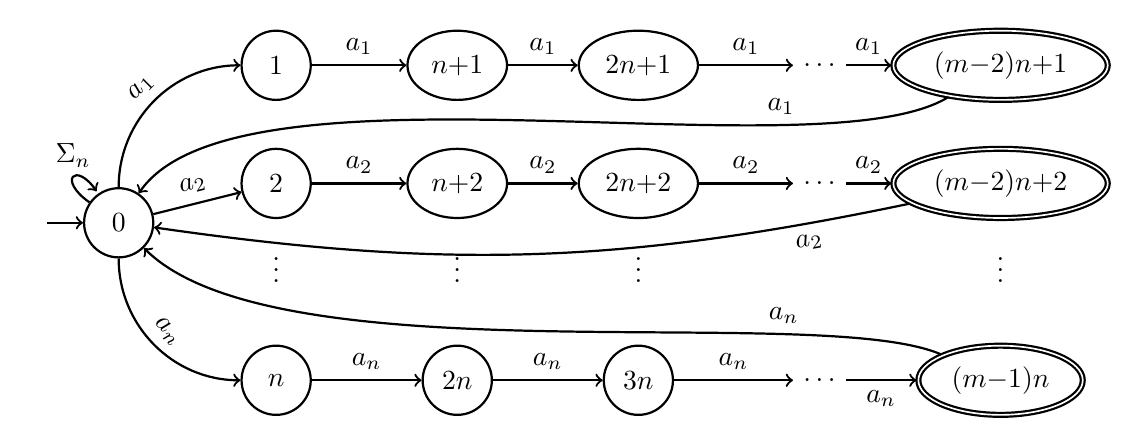
\begin{tikzpicture}[thick,->,initial text={},every state/.style={shape=ellipse}, node distance=2.3cm]
  \node[state,initial]   (0)                    {$0$};
  \node[state]           (1) at ($(0)+(2,2)$)   {$1$};
  \node[state]           (n1) [right of=1]      {$n{+}1$};
  \node[state]           (2n1) [right of=n1]    {$2n{+}1$};
  \node                  (d1) [right of=2n1]    {$\ldots$};
  \node[state,accepting] (m2n1) [right of=d1]   {$(m{-}2)n{+}1$};
  \node[state]           (2) at ($(0)+(2,.5)$) {$2$};
  \node[state]           (n2) [right of=2]      {$n{+}2$};
  \node[state]           (2n2) [right of=n2]    {$2n{+}2$};
  \node                  (d2) [right of=2n2]    {$\ldots$};
  \node[state,accepting] (m2n2) [right of=d2]   {$(m{-}2)n{+}2$};
  \node[state]           (n) at ($(0)+(2,-2)$)  {$n$};
  \node[state]           (2n) [right of=n]      {$2n$};
  \node[state]           (3n) [right of=2n]     {$3n$};
  \node                  (dn) [right of=3n]    {$\ldots$};
  \node[state,accepting] (m1n) [right of=dn]   {$(m{-}1)n$};

  \node (ds1) at ($(0)+(2,-.5)$) {$\vdots$};
  \node (ds2) [right of=ds1] {$\vdots$};
  \node (ds3) [right of=ds2] {$\vdots$};
  \node (ds4) [right of=ds3] {};
  \node ()    [right of=ds4] {$\vdots$};

  \path (0)    edge [out=145,in=125,loop] node [above]                   {$\Sigma_n$} ()
               edge [out=90,in=180]     node [above,sloped]            {$a_1$}      (1)
               edge              node [above,sloped]            {$a_2$}      (2)
               edge [out=270,in=180]             node [above,sloped]            {$a_n$}      (n)
        (1)    edge              node [above]                   {$a_1$}      (n1)
        (n1)   edge              node [above]                   {$a_1$}      (2n1)
        (2n1)  edge              node [above]                   {$a_1$}      (d1)
        (d1)   edge              node [above]                   {$a_1$}      (m2n1)
        (2)    edge              node [above]                   {$a_2$}      (n2)
        (n2)   edge              node [above]                   {$a_2$}      (2n2)
        (2n2)  edge              node [above]                   {$a_2$}      (d2)
        (d2)   edge              node [above]                   {$a_2$}      (m2n2)
        (m2n2) edge [bend left=10]  node [very near start,sloped,below] {$a_2$}      (0)
        (n)    edge              node [above]                   {$a_n$}      (2n)
        (2n)   edge              node [above]                   {$a_n$}      (3n)
        (3n)   edge              node [above]                   {$a_n$}      (dn)
        (dn)   edge              node [below]                   {$a_n$}      (m1n);
%        (m1n)  edge              node [near start,sloped,above] {$a_n$}      (0);

  \draw[->] (m2n1) .. controls ($(m2n1)+(-2.3,-1.4)$) and ($(0)+(1.5,2.2)$) .. (0) node [near start,above] {$a_1$};
  \draw[->] (m1n) .. controls ($(m1n)+(-2.3,1)$) and ($(0)+(2,-2)$) .. (0) node [near start,above] {$a_n$};
\end{tikzpicture}
\end{center}
It is also accepted by the following deterministic B\"uchi automata $\mathcal{B}_{n,m}$.
\begin{center}
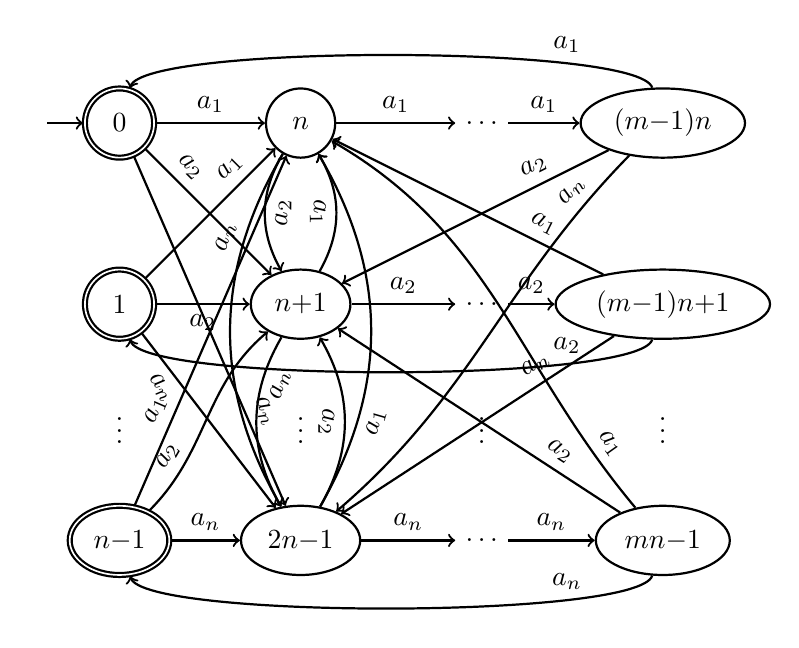
\begin{tikzpicture}[thick,->,node distance=2.3cm,initial text={},every state/.style={shape=ellipse}]
  \node[state,initial,accepting] (0)                        {$0$};
  \node[state,accepting]         (1)      [below of=0]      {$1$};
  \node                          (d1)     [below of=1,node distance=1.5cm]      {$\vdots$}; 
  \node[state,accepting]         (nm1)    [below of=d1,node distance=1.5cm]     {$n{-}1$};
  \node[state]                   (n)      [right of=0]      {$n$};
  \node[state]                   (np1)    [below of=n]      {$n{+}1$};
  \node                          (d2)     [below of=np1,node distance=1.5cm]    {$\vdots$}; 
  \node[state]                   (2nm1)   [below of=d2,node distance=1.5cm]     {$2n{-}1$};
  \node                          (d3)     [right of=n]      {$\ldots$};
  \node                          (d4)     [right of=np1]    {$\ldots$};
  \node                          (d5)     [right of=d2]     {$\vdots$};
  \node                          (d6)     [right of=2nm1]   {$\ldots$};
  \node[state]                   (mm1n)   [right of=d3]     {$(m{-}1)n$};
  \node[state]                   (mm1np1) [below of=mm1n]   {$(m{-}1)n{+}1$};
  \node                          (d7)     [below of=mm1np1,node distance=1.5cm] {$\vdots$}; 
  \node[state]                   (mnm1)   [below of=d7,node distance=1.5cm]     {$mn{-}1$};

  \path[->] (0)    edge node [above] {$a_1$} (n)
            (n)    edge node [above] {$a_1$} (d3)
            (d3)   edge node [above] {$a_1$} (mm1n)
            (1)    edge node [below] {$a_2$} (np1)
            (np1)  edge node [above] {$a_2$} (d4)
            (d4)   edge node [above] {$a_2$} (mm1np1)
            (nm1)  edge node [above] {$a_n$} (2nm1)
            (2nm1) edge node [above] {$a_n$} (d6)
            (d6)   edge node [above] {$a_n$} (mnm1);

  \path[->] (0)      edge                       node [sloped,above,near start]      {$a_2$} (np1)
            (n)      edge [bend right]          node [sloped,below]                 {$a_2$} (np1)
            (mm1n)   edge                       node [sloped,above,near start]      {$a_2$} (np1)
            (1)      edge                       node [sloped,above,near end]        {$a_1$} (n)
            (np1)    edge [bend right]          node [sloped,below]                 {$a_1$} (n)
            (mm1np1) edge                       node [sloped,above,near start]      {$a_1$} (n)
            (0)      edge                       node [sloped,above,near end]        {$a_n$} (2nm1)
            (n)      edge [bend right]          node [sloped,above,near start]        {$a_n$} (2nm1)
            (mm1n)   edge [bend right=5,in=170] node [sloped,above,very near start] {$a_n$} (2nm1)
            (nm1)    edge                       node [sloped,above,near start]      {$a_1$} (n)
            (2nm1)   edge [bend right]          node [sloped,below,near start]      {$a_1$} (n)
            (mnm1)   edge [in=-30,out=130]      node [sloped,above,very near start] {$a_1$} (n)
            (1)      edge                       node [sloped,below,near start]      {$a_n$} (2nm1)
            (np1)    edge [bend right]          node [sloped,below,near start]        {$a_n$} (2nm1)
            (mm1np1) edge                       node [sloped,above,near start]      {$a_n$} (2nm1)
            (nm1)    edge [in=220]              node [sloped,above,near start]      {$a_2$} (np1)
            (2nm1)   edge [bend right]          node [sloped,below]                 {$a_2$} (np1)
            (mnm1)   edge                       node [sloped,above,near start]      {$a_2$} (np1);
            
  \draw[->] (mm1n) .. controls ($(mm1n)+(-.3,1)$) and ($(0)+(.3,1)$) .. (0) node [near start,above] {$a_1$};
  \draw[->] (mm1np1) .. controls ($(mm1np1)+(-.3,-1)$) and ($(1)+(.3,-1)$) .. (1) node [near start,above] {$a_2$};
  \draw[->] (mnm1) .. controls ($(mnm1)+(-.3,-1)$) and ($(nm1)+(.3,-1)$) .. (nm1) node [near start,above] {$a_n$};
\end{tikzpicture}
\end{center}
The synchronous product of $\mathcal{A}_{n,m}$ and $\mathcal{B}_{n,m}$ is a parity game $\mathcal{G}_{n,m}$ in which
every node is owned by player $1$, and the priority of a node $(q,p)$ is given as
\begin{displaymath}
\Omega(q,p) \enspace = \enspace \begin{cases}
2 &,\text{if } p \text{ is accepting,} \\
1 &,\text{if } p \text{ is not accepting and } q \text{ is accepting,} \\
0 &,\text{otherwise.}
\end{cases}
\end{displaymath}
This is the standard encoding of fair simulation as a parity condition \cite{HenzingerKR02,HutagalungLL:LATA13}. This game
encodes the language inclusion problem between an NBA and a DBA. In this case, the game is entirely won by player $0$.

The game $\mathcal{G}_{6,9}$ is generated by
\begin{verbatim}
    ~/pgsolver> bin/langincl 6 9
\end{verbatim}
The second parameter is optional. If it is not given then $m=2$ is chosen by default.

%%% Local Variables:
%%% mode: latex
%%% TeX-master: "main"
%%% End:

%\section{Comparison of the Solvers}



%%% Local Variables: 
%%% mode: latex
%%% TeX-master: "main"
%%% End: 


\chapter{Developer's Guide}
\label{chp:dguide}

\label{chp:devguide}

The purpose of this chapter is to provide enough insight into the structure
of the \pgsolver tool such that it becomes possible to extend it with a new algorithm.
We assume reasonable OCaml programming skills and some familiarity with parity games, though.

Implementing a new algorithm requires two steps only.
\begin{enumerate}
\item Create an OCaml source code file that contains the solver. This is just a function
      which takes a parity game and returns a partition of (a subset of) its node set into
      winning regions and winning strategies for the two players. It must reside in a new
      module.
\item Integrate this function into the main program such that the new solver can be used
      by giving \pgsolver a certain command-line argument. Then adjust the
      \texttt{SolverList} such that the new module is compiled with the rest of the tool.
\end{enumerate}


\section{Structure of the Source Code}

In the following, all references to files are given relatively to the directory into which
\pgsolver was unpacked during the installation process. There, the subdirectory \texttt{src}
is the important one for this step. It contains the source files of all the modules that
make up the \pgsolver library. They are organised into the following subdirectories respectively.
Note that, when we speak of \emph{modules} we often refer to files only that implicitly count as
a module in OCaml.
\begin{description}
\item[\texttt{generators}] contains modules that make up the benchmark generators;
\item[\texttt{tools}] contains tools for the creation or manipulation of parity games;
\item[\texttt{paritygame}] contains modules that define parity games as a data structure and
     provide functionality for that, e.g.\ in the form of procedures that compute SCC decompositions
     etc.;
\item[\texttt{pgsolver}] contains modules for the actual program \texttt{pgsolver};
\item[\texttt{solvers}] contains the parity game solvers, each in a separate module.
\end{description}

\section{Data Types and Functions for Manipulating Parity Games}

The signature file
\begin{verbatim}
src/paritygame/paritygame.mli
\end{verbatim}
contains the definition of parity games as an abstract data structure.
A parity game is internally stored as an array of node definitions but this may or may not change in the future
in favour of a more efficient implementation. There are also (abstract) data types for representing nodes, players,
priorities, sets of nodes, strategies, solutions and solutions, which will be introduced in detail in the following.

\subsection{Nodes}

The type of a node in a paritygame is one of the few types that are not abstract. For sake of efficiency, a node is 
simply an integer value:
\begin{verbatim}
   type node = int
\end{verbatim}
Beware that the type node may become abstract in the future, so try to avoid to arithmetic etc.\ on nodes. 

There is currently only one function that is specific to nodes; it turns a node into a string for output purposes.
\begin{verbatim}
   val nd_show : node -> string
\end{verbatim}


\subsection{Sets of Nodes}

Many algorithms manipulate sets of nodes, for instance they take the set of all nodes with highest priority etc. For 
such purposes, \verb#paritygame.mli# provides an abstract data type and functions for storing and manipulating sets of nodes.
\begin{verbatim}
   type nodeset
\end{verbatim}
Currently, this type is implemented as a simple ordered list without duplicates. The functions for creation and manipulation
follow the standard \verb#Set# interface. Use
\begin{verbatim}
   val ns_empty   : nodeset
   val ns_make    : node list -> nodeset
\end{verbatim}
to create a set of nodes, either initially empty or from a given list of nodes. It is possible to add nodes to existing sets
or deletes nodes from them using
\begin{verbatim}
   val ns_add     : node -> nodeset -> nodeset
   val ns_del     : node -> nodeset -> nodeset
\end{verbatim}
In the latter case \verb#ns_del v vs# returns vs if \verb#v# is not a member of \verb#vs#.

Desctruction of node sets is implemented as 
\begin{verbatim}
   val ns_nodes   : nodeset -> node list
\end{verbatim}
which returns all the elements of a set of nodes as a list.

For tests on emptiness and on membership of a particular node in a set use
\begin{verbatim}
   val ns_isEmpty : nodeset -> bool
   val ns_elem    : node -> nodeset -> bool
\end{verbatim}
There are more general tests, for instance if a node set includes some node with a particular property, or if all of them do so:
\begin{verbatim}
   val ns_exists  : (node -> bool) -> nodeset -> bool			
   val ns_forall  : (node -> bool) -> nodeset -> bool			
\end{verbatim}
It is possible to extract nodes from a node set, either some with a particular property (\verb#ns_find#) or a random one (\verb#ns_some#)
or the first, resp.\ last in some canonical order (\verb#ns_first#, \verb#ns_last#), or the one that is maximal w.r.t.\ a total order
(\verb#ns_max#).
\begin{verbatim} 
   val ns_find    : (node -> bool) -> nodeset -> node
   val ns_some    : nodeset -> node
   val ns_first   : nodeset -> node
   val ns_last    : nodeset -> node
   val ns_max     : nodeset -> (node -> node -> bool) -> node
\end{verbatim}
The cardinality of a set of nodes is computed by
\begin{verbatim}
   val ns_size    : nodeset -> int
\end{verbatim}
Finally, there are the typical iterator functions 
\begin{verbatim}
   val ns_fold    : ('a -> node -> 'a) -> 'a -> nodeset -> 'a
   val ns_iter    : (node -> unit) -> nodeset -> unit
   val ns_map     : (node -> node) -> nodeset -> nodeset
   val ns_filter  : (node -> bool) -> nodeset -> nodeset
\end{verbatim}
that behave as one would expect. Note that there is no control over the order in which nodes in a set are processed in \verb#ns_iter f vs# 
or \verb#ns_fold f x vs#; hence for a uniquely determined result the function \verb#f# should be independent of that order. 


\subsection{Players and Priorities}

There are two types representing players and priorities.
\begin{verbatim}
   type player 
   type priority = int
\end{verbatim}
Players are abstract but priorities are just integers. Only non-negative integers should be used as priorities.

There are constants defining the two players of a parity game. Some algorithms may have to defer the decisio about who wins which node in a game;
for such cases there is also a constant representing an undefined player. At last, there is a function which can be used to obtain a random player
with even distribution between \verb#plr_Even# and \verb#plr_Odd#.
\begin{verbatim} 
   val plr_Even   : player
   val plr_Odd    : player
   val plr_undef  : player
   val plr_random : unit -> player
\end{verbatim}
There are a few functions realising some minor arithmetic on the data type \verb#player#, for instance computing a player's opponent, for obtaining
a string representation, or for applying a function to both players.
\begin{verbatim}
   val plr_opponent : player -> player
   val plr_show     : player -> string
   val plr_iterate  : (player -> unit) -> unit
\end{verbatim}
There are some functions that link players and priorities, for instance by checking whether a priority is good for some player in the sense that
even priorities are good for \verb#plr_Even# and odd ones for \verb#plr_Odd#. Likewise it is possible to obtain the benefitting player directly.
\begin{verbatim}
   val prio_good_for_player : priority -> player -> bool
   val plr_benefits         : priority -> player
\end{verbatim}
These functions essentially test the parity of an integer value; there are also functions to do this directly. 					
\begin{verbatim}
   val odd: priority -> bool
   val even: priority -> bool
\end{verbatim}
It is unlikely, yet not impossible, that the type \verb#priority# will become abstract in the future. Hence, it is advisable to only manipulate
priorities through these functions.


\subsection{Parity Games}
\label{sec:paritygamesmodule}

The most important type in this module is the data type for parity games.
\begin{verbatim}
   type paritygame
\end{verbatim}
Note that as of version 4.0, the implementation of this type is no longer visible to the other modules, for reasons of code reliability. There are,
however, several functions that allow parity games to be created, manipulated and used.

There are three ways for creating a fresh parity game. 
\begin{verbatim}
   val pg_create : int -> paritygame
   val pg_init   : int -> 
                   (node -> (priority * player * node list * string option)) -> 
                   paritygame
   val pg_copy   : paritygame -> paritygame
\end{verbatim}
The former two expect the number of nodes of the game as a parameter. In case of \verb#pg_create#, the resulting game has no edges, the owner of each node
is \verb#plr_undef# and the priorities cannot be assumed to be non-negative integer values. The second function can be used to create a game and
fill it with some structure. Calling \verb#pg_init n f# will return a parity game with \verb#n# nodes such that the result of calling \verb#f i#
contains the priority, owner, list of successor nodes and possibly a name of the \verb#i#-th node in the game. Function \verb#pg_copy# creates a fresh
copy of an existing game which may be handy for algorithms that manipulate games and have to revert certain changes.

Given a parity game, such information about a node can be extracted using the following functions.
\begin{verbatim}
   val pg_get_priority     : paritygame -> node -> priority
   val pg_get_owner        : paritygame -> node -> player
   val pg_get_successors   : paritygame -> node -> nodeset
   val pg_get_predecessors : paritygame -> node -> nodeset
\end{verbatim}
It is possible to search for the node name (as an integer, resp.\ value of type \verb#node#) given its description.
\begin{verbatim}
   val pg_find_desc  : paritygame -> string option -> node
\end{verbatim}
There are two function for finding nodes according to their priorities.
\begin{verbatim}
   val pg_prio_nodes              : paritygame -> priority -> node list
   val pg_get_selected_priorities : paritygame -> 
                                    (priority -> bool) -> 
                                    priority list
\end{verbatim}
A parity game can be modified inplace by setting, resp.\ changing the priority or string description or owner of a node, or by adding an 
edge between two nodes.
\begin{verbatim}
   val pg_set_priority : paritygame -> node -> priority -> unit
   val pg_set_owner    : paritygame -> node -> player -> unit
   val pg_get_desc     : paritygame -> node -> string option
   val pg_set_desc     : paritygame -> node -> string option -> unit
   val pg_get_desc'    : paritygame -> node -> string
   val pg_set_desc'    : paritygame -> node -> string -> unit
   val pg_add_edge     : paritygame -> node -> node -> unit
\end{verbatim}
It is also possible to delete a set of nodes given as a list, or to remove a single edge or a set of edges, given as a list of node pairs. These
deletions also work inplace.
\begin{verbatim}
   val pg_remove_nodes : paritygame -> node list -> unit
   val pg_del_edge     : paritygame -> node -> node -> unit
   val pg_remove_edges : paritygame -> (node * node) list -> unit
\end{verbatim}
Note that using any of these can result in a game in which a node has no successor anymore. Deleting undefined nodes or non-existing edges results
in no change.

Some structural information about a parity game can be obtained, namely the size (i.e.\ number of nodes), the number of edges, or the index (i.e.\ number
of different priorities). 
\begin{verbatim}
   val pg_size	         : paritygame -> int
   val pg_node_count     : paritygame -> int
   val pg_edge_count     : paritygame -> int
   val pg_get_index      : paritygame -> int
   val pg_get_priorities : paritygame -> priority list
\end{verbatim}
The latter returns a list of all the priorities that are being used in the game.

There is a subtle difference between \verb#pg_size# and \verb#pg_node_count#. The latter only counts nodes that are defined, so for instance
\verb#pg_size (pg_create 2)# will return \verb#2#, while \verb#pg_node_count (pg_create 2)# will return \verb#0#. Checking whether a node is defined
can be done using
\begin{verbatim}
   val pg_isDefined : paritygame -> node -> bool
\end{verbatim}
Finally, there are iterator functions for parity games that traverse through all defined nodes, resp.\ all existing edges.
\begin{verbatim}
  val pg_iterate      : (node -> 
                         (priority * player * nodeset * nodeset * string option) -> 
                         unit) -> paritygame -> unit
  val pg_edge_iterate : (node -> node -> unit) -> paritygame -> unit
\end{verbatim}

\subsection{Solutions and Strategies}

A solution of a parity game is a mapping of nodes to players, determining who wins the game starting in that particular node.
A (memory-less) strategy (for both players) is a set of edges, including exactly one edge for each node that is won by the
player who owns the node. The interface \verb#paritygame.mli# provides two data structures for solutions and strategies which are
based on the fact that nodes are non-negative integer values.
\begin{verbatim}
   type solution = player array
   type strategy = node array
\end{verbatim}
A solution with value \verb#plr_Even# at position \verb#v# for instance represents the fact that player Even wins node \verb#v#.
Such arrays can contain the value \verb#plr_undef#.

An array of type \verb#strategy# can contain the value \verb#nd_undef#, representing the fact that the strategy decision at that position
is either unknown or unnecessary because the node is not won by its owner.

Note that an array of type \verb#strategy# contains, in effect, two positional strategies -- one for each player.

There is no mechanism that links a solution or strategy array to a particular parity game. It is the programmer's task to ensure
that the solution for one game is not used for another game. This could result in runtime errors like array access outside their
bounds.

\section{Implementing a New Solver}

We will exemplarily describe how to implement and integrate a new algorithm that solves parity games. There
is more than one way to do so but there is a unique easiest way which we will follow here.

Suppose you have finally come up with a deterministic polynomial time algorithm. Surely this cannot miss in
the \pgsolver library. It is also quite probable that the algorithm is complex -- for otherwise someone
else would have found it before. Therefore you cannot wait for us to implement it. By the time we have
understood all the algorithm's subtleties our programming skills will have bitten the dust. In that case you
better do it yourself.

Find an expressive name for your algorithm that will be used to create a module and also later a command-line
parameter for the \texttt{pgsolver} program. Say \emph{Deterministic Polynomial Time Solver} was a good name.
Then create two files in the \texttt{src/solvers} subdirectory, for example called
\begin{verbatim}
detpoly.ml
detpoly.mli
\end{verbatim}
The signature file \texttt{detpoly.mli} must look like this.
\begin{verbatim}
val solve : Paritygame.paritygame ->
              Paritygame.solution * Paritygame.strategy
\end{verbatim}
The name of the function is actually irrelevant, but calling it \texttt{solve} is not a bad idea. Its type
is mandatory though. It must take a parity game and return a pair of a solution and a strategy using the
data types described above.

Now sit down and hack the code for the implementation of your solver into the file \texttt{detpoly.ml}. In the
simplest form this will look like
\begin{verbatim}
open Paritygame ;;
let solve game = ...
\end{verbatim}
However, note that this function will be called in the main program, and as the argument \texttt{game} it will
receive the parity game from the input. Hence, this does not automatically make use of the universal solver
described in Sect.~\ref{sec:universal}. This is because one cannot guarantee that the universal optimisations
compression, SCC decomposition and solving of special cases speed up \emph{any} solver.

If your algorithm turns out to be that quick you might not want the universal optimisations in which case you
can skip the following description of how to employ the universal solver with your new algorithm as a backend
and continue with the next section.

So you are still with us -- thanks for the trust you have in our universal solver! Now, you will still have
to implement your algorithm in a function of type
\texttt{Paritygame.paritygame -> Paritygame.solution * Paritygame.strategy} but it may be better to choose
a different name. For instance, create a function
\begin{verbatim}
let my_solver game = ...
\end{verbatim}
in \texttt{detpoly.ml} that contains the implementation of your solver. This may now assume that the argument
\texttt{game} consists of a single SCC only such that the priorities of at least two nodes have different
parities and it is not just one player who has real choices in all the nodes in this game.

Now all you have to do is to make sure that the \texttt{solve}-function declared in \texttt{detpoly.mli}
calls the universal solver using your solver as a backend. This is easily done, \texttt{detpoly.ml} should
look like this.
\begin{verbatim}
let solve = Univsolve.universal_solve
             (Univsolve.universal_solve_init_options_verbose
              !Univsolve.universal_solve_global_options)
              my_solver
\end{verbatim}
Note that, if your solver implemented in \verb#my_solver# is recursive, it can also call \verb#solve# instead
of \verb#my_solver# recursively in order to have the universal optimisations done in every step.


\section{Integrating the New Solver}

Continuing with the example of the previous section we assume that you have implemented a solver in the file
\texttt{src/solvers/detpoly.ml}. In particular, this file contains a function \texttt{solve} of type
\texttt{Paritygame.paritygame -> Paritygame.solution * Paritygame.strategy} which is declared in
\texttt{src/solvers/detpoly.mli}.

You will have to ensure that your file does automatically get compiled when \pgsolver is being built using
the \texttt{make} command. In \texttt{SolverList} you will find a variable declaration listing all the modules
that make up the entire program. It should look like this.
\begin{verbatim}
PGSOLVERSLIST=
	obj/recursive.cmx \
	obj/stratimprovement.cmx \
	...
	obj/stratimprlocal.cmx \
	obj/stratimprdisc.cmx 
\end{verbatim}
Append to this list \texttt{obj/detpoly.cmx}. It need not be at the end of this list but you have to make
sure that it occurs behind any other module that contains code which is used by your solver. This could
be the \texttt{paritygame} and \texttt{univsolve} part for example and will most certainly be the
\texttt{solvers} part. Now running \texttt{make} should compile the \texttt{detpoly}-module as well.

At last, you have to integrate your algorithm into the program so that it can be used through the
\texttt{pgsolver} program when given a certain command-line option. This could not be an easier. Add to
your file \texttt{detpoly.ml} the following code after your \texttt{solve} function.
\begin{verbatim}
let _ = Solvers.register_solver
          solve
          "detpoly"
          "dp"
          "use the brand-new deterministic polytime algorithm"
\end{verbatim}
The function \texttt{register\_solver} from the module \texttt{solvers.ml} does everything for you. You
simply have to give it four arguments.
\begin{itemize}
\item The first one, here \texttt{solve} is the function of the type described above that implements
      your algorithm.
\item The second one is a string which should contain a concise but reasonably expressive synonym for your
      algorithm. It must not contain white spaces because it will be prefixed by two dashes ``\texttt{--}''
      and used as a command-line parameter that tells \pgsolver to use your algorithm.
\item The third one is a string which contains an even shorter synonym for your algorithm. It will be
      prefixed by a single dash symbol ``\texttt{-}'' and used as a command-line parameter for \texttt{pgsolver}
      with the same effect.
\item The fourth argument is again a string which contains a description of what \pgsolver does
      when given any of the the command-line parameters derived from the second or third argument.
\end{itemize}
After compilation, called \texttt{bin/pgsolver --help} should result in output containing the following
lines.
\begin{verbatim}
PGSolver Collection Ver. 4.0: Parity Game Solver
Authors: Oliver Friedmann (University of Munich) and Martin Lange (University of Kassel), 2008-2016
http://tcsprojects.org

Usage: pgsolver [options] [infile]
Solves the parity game given in <infile>. If this argument is omitted it
reads a game from STDIN.

Options are
  ...
  --globallysolve, -global <solver>
     solves globally, valid solvers are ... detpoly ...
  ...
\end{verbatim}
Finally, calling \texttt{bin/pgsolver -global detpoly} will solve a parity game using your algorithm.



\section{Useful Functions}

When designing a new solver you may need some functionality that other solvers rely on as well. In that
case there is a good chance that one of the modules already contains the function you are looking for,
and you do not have to re-implement it. In the following we describe some of the implemented functions
that are most likely to be useful for solving parity games in general. All path names are relative to
the subdirectory \texttt{src}, i.e.\ when we speak about module \texttt{Basics} in the \texttt{paritygame}
directory for example then this can be found in the file \texttt{src/paritygame/basics.ml}.

%\paragraph{Basics Module}
\subsection{The {\ttfamily Basics} Module}

The main function in this module in the subdirectory \texttt{pgsolver} is used for producing output 
messages to \texttt{STDOUT} during a run of \pgsolver depending on the configured verbosity level.

\begin{description}
\itemsep3mm
\item \verb+type verbosity_level = int+\ \\
Used to define different levels of verbosity during the program's execution.

\item \verb+val message : verbosity_level -> (unit -> string) -> unit+ \ \\
Calling \verb+message v (fun _ -> s)+ outputs the string \verb+s+ on \texttt{STDOUT} if the currently
set verbosity level is greater than or equal to \verb+v+.

\item \verb+val verbosity_level_verbose : verbosity_level+ \ \\
Predefined verbosity level constant for verbose output (2).

\item \verb+val verbosity_level_default : verbosity_level+ \ \\
Predefined verbosity level constant for debug output (3).
\end{description}


\subsection{The {\ttfamily Paritygame} Module}

In addition to the basic functions for creating, accessing and manipulating parity games that have been described in
Section~\ref{sec:paritygamesmodule} already, this module in the \texttt{paritygame} subdirectory contains more useful 
routines for handling parity games. 

\begin{description}
\itemsep3mm
\item \verb+val print_game : paritygame -> unit+ \ \\
Calling \verb+print_game game+ prints game on \texttt{STDOUT} s.t.\ it could be parsed again.

\item \verb+val pg_max_prio : paritygame -> priority+ \ \\
Calling \verb+pg_max_prio game+ returns the greatest priority occurring in the \verb+game+.

\item \verb+val pg_min_prio : paritygame -> priority+ \ \\
Calling \verb+pg_min_prio game+ returns the least priority occurring in the \verb+game+.

\item \verb+val pg_max_prio_for : paritygame -> player -> priority+ \ \\
Calling \verb+pg_max_prio_for game player+ returns the greatest reward for \verb+player+ occurring in the \verb+game+.

\item \verb+val collect_max_prio_nodes : paritygame -> node list+ \ \\
Calling \verb+collect_max_prio_nodes game+ returns all nodes with greatest priority.

\item \verb+val subgame_by_list : paritygame -> node list -> paritygame+ \ \\
Calling \verb+subgame_by_list game nodes+ returns a compressed subgame induced and ordered by the \verb+nodes+-list

\item \verb+val merge_strategies_inplace : strategy -> strategy -> unit+ \ \\
Calling \verb+merge_strategies_inplace strat1 strat2+ adds all strategy decisions from \verb+strat2+ to
\verb+strat1+. Throws an \verb+Unmergable+-Exception if the intersection of the domains of both strategies is not empty, i.e.\ if
there is an index $i$ such that the values of \verb+strat1+ and \verb+strat2+ at index $i$ are both not
\verb#nd_undef#.

\item \verb+val merge_solutions_inplace : solution -> solution -> unit+ \ \\
Calling \verb+merge_solutions_inplace sol1 sol2+ adds all solution information from \verb+sol2+ to \verb+sol1+.
Throws an \verb+Unmergable+-Exception if the intersection of the domains of both solutions is not empty, see above.

\item
\begin{verbatim}
val strongly_connected_components: paritygame ->
                                      (node list array *
                                       scc array *
                                       scc list array *
                                       scc list)
\end{verbatim}
Calling \verb+strongly_connected_components game+ decomposes the \verb+game+ into its SCCs. It returns a tuple
\verb+(sccs, sccindex, topology, roots)+ where \verb+sccs+ is an array mapping each SCC to its list of nodes,
\verb+sccindex+ is an array mapping each node to its SCC (represented by an integer value), \verb+topology+ is an
array mapping each SCC to the list of its immediate successing SCCs and \verb+roots+ is the list of SCC having no
predecessing SCCs. The type \verb#scc# is (currently) just a synonym for \verb#int#. 

\item
\begin{verbatim}
val attr_closure_inplace: paritygame -> strategy ->
                          player -> node list -> node list
\end{verbatim}
Calling \verb+attr_closure_inplace game strategy player region returns+ the attractor for the given \verb+player+
and \verb+region+. Additionally all necessary strategy decisions for \verb+player+ leading into the \verb+region+
are added to \verb+strategy+.

\end{description}


\subsection{The {\ttfamily Univsolve} Module}

This module in the \texttt{paritygame} subdirectory contains the universal solver and some possibly helpful functions
for the universal solving process:
\begin{description}
\itemsep3mm

\item
\begin{verbatim}
val universal_solve :
  universal_solve_options -> (paritygame -> solution * strategy) ->
      paritygame -> solution * strategy
\end{verbatim}
Calling \verb+universal_solve verbosity solver game+ starts the universal solving process using \verb+solver+ as a
backend. It returns the solved game as a pair of \verb+solution+ and \verb+strategy+.

\item
\begin{verbatim}
val universal_solve_by_player_solver :
  universal_solve_options ->
      (paritygame -> player -> solution * strategy) ->
      paritygame -> solution * strategy
\end{verbatim}
Calling \verb+universal_solve_by_player_solver verbosity player_solver game+ \linebreak starts the universal
solving process using \verb+player_solver+ as a backend. Instead of a solver backend that solves arbitrary SCCs
\verb+player_solver+ is supposed to solve an SCC w.r.t.\ a given player, for instance if \verb+player_solver scc plr_Even+
is called, the backend is supposed to determine whether a node is won by player $0$ (return \verb#plr_Even# for this node) or
not (return \verb#plr_undef# for this node). The strategy that is returned by \verb+player_solver+ is only considered w.r.t.\
the given player. The function returns the solved game as a pair of \verb+solution+ and \verb+strategy+.

\item
\begin{verbatim}
val universal_solve_trivial :
   verbosity_level -> paritygame -> solution * strategy
\end{verbatim}
Calling \verb+universal_solve_trivial verbosity game+ starts the universal solving process with a trivial i.e.\
not-solving backend. This function is legal to be called when \verb+game+ can be completely solved by the universal
solving process without requiring the backend. Calling \verb+universal_solve_trivial+ returns the solved game as a
pair of \verb+solution+ and \verb+strategy+.

\item
\begin{verbatim}
val compute_winning_nodes :
   verbosity_level -> paritygame -> strategy -> player -> node list
\end{verbatim}
Calling \verb+compute_winning_nodes verbosity game strategy player+ considers \linebreak the subgame of \verb+game+ w.r.t.\
the \verb+strategy+ decisions for \verb+player+; the strategy is assumed to be total w.r.t.\ \verb+player+. It
returns the list of nodes \verb+player+ wins on the game following \verb+strategy+.
\end{description}
In all these cases the argument \verb+verbosity+ is used to determine whether or not statistics should be printed
at the end.

\section{Creating New Benchmarks}

\subsection{The Functor \texttt{Build}}
The creation of new families of parity games, for example as new benchmarks, is eased by the functor \texttt{Build} in
\texttt{paritygame.mli}. It automates the creation of the necessary data structures for a parity game and allows the
user to specify such a game freely, using their own data types for nodes. In order to do so, one has to implement the
signature
\begin{verbatim}
  module type PGDescription =
    sig
      type gamenode

      val compare    : gamenode -> gamenode -> int

      val owner      : gamenode -> player
      val priority   : gamenode -> priority
      val successors : gamenode -> gamenode list   (* should always return a non-empty list *)
      val show_node  : gamenode -> string option

      val initnodes  : unit -> gamenode list 
    end
\end{verbatim}
i.e.\ create a module that implements some data type \verb#gamenode# and functions which determine the owner and the
priority of a node as well as its successors. Additionally, one has to provide a function that potentially yields a
textual representation of a node, used for instance in displaying a game graphically. Finally, the function \verb#initnodes#
should return a list of initial nodes in such a parity game. 

The \verb#compare# function needs to provide a total order on nodes. It typically suffices to implement it generically via
\verb#let compare = compare#.

Applying the functor \verb#Build# to a module of type \verb#PGDescription# results in a module of type
\begin{verbatim}
  module type PGBuilder = 
    sig
      type gamenode
	     
      val build            : unit -> paritygame
      val build_from_node  : gamenode -> paritygame
      val build_from_nodes : gamenode list -> paritygame
    end
\end{verbatim}
i.e.\ a module which provides functions that build a parity game, either starting generically from the initial nodes as 
defined by the function \verb#initnodes#, or specifically from a particular node or node list. The game is created by 
traversing its description starting at the chosen nodes and exploring successors successively. The user has to guarantee
that the description yields a finite game; otherwise the \verb#build#-functions may not terminate.

The total order given by \verb#compare# is needed to store the nodes of the game description in a hash table or balanced
tree where they are implicitly converted into values of type \verb#node#.

Examples of how to use the functor \verb#Build# for conveniently building parity games on-the-fly can be found in the
\texttt{generators}-subdirectory, for example in the benchmark modules \texttt{towersofhanoi}, \texttt{elevatorverification},
\texttt{jurdzinskigame}, \texttt{langincl}, etc.

\subsection{Registering New Generators}

The modules for benchmarks typically only provide a function that creates a parity game as a value of type \verb#paritygame#.
They do not call the functions themselves, nor are they concerned with where the resulting parity games are being used.

These functions are then used in two places: the most visible one is through the module \texttt{rungenerator} in the 
\texttt{pgsolver} subdirectory. It calls the corresponding function and then prints the resulting game on standard output.
This code is used to create the stand-alone binaries for benchmark creation in the \texttt{bin}-subdirectory.

Printing games and parsing games is very costly, so it is not advisable to use this method to run serious benchmarks. It is
also obviously wasteful to create a paritygame in the correct data type, print it and then parse it again into this data type.
This is why \pgsolver provides a way of integrating the benchmark creation into the main program. This means that games only
need to be created once before they can be solved, without the need to print and parse them. The key to this is the function
\begin{verbatim}
   val register_generator: (string array -> paritygame) -> string -> string -> unit
\end{verbatim}
in the \texttt{generators} module in the subdirectory \texttt{paritygame}. It takes as first argument a function which 
produces a parity game according to an array of strings which are the command-line parameters given to the generator. The
two other arguments of type \verb#string# are a short (i.e.\ not containing white spaces) description of the benchmark,
used to identify this when telling \pgsolver which benchmark to use, and a long description used for instance in the help
text. 

To integrate your benchmarks fully, create a function \verb#my_generator# of type \verb#string array -> paritygame# that returns a 
parity game in accordance to a parameter array (for instance conveniently using the functor \verb#Build#), and include
code of the form
\begin{verbatim}
   let _ = Generators.register_generator my_generator "mygen" "My own benchmark generator"
\end{verbatim}
somewhere, preferably in the same module as the one containing the benchmark generation code. Say its name is \verb#mygenerator#.
To ensure that this code is included in the main program during compilation, you need to add \verb#mygenerator.gen# in the
list of generators in \verb#Makefile#.



%%% Local Variables:
%%% mode: latex
%%% TeX-master: "main"
%%% End:


%\appendix

%\chapter{New Algorithms}
%\label{app:newalg}



\cleardoublepage
\pdfbookmark{Bibliography}{bibliography}
\bibliographystyle{alpha}
\bibliography{./literature}

\end{document}



%%% Local Variables:
%%% mode: latex
%%% TeX-master: t
%%% End:
